
\documentclass[a4paper]{report}
% scopiazzato dal template di Matteo Longeri (grazie!)
%%%%%%%%%%%%%%%%%%%%%%%%%%%%%%%%%%%%%%%%%%%%%%%%%%%%%%
% o article, book, ...



%%%%%%%%%%%%%%%%%%%%%%%%%%%%%%%%%%%%%%%%%%%%%%%%%%%%%%
% packages...
\usepackage[utf8]{inputenc}
\usepackage[english,italian]{babel}
\usepackage[hyphens]{url}

\usepackage[style=numeric]{biblatex}

\usepackage{todonotes}
\usepackage{refcheck}

\usepackage{listings}
% Per generare il file PDF aderente alle specifiche PDF/A-1b. Verificarne poi la validità.
%\usepackage[a-1b]{pdfx}
\usepackage{hyperref}
\usepackage{graphicx}
\usepackage{csquotes}
\usepackage{color, colortbl}

\lstset{ %
    language=Python,                % choose the language of the code
    basicstyle=\footnotesize,       % the size of the fonts that are used for the code
    numbers=left,                   % where to put the line-numbers
    numberstyle=\footnotesize,      % the size of the fonts that are used for the line-numbers
    stepnumber=1,                   % the step between two line-numbers. If it is 1 each line will be numbered
    numbersep=5pt,                  % how far the line-numbers are from the code
    backgroundcolor=\color{white},  % choose the background color. You must add \usepackage{color}
    showspaces=false,               % show spaces adding particular underscores
    showstringspaces=false,         % underline spaces within strings
    showtabs=false,                 % show tabs within strings adding particular underscores
    frame=single,                   % adds a frame around the code
    tabsize=2,                      % sets default tabsize to 2 spaces
    captionpos=b,                   % sets the caption-position to bottom
    breaklines=true,                % sets automatic line breaking
    breakatwhitespace=false,        % sets if automatic breaks should only happen at whitespace
    escapeinside={\%*}{*)}          % if you want to add a comment within your code
}

\newcommand{\columnstyle}[1]{\texttt{#1}}
\newcommand{\methodstyle}[1]{\textbf{#1}}
\newcommand{\quotestyle}[1]{\textit{#1}}

\definecolor{TableGray}{gray}{0.9}

\bibliography{Biblio}
\addbibresource{Biblio.bib}

%%%%%%%%%%%%%%%%%%%%%%%%%%%%%%%%%%%%%%%%%%%%%%%%%%%%%
\begin{document}

% Frontespizio
\begin{titlepage}
\begin{center}

\includegraphics[width=\textwidth]{Logo.jpg}\\
{\large{\bf Corso di Laurea Triennale in Informatica}}
\end{center}
\vspace{12mm}
\begin{center}
{\huge{\bf Studio sull'incidentalità stradale}}\\
\vspace{4mm}
{\huge{\bf tramite dataset aperti}}\\
\end{center}
\vspace{12mm}
\begin{flushright}
{\large{\bf Tesi di Laurea di:}}\\
{\large{\bf Gabriele Padovani}}\\
{\large{\bf Matr. 909165}}\\
\end{flushright}
\vspace{4mm}
\begin{flushleft}
{\large{\bf Relatore:}}\\
{\large{\bf Andrea Trentini}}\\
\end{flushleft}
\vspace{12mm}
\begin{center}
{\large{\bf Anno Accademico 2020/2021}}
\end{center}
\end{titlepage}


\tableofcontents

\listoftodos

%%%%%%%%%%%%%%%%%%%%%%%%%%%%%%%%%%%%%%%%%%%%%%%%%%%%%%
\chapter{Introduzione}

\todo{lelepado: devo aggiungere collegamenti al codice, e spiegare come è organizzato?}

Lo scopo di questo lavoro, è mostrare che tipo di analisi è possibile realizzare 
avendo a disposizione una buona quantità di dati liberi, e come queste analisi possano 
influenzare le decisioni delle persone, come per esempio la scelta di una nuova casa, 
mettendo in luce aspetti non tenuti in considerazione, o le cui informazioni semplicemente 
non sono disponibili da fonti \quotestyle{normali} come quotidiani o siti internet.

Esplorando questo esempio, ci si potrebbe domandare quali siano le zone 
di Milano più soggette a incidenti, o con maggiore coinvolgimento di pedoni, 
o ancora se la tipologia di strada influenza il numero di incidenti. 
Queste domande raramente trovano risposta nelle classiche fonti di informazione, 
ma in molti casi possono spostare l'ago della bilancia per decisioni più o meno 
importanti.
Una famiglia potrebbe preferire una destinazione in cui si è nelle vicinanze di 
una fermata dell'autobus, se si pensa che i trasporti pubblici riducano 
il traffico. 
Allo stesso modo, si potrebbe scegliere una casa non adiacente 
a un viale con vetture ad alta velocità, se questi incrementano il numero di 
incidenti con coinvolgimento di pedoni.

Ovviamente il trovare una casa non è l'unico motivo per utilizzare dati liberi. 
Spesso, questi sono estremamente utili a garantire trasparenza tra istituzioni, 
a tal punto che, fin troppo frequentemente, queste ultime rendono complesso o 
del tutto impossibile per un utente l'ottenimento dei dati.

Un esempio di questo comportamento è il sito 
Arpa\footnote{\url{https://www.arpalombardia.it/Pages/ARPA_Home_Page.aspx}}, 
in particolare negli anni precedenti al 2017, in quanto negli anni successivi 
sono stati resi disponibili svariati dataset, contenenti la maggior parte delle 
informazioni rilevanti, su meteo e ambiente.
Negli anni precedenti al 2017 invece, si sarebbe dovuto compilare un form, che 
richiedeva l'inserimento di un periodo, al massimo di un anno, di una sola 
centralina, e di una sola tipologia di dati, come per esempio il tipo di inquinante. 
A rendere il processo ancora più complesso è il fatto che i dati sarebbero stati 
spediti via email, dunque con un peso massimo di 20Kb.
Infine, per evitare che persone creassero script per automatizzare le richieste, 
era presente un captcha, in modo da richiedere l'intervento di una persona 
reale per ogni query.

\begin{figure}
    \hfill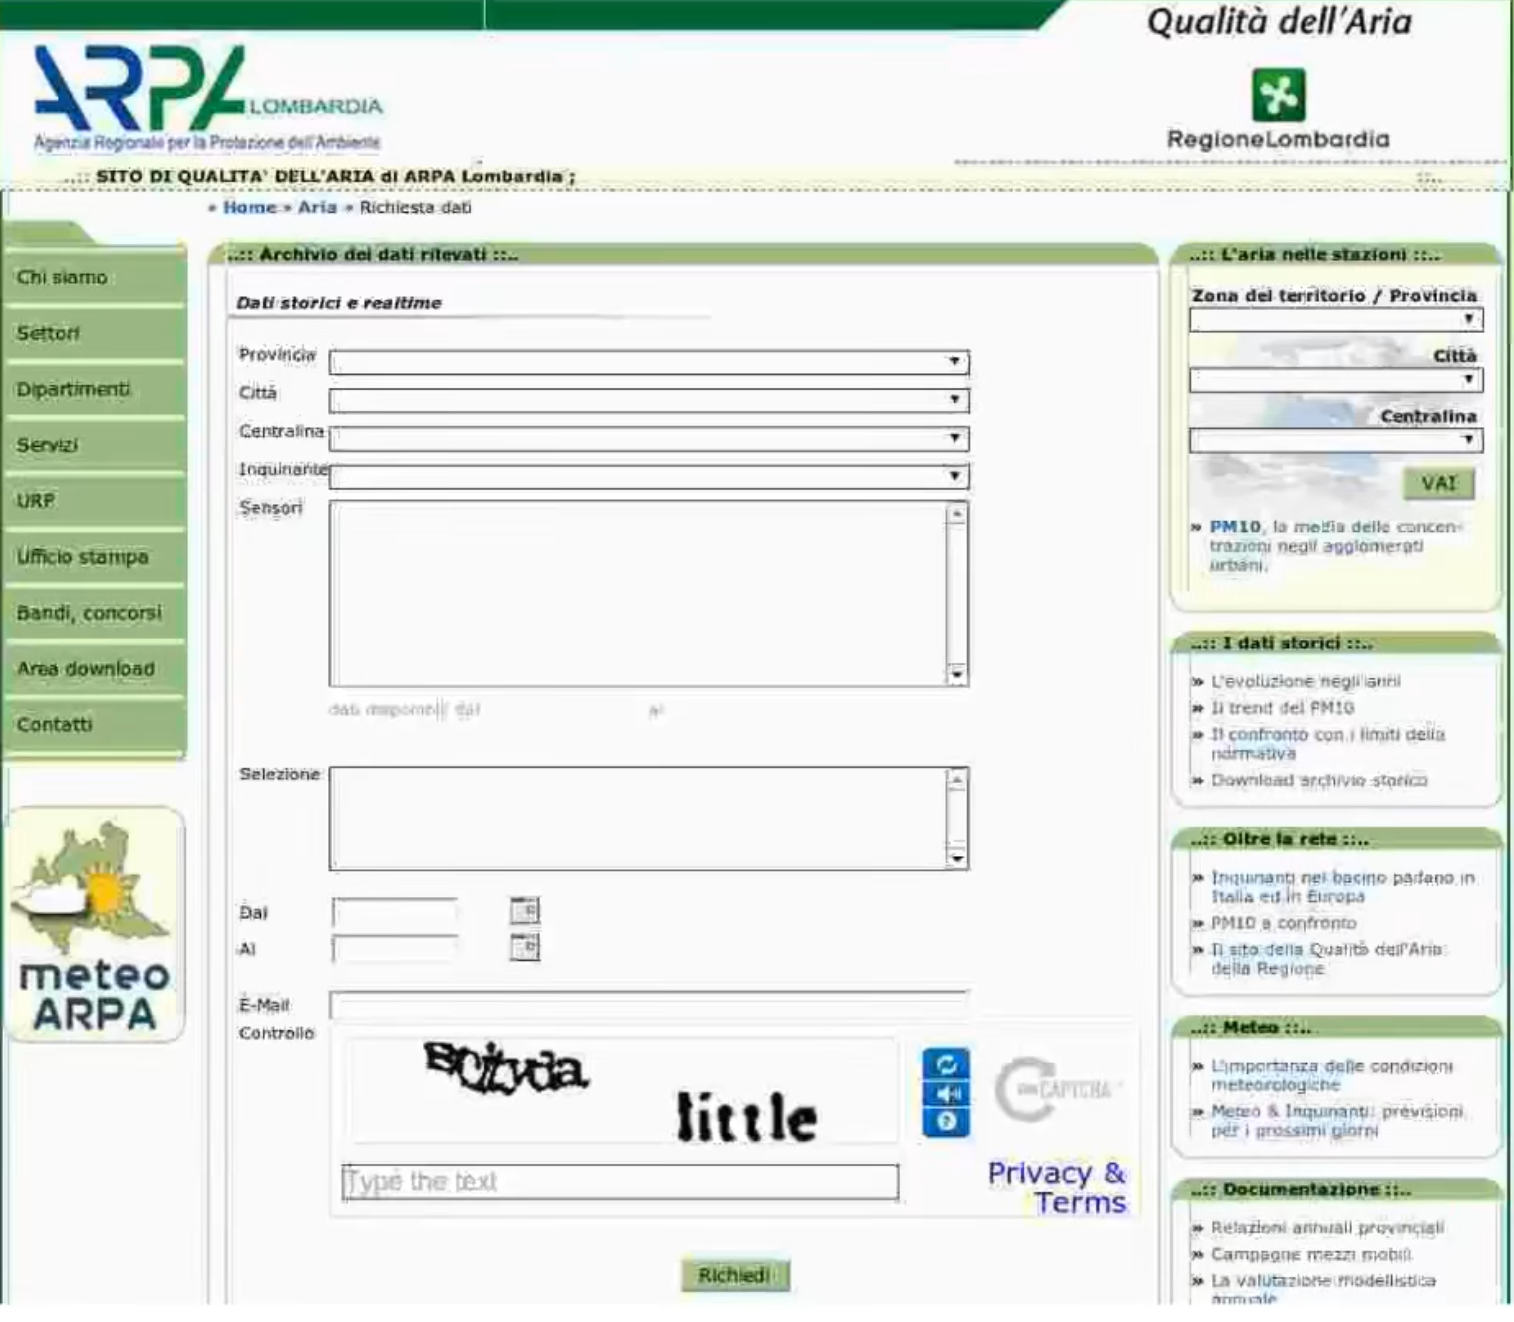
\includegraphics[width=0.7\linewidth]{img/arpa.png}\hspace*{\fill}
    \caption{Vecchio sito Arpa}
\end{figure}

La garanzia di \quotestyle{poter fare i conti in tasca alle istituzioni}, è un 
valore che molto spesso è contrapposto al diritto alla privacy, anche in 
modo completamente ingiustificato, e esisterebbero numerosi vantaggi nell'obbligare 
il rilascio di più informazioni da parte di aziende e enti. 

Questo lavoro è da intendere come una dimostrazione delle analisi realizzabili 
tramite dati pubblici, e di quanti altri studi sarebbe possibile eseguire se fossero 
disponibili le informazioni mancanti.

Tra le domande che ci si porrà, ci si chiederà se il pavè, a Milano, 
influisca sull'incidentalità, o se gli autovelox rendano più attenta 
la guida delle automobili in loro prossimità, o ancora se le linee dei trasporti pubblici 
influiscano in maniera positiva o negativa sugli incidenti.

Altre questioni interessanti potrebbero essere:\\
Quali sono le strade più pericolose in Italia?\\
Si ha più probabilità di essere coinvolti in un sinistro in città o 
su una strada extraurbana?\\
Le linee di trasporto pubblico influenzano il traffico positivamente o negativamente?\\
Il numero di passeggeri influisce sulla probabilità di essere coinvolti in un 
incidente?\\
Esistono fattori di distrazione per il conducente di un'automobile? 

%%%%%%%%%%%%%%%%%%%%%%%%%%%%%%%%%%%%%%%%%%%%%%%%%%%%%%
\chapter{Origine dei dati}

\section{Dati riguardanti incidenti}

La maggior parte dei dataset utilizzati in questo lavoro provengono 
dall'Istituto nazionale di statistica, in particolare 
dall'archivio\footnote{\url{https://www.istat.it/it/archivio/87539}}
di dati non geolocalizzati su incidenti stradali in Italia.
Questo dataset contiene un'ampia gamma di campi, tra cui ora, 
mese, giorno della settimana in cui è avvenuto l'incidente, 
ma anche informazioni sui passeggeri, la natura del sinistro e il tipo di strada. 
Particolarmente interessanti sono anche i campi riguardanti la categoria di incrocio 
a cui è avvenuto il sinistro, come rettilineo, rotonda o semaforo.

Per quanto riguarda i dati geolocalizzati, 
la fonte è invece il giornale online TheSubmarine \cite{SUBMARINE:1}
che, in un articolo riguardante l'incidentalità a Milano, 
ha ottenuto dall'ente Istat la pubblicazione di una parte degli 
incidenti avvenuti nella città nel 2016, con la relativa posizione.
Il dataset in questione è abbastanza scarno, contiene solamente 
l'incidente con la relativa posizione, indicata tramite coordinate geografiche.

Infine l'ultimo dataset è stato trovato sul sito di 
ACI\footnote{Automobile Club Italia} \cite{ACI:1}.
Questi dati, specifici a autostrade e strade provinciali, indicano anche il 
nome della via in cui è avvenuto l'incidente, oltre a informazioni come 
l'orario, il mese o il giorno della settimana.

\section{Dati riguardanti autovelox}

Una delle prime domande che ci si è posti, è stata se gli autovelox, installati 
nel tentativo di ridurre la velocità delle vetture, avessero influenza sul numero 
degli incidenti del luogo.

Un primo dataset individuato, che riguardasse delle posizioni 
degli autovelox fissi, è stata una mappa 
GoogleMyMaps\footnote{\url{https://www.google.com/maps/d/viewer?mid=1CBgMTvIDnbGo22-Y1f3rVcbeX4C0v_w1&ll=45.365557951599605\%2C10.03650113755961&z=8}} 
creata da un utente anonimo, dunque senza un modo di provare l'autenticità dei dati. 
Per evitare di fare uso di informazioni non corrette, si è preferito scartare 
questa fonte.

Il dataset utilizzato, invece, è stato ottenuto tramite OpenStreetMaps, 
realizzando una query per selezionare solo gli autovelox presenti a Milano. 
Per restringere il campo di ricerca a solo la città, si è fatto uso delle 
Overpass API\footnote{\url{https://overpass-turbo.eu/}}, 
specifiche per OpenStreetMaps, utilizzando il codice riportato nel riquadro seguente: 

\lstinputlisting{../src/codice_per_dati/overpass_query.txt}

Il dataset ricavato, purtroppo, non contiene informazioni riguardanti quando gli 
autovelox siano stati installati, fattore importante per capirne l'effetto 
sul traffico e sugli incidenti.
Tuttavia il sito web ztlmilano \cite{ZTLMILANO:1}
contiene un articolo nel quale specifica una lista di 
autovelox installati nel 2014. 
Sapendo che il dataset di OpenStreetMaps è stato aggiornato fino ad oggi, 
è possibile ricavare la posizione precisa di questi ultimi.

La lista di Ztlmilano contiene i seguenti autovelox: 

\begin{center}
    \def\arraystretch{1.5}%  
    \begin{tabular}{ |c|c| } 
    \hline
    Numero & Localizzazione dell'autovelox \\ 
    \hline
    \rowcolor{TableGray}
    1   &   Viale Monteceneri  dir. Lugano\\
    2   &   Viale Monteceneri dir. Serra\\
    \rowcolor{TableGray}
    3   &   Cavalcavia del Ghisallo\\
    4   &   Viale Serra \\
    \rowcolor{TableGray}
    5   &   Viale Serra\\
    6   &   Via Fermi\\
    \rowcolor{TableGray}
    7   &   Viale Fulvio Testi direz. perif.\\
    8   &   Viale Fulvio Testi direz. centro\\
    \rowcolor{TableGray}
    9   &   Viale Palmanova  direz. centro\\
    10  &   Viale Palmanova\\
    \rowcolor{TableGray}
    11  &   Via Ferrari direz. Ripamonti\\
    12  &   Via Ferrari\\
    \rowcolor{TableGray}
    13  &   Via Chiesa Rossa\\
    14  &   Via dei Missaglia direz. centro\\
    \rowcolor{TableGray}
    15  &   Via dei Missaglia direz. periferia\\
    16  &   Viale Famagosta\\
    \rowcolor{TableGray}
    17  &   Via Parri\\
    18  &   Via Parri\\
    \hline
    \end{tabular}
    \label{ztl-milano}
\end{center}

Il campi della tabella ripetuti sono dovuti al fatto che alcuni autovelox sono stati 
installati in entrambe le direzioni.

\section{Dati riguardanti patentati}

Un'importante necessità in un indagine di questo tipo, è avere un contesto con cui 
interpretare i risultati ottenuti. 
Non è possibile, per esempio, dire se su una certa strada si ha un numero alto di 
incidenti, senza sapere quante automobili passano in una giornata.

Si è dunque tentata una ricerca, infruttuosa, di dataset sul traffico stradale nel periodo 
dal 2010 al 2018.
Non avendo trovato alcuna informazione sull'argomento, si è tentato di realizzare 
alcune stime del numero di automobili per regione, e a Milano.

I dati sui patentati per regione, che è stato utilizzato per stimare il traffico 
regionale, proviene dal sito del Ministero delle Infrastrutture e 
Trasporti\footnote{\url{http://dati.mit.gov.it/catalog/dataset/patenti}}.
Questo dataset è diviso in vari file seconda della regione e, vista la quantità 
non necessaria di informazioni, si è preferito usare informazioni provienienti da 
un'infografica che sintetizza i dati in questione \cite{INFOGRAFICA_MIT:1}.
In particolare, da questo file pdf si è mantenuto solamente il numero di patenti per regione.

\'E anche necessario chiedersi quanto il numero dei patentati per regione sia uno stimatore 
valido per il traffico, tenendo conto del fatto che molte persone non vivono nella regione 
in cui hanno ottenuto la patente, e altre potrebbero spostarsi ogni giorno in altri 
luoghi per questioni di lavoro. 
Va dunque tenuto conto che questa stima non sarà probabilmente tra le più accurate, 
e in caso di grandi disparità tra regioni, si potrebbe dover invalidare i calcoli eseguiti.

\section{Dati riguardanti le zone di Milano}

I dati con zone geolocalizzate di Milano provengono dal geoportale del comune di 
Milano\footnote{\url{https://geoportale.comune.milano.it/}}, e contengono i poligoni che 
costituiscono i municipi della città, 
oltre a informazioni sulla superficie e il perimetro delle zone.

Questi dati sono utili a determinare, a grandi linee, quali sono le zone con più incidenti 
a Milano, tuttavia il risultato ottenuto non sarà mai preciso, 
soprattutto per l'ampiezza delle sezioni.
Un altro problema, è che le zone non contengono solamente la superficie stradale, ma anche 
abitazioni e terreni, in cui non avverranno mai incidenti. 
Ciò rende inutile la misura dell'area della zona.

\section{Dati riguardanti il meteo}

Per quanto riguarda i dati su meteo, si è tentato di utilizzare le informazioni 
provenienti dalle centraline Arpa, tuttavia, dopo veloce analisi, visibile 
in figura \ref{fig:centraline-arpa}, si è notato i dataset non 
contengono tutte le stazioni.

\begin{figure}
    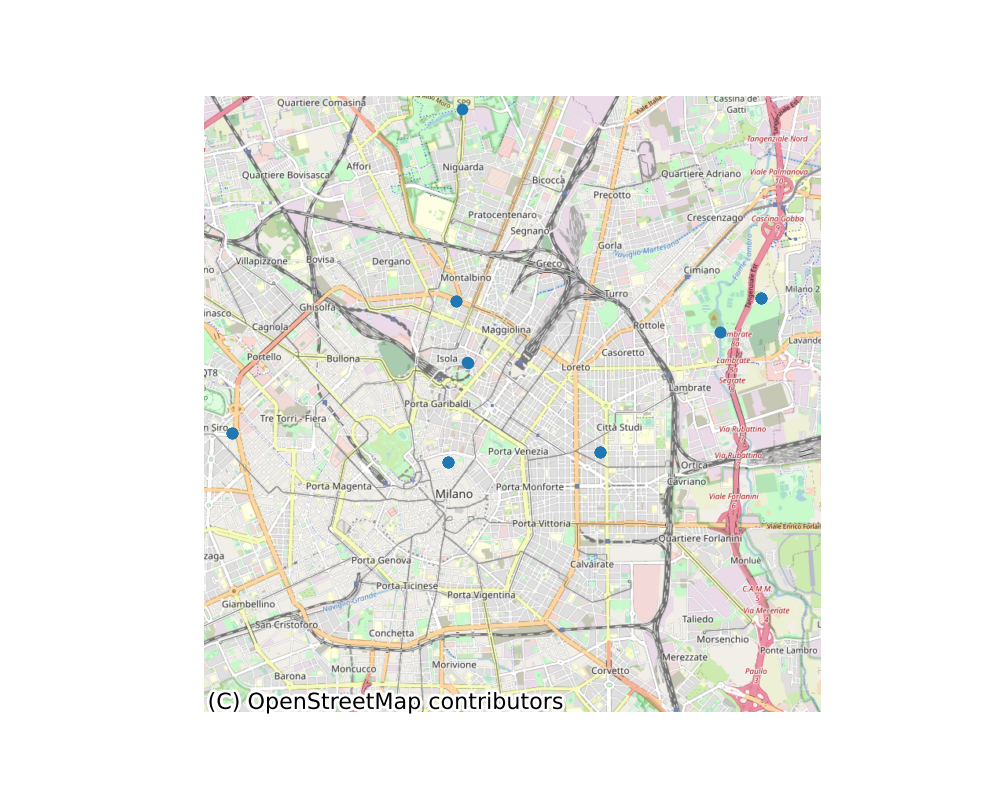
\includegraphics[width=\linewidth]{../src/meteo/centraline_arpa.png}
    \caption{Centraline Arpa a Milano}
    \label{fig:centraline-arpa}
\end{figure}

Durante un controllo della mappa \ref{fig:centraline-arpa}, ci si è accorti 
che non tutte le centraline di Milano sono contenute nel dataset.
Per esempio, utilizzando una lista di centraline meteo completa, come quella su 
Centrometeolombardo\footnote{\url{http://www.centrometeolombardo.com/content.asp?CatId=272&ContentType=Stazioni}}, 
si nota che mancano quelle di Abbiategrasso Sud e Cardorna.

Inoltre, per mancanza di dati precisi sul giorno degli incidenti, avere un'informazione così 
precisa sul meteo è superfluo.
Si è dunque optato per un dataset contenente temperature, umidità, e velocità del vento, 
trovato sul sito Zenodo\footnote{\url{https://zenodo.org/record/3992354}}.

Il dataset contiene i campi di cui si è parlato, misurati ogni ora, a partire dal 2008, 
fino al 2018.

\section{Dati riguardanti trasporti pubblici}

I dati riguardanti i trasporti pubblici trovati hanno due provenienze, i primi sono 
dati riferiti alle linee ATM, scaricati sul sito del comune di 
Milano\footnote{\url{https://dati.comune.milano.it/dataset/ds532-atm-composizione-percorsi-linee-di-superficie-urbane}}.
Dallo stesso sito proviene anche il dataset riguardante gli autobus turistici, che 
contiene in particolare le aree di sosta di questi 
ultimi\footnote{\url{https://dati.comune.milano.it/dataset/ds740_sosta_bus_gt_turistici}}.

La principale funzione di questi dataset è l'ottenere i percorsi delle linee di trasporto pubblico, 
per confrontare il numero di incidenti, tuttavia si è anche fatto uso di un dataset contenente 
solamente le linee tranviarie, trovato sul geoportale del comune di 
Milano\footnote{\url{https://geoportale.comune.milano.it/ATOM/SIT/DBT2012/DBT2012_STRATO_01_Dataset_1.xml}}.

Questo dataset è molto ampio e contiene altri livelli di informazioni, tra cui per esempio, 
le strade, le ferrovie o le piste ciclabili passanti per Milano. 

\section{Dati riguardanti autostrade e manto stradale}

Il primo dataset individuato, riguardante il manto  stradale, è stato quello di 
ANAS\footnote{\url{http://dati.mit.gov.it/catalog/dataset/grafo-stradale-anas}}, 
tuttavia questo consisteva in un file molto grande, e dalla precisione superflua per 
le mappe che si sta tentando di ottenere.

Si è dunque tentato di utilizzare il dataset presente sul geoportale del comune di 
Milano\footnote{\url{https://geoportale.comune.milano.it/}}, 
contenente anch'esso troppe strade in quanto traccia l'intero manto stradale del comune.

Come ultima risorsa, si è deciso di tracciare alcune mappe in geojson utilizzando 
Geojson.io\footnote{\url{https://geojson.io/}}, in particolare nella zona di Milano, 
per le principali autostrade, tangenziali e strade statali. 
Allo stesso modo, Geojson.io è stato utile a tracciare alcune aree in centro a Milano, 
per confrontare gli incidenti su pavè agli incidenti su asfalto.

\section{Dati riguardanti l'area C}

Il dataset riguardante gli accessi all'area C è stato trovato sul sito 
di open data del comune di 
Milano\footnote{\url{https://dati.comune.milano.it/organization/comunedimilano?q=area+c&sort=score+desc\%2C+metadata_modified+desc}}, 
dove sono disponibili varie tipologie di file distinti per esempio, per orario, 
mese o località. 
Tra questi si è utilizzata la tipologia contenente orari e data dell'accesso.

Oltre a utilizzare i dati riguardo agli accessi all'area C, si è fatto uso anche di una mappa 
raffigurante i varchi di entrata e i limiti del centro storico, 
proveniente dal sito del comune di 
Milano\footnote{\url{https://www.comune.milano.it/aree-tematiche/mobilita/area-c}}.

\section{Dati riguardanti il turismo}

I dati sul turismo in Italia, sono stati presi dall'archivio istat sul 
tema\footnote{\url{https://www.istat.it/it/archivio/16777}}.

I dati originali sono in formato xls, contenente informazioni a partire dal 1995 
fino al 2019, sia regione per regione, sia divise per nord, centro e sud.
Sono anche presenti più tabelle, ognuna rafficurante un particolare indicatore, 
come produttività del lavoro, turismo nei mesi non estivi, tasso di turisticità 
e valore aggiunto del turismo.

Per realizzare la stima, sono stati necessari i dati regione per regione, 
a partire dal 2010 fino al 2018, convertiti in formato csv, si sono scelti gli indicatori di 
turismo nei mesi non estivi, e tasso di turisticità. 

\section{Immagini del traffico}

Le immagini raffiguranti il traffico in tempo reale sono prese da Google 
Maps\footnote{\url{https://www.google.com/maps/}}, 
tuttavia questi snapshot contengono molti punti di interesse che coprono informazioni importanti, 
come i nomi delle strade.

Per rimuovere i punti di interesse, si sono utilizzate le API di google maps, 
tramite il sito Jsfiddle\footnote{\url{https://jsfiddle.net/}}.

Si sono infine realizzati degli screenshot della zona dei Navigli e dell'incrocio tra viale 
Bianca Maria e viale Ventidue Marzo.

%%%%%%%%%%%%%%%%%%%%%%%%%%%%%%%%%%%%%%%%%%%%%%%%%%%%%%
\section{Dati mancanti}

\subsection{Dati riguardanti pavè}
Non sembra che esista un dataset contenente la composizione del manto stradale di Milano.
I dati in questione sono stati cercati sui principali siti di opendata
\footnote{\url{https://dati.comune.milano.it/dataset}}
\footnote{\url{https://www.dati.lombardia.it/}}
\footnote{\url{https://www.dati.gov.it/}}
tramite parole chiave come \quotestyle{strada}, \quotestyle{manto stradale}, 
\quotestyle{pave}, \quotestyle{composizione strada}.

Una possibile risorsa trovata è una mappa utilizzata in un articolo del blog urbanfile \cite{URBANFILE:1}
Dopo una rapida consultazione tuttavia, non risulta esserci alcun dataset contenente informazioni 
riguardanti il pavè a Milano, infatti la cartina è stata realizzata tramite conoscenza personale dell'autore dell'articolo.

Il dataset che potrebbe avvicinarsi di più ad ottenere le informazioni cercate potrebbe essere 
quello riguardante i percorsi dei trasporti tranviari. Basandosi su queste informazioni, e assumendo che 
la maggior parte delle linee dei tram a Milano sono pavimentate in pavè, è possibile ottenere un dataset con taglia discreta.

\'E possibile confrontare il dataset ottenuto con la mappa di Urbanfile e, 
per quanto alcune linee coincidano, non si è trovata somiglianza sufficiente 
per giustificare la stima.

Come ultima spiaggia, si è deciso di tracciare una mappa utilizzando 
Geojson.io\footnote{\url{https://geojson.io/}}, come già fatto per le autostrade a Milano, 
basandosi sulla cartina di Urbanfile. 

\subsection{Dati riguardanti traffico stradale}
Per quanto riguarda i dati sul traffico stradale, anche in questo caso non è stato trovato un 
dataset, sia nei siti di cui si è parlato in precedenza, sia su quello di 
autostrade\footnote{\url{http://www.autostrade.it/it/home}}.

Il primo tentativo, per avere una stima del traffico è stato la realizzazione di uno script per 
fare scraping da Google Maps. Quest'ultimo infatti mostra sia il traffico in tempo reale, sia 
il traffico stimato a una determinata ora. Tuttavia, leggendo nella documentazione, si è scoperto che 
non è possibile ottenere dati sul traffico stimato, per mancanza di API. 
Per quanto fosse stato possibile realizzare comunque uno script per effettuare scraping della 
quantità di traffico nelle strade, si è optato per la ricerca di un altro dataset.

Dunque si è deciso di utilizzare i dati riguardanti gli ingressi in area C a Milano, 
trovati sul sito del comune di Milano\footnote{\url{https://dati.comune.milano.it/dataset}}, 
nonostante non permetta una stima perfetta.

Un'altro dataset utilizzato per stimare il numero di automobili, è quello contenente 
il numero di patentati per regione, trovato nel sito del Ministero dei 
Trasporti\footnote{\url{dati.mit.gov.it/catalog/dataset/patenti}}.
I dati, riguardanti i patentati fino al 2019, sono divisi in file per regione e 
contengono anche informazioni riguardanti la provincia e data di conseguimento della 
patente, oltre al tipo di ceritificato ottenuto.

\subsection{Dati su strade, incroci, semafori}

In alcuni capitoli, in particolare quelli riguardanti le tipologie di incidente e 
di incrocio, i dati che non si ha a disposizione, sono soprattutto quelli sul 
numero totale di categoria di strade.

Si è innanzi tutto tentata una ricerca, in generale, di articoli o dataset online, con 
parole chiave come \quotestyle{numero di semafori Milano} o \quotestyle{strade incroci semafori}.
Non trovando alcun riscontro, si è ricercato l'argomento nei principali siti contenenti 
dataset, elencati in precedenza. 

Le informazioni più simili a ciò che si stava cercando, sono state trovate sul geoportale 
del comune di Milano, nel dataset del manto stradale.
Questo dataset contiene vari layer di informazioni, tra cui Area di circolazione veicolare, 
Area di circolazione pedonale e Area di circolazione ciclabile, tuttavia, in nessuno 
di questi livelli, si sono trovate informazioni utili a dividere, per esempio, 
intersezioni segnalate da incroci con semaforo. 

Inoltre, per maggior parte dei livelli, non si sono trovate informazioni sul significato 
delle colonne presenti nei dataset come, per esempio, \columnstyle{GZ\_STR\_TY} o 
\columnstyle{GZ\_STR\_TYF}. 
Le ricerche per un file contenente informazioni sui metadati sono state eseguite sia 
sul sito del comune di Milano, sia in generale, tramite motore di ricerca, con parole chiave 
come \quotestyle{ID\_ZRIL milano} o \quotestyle{ID\_ZRIL metadati}. 
Nel caso di quest'ultimo, tuttavia, è risultato che fosse un identificatore univoco del 
territorio, informazione ricavata tracciando una parte dei valori della colonna.

%%%%%%%%%%%%%%%%%%%%%%%%%%%%%%%%%%%%%%%%%%%%%%%%%%%%%%
\chapter{Dati Geolocalizzati}

\section{Incidenti}

I dati riguardanti incidenti geolocalizzati, sono disponibili in un dataset contenente una 
lista di punti indicanti latitudine e longitudine dell'incidente. 
Ciò che delude, è che non è presente nessuna informazione aggiuntiva, se non la posizione 
dell'incidente.

Controllando i dati trovati, in particolare come questi siano posizionati, 
si nota dalla mappa destra nella figura \ref{fig:heatmap-municipi} che gli incidenti a Milano 
sono per buona parte uniformemente distributi per tutta la città, 
con più alte concentrazioni in alcuni punti di interesse, come Piazzale Loreto, Zona Navigli 
e Monumentale, e Corso Ventidue Marzo.

Sarebbe interessante sapere se esistono zone con maggiore concentrazione di incidenti rispetto 
alla media, e ottenere un indice numerico della pericolosità di una determinata zona.\\

Nella mappa sinistra della figura \ref{fig:heatmap-municipi}, si è divisa la città di Milano 
in base al municipio, ed è possibile osservare che nel centro si hanno la maggior parte degli 
incidenti.

\begin{figure}
    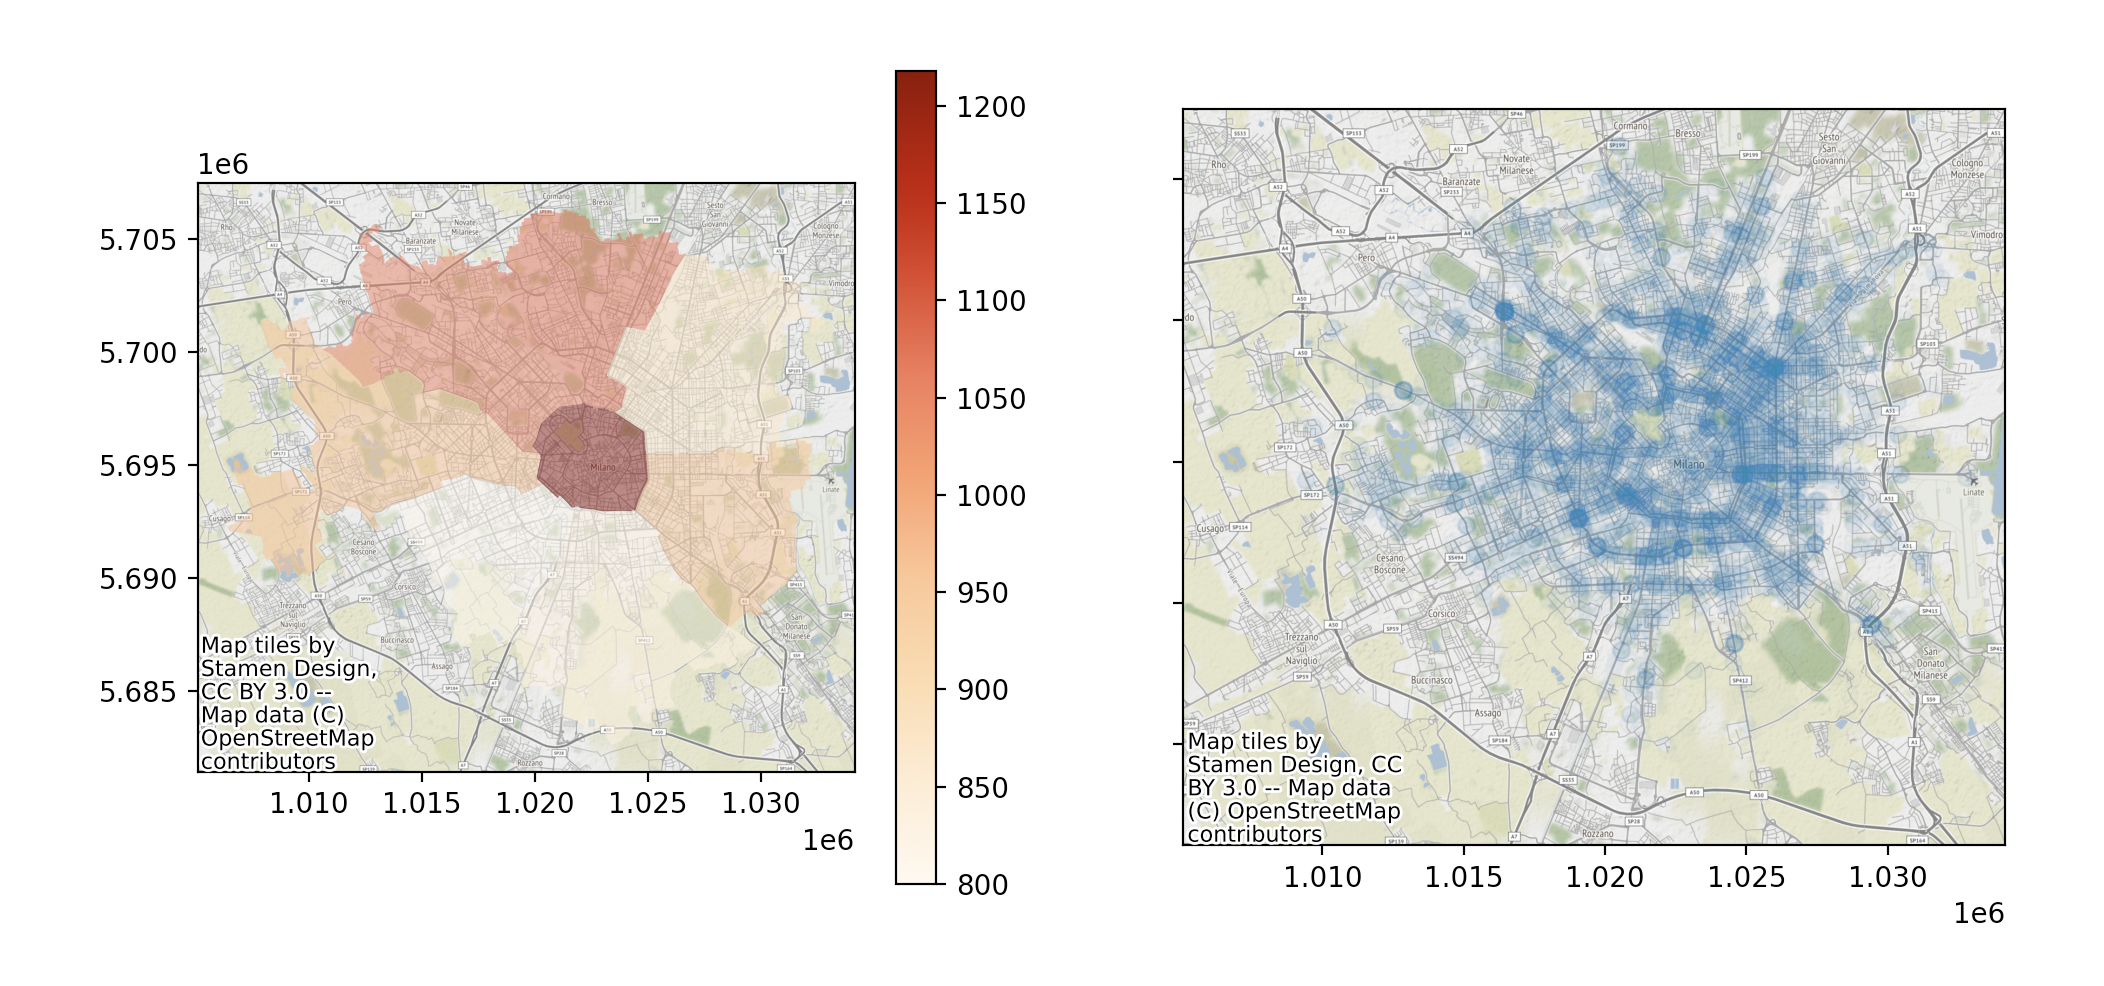
\includegraphics[width=\linewidth]{../src/municipi_milano/incidenti_municipio.png}
    \caption{Incidenti a Milano per municipio}
    \label{fig:heatmap-municipi}
\end{figure}

Non tutte le zone hanno la stessa superficie, avendo a disposizione l'area dei vari municipi, 
è possibile calcolare la media di incidenti al chilometro quadrato per zona.
I risultati sono riportati nella tabella sottostante.

\begin{lstlisting}    
    inc = gp.GeoSeries(df).sort_index()

    area = pd.Series(data['AREA'], index=data['MUNICIPIO'])
    incidenti = pd.Series(inc, index=inc.index)

    # trasformazione in chilometri quadri
    incidenti_per_zona = (incidenti / area) * 1000000 
\end{lstlisting}

\begin{center}
    \def\arraystretch{1.5}%  
    \begin{tabular}{ |c|c| } 
    \hline
    Numero della zona & Nome della zona \\ 
    \hline
    \rowcolor{TableGray}
    1   &   Centro Storico\\
    2   &   Greco, Padova\\
    \rowcolor{TableGray}
    3   &   Venezia, Città Studi\\
    4   &   Vittoria, Vigentina \\
    \rowcolor{TableGray}
    5   &   Ticinese, Gratosoglio\\
    6   &   Inganni, Barona\\
    \rowcolor{TableGray}
    7   &   Baggio, Forze Armate\\
    8   &   Gallaratese, Sempione\\
    \rowcolor{TableGray}
    9   &   Niguarda, Dergano\\
    \hline
    \end{tabular}
\end{center}

\begin{figure}
    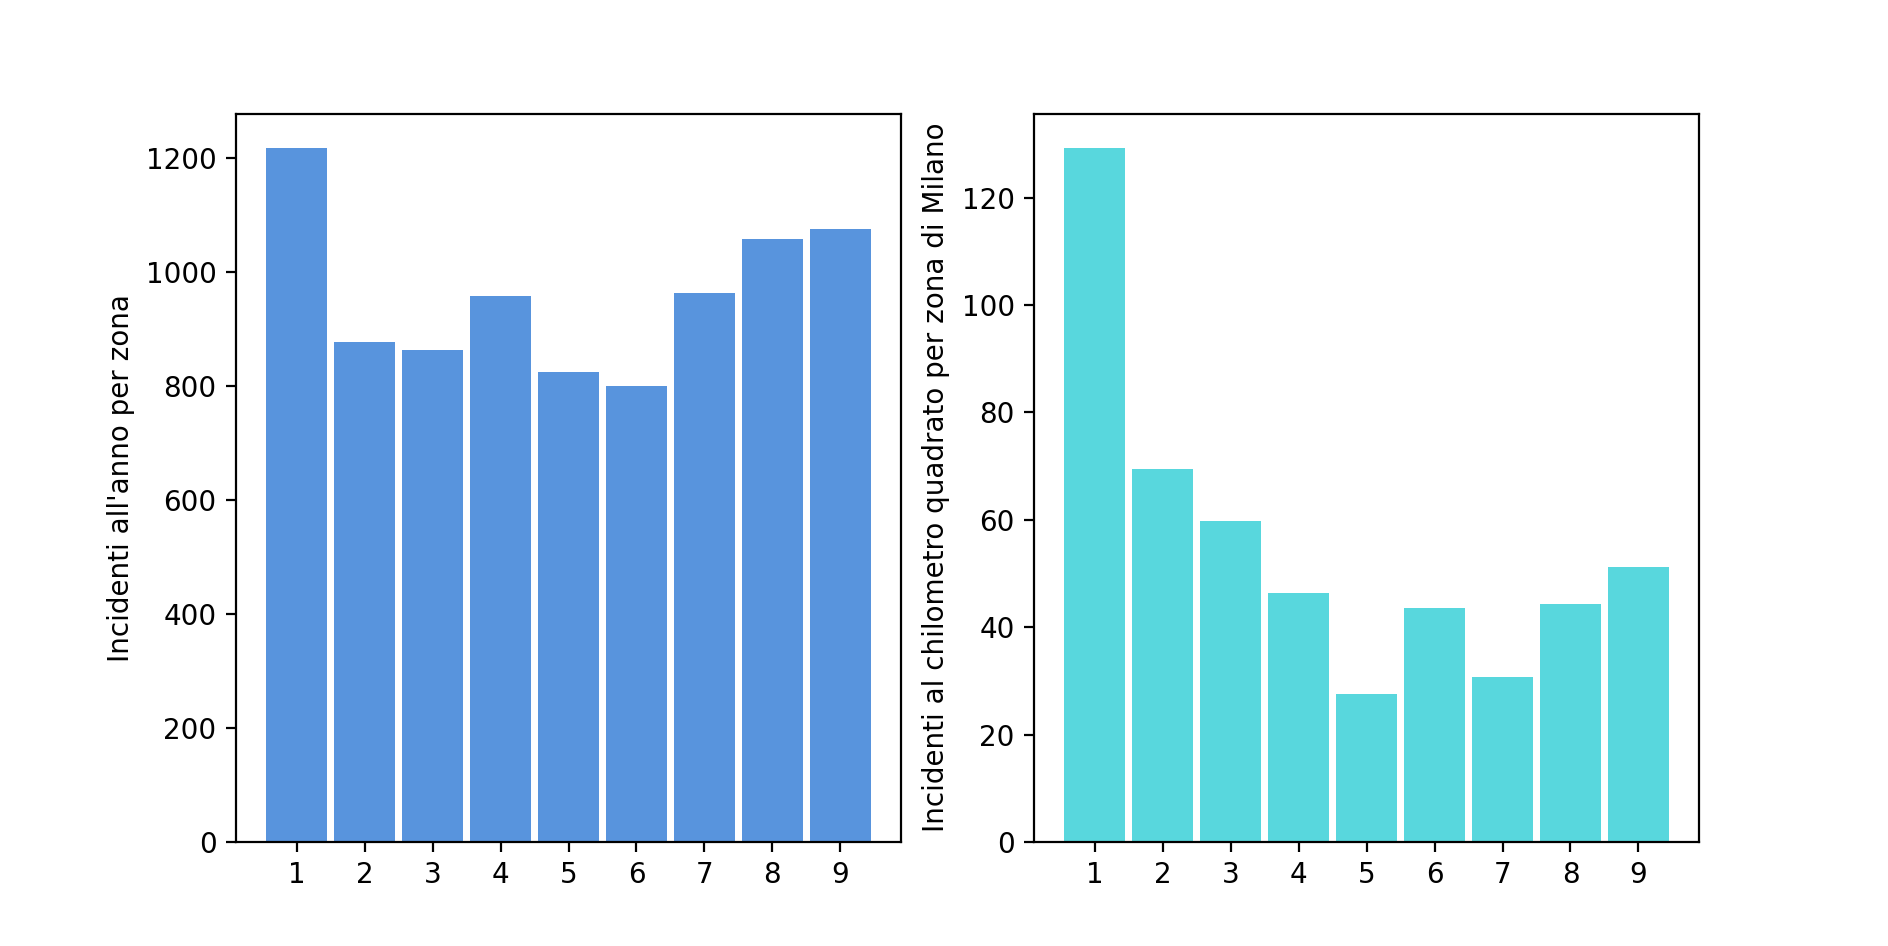
\includegraphics[width=\linewidth]{../src/municipi_milano/incidenti_superf.png}
    \caption{Incidenti a Milano per zona e in base alla superficie della zona}
    \label{fig:incidenti-chilometro}
\end{figure}

Nella figura \ref{fig:incidenti-chilometro} spicca, sia nel grafo di sinistra che in quello di destra, 
la zona 1, cioè quella del centro storico, vista la superficie minore rispetto agli altri municipi.

Una volta creata la tendenza generale del municipio, è possibile confrontare i risultati 
ottenuti con il numero di incidenti in zone più ristrette, per esempio attorno a piazzale Loreto.

\begin{figure}
    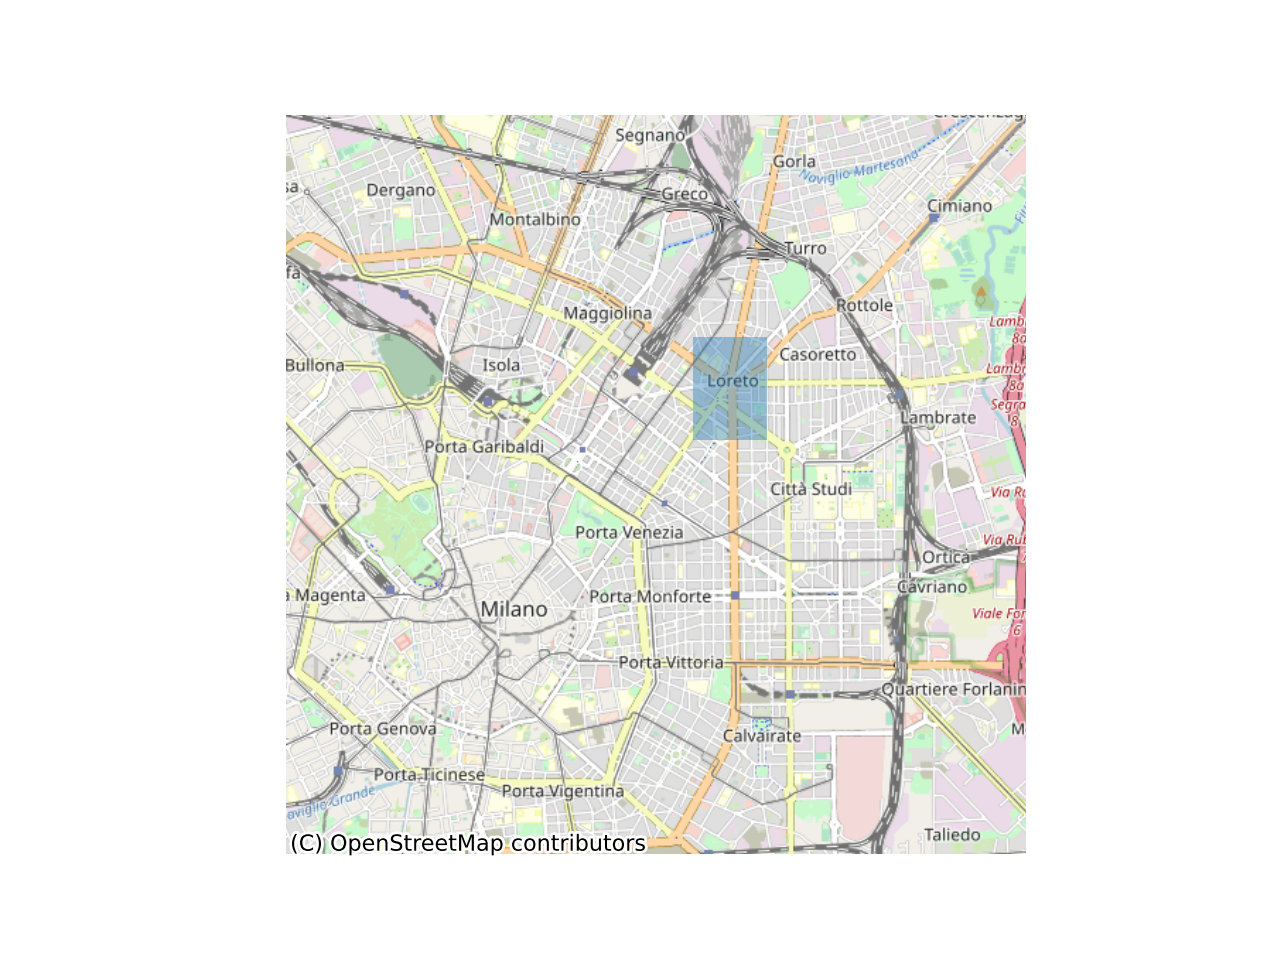
\includegraphics[width=\linewidth]{../src/municipi_milano/zona_loreto.png}
    \caption{Zona presa in considerazione per piazzale Loreto}
    \label{fig:zona-loreto}
\end{figure}

\begin{lstlisting}
    loreto = geometry.Polygon([p1, p2, p4, p3])

    loreto_incidenti = 0
    for point in incidenti['geometry']: 
        point = geometry.Point(point)

        if loreto.contains(point): 
            loreto_incidenti += 1

    area_loreto = loreto.area * data['AREA'].iloc[0] / geometry.Polygon(data['geometry'].iloc[0]).area
    area_loreto_inc = loreto_incidenti * 1000000 / area_loreto
\end{lstlisting}

Il numero di incidenti per chilometro che risultano, nell'area considerata in figura 
\ref{fig:zona-loreto}, sono 231.06, considerando che il massimo ottenuto per zona, 
il centro storico, arriva attorno a 120 incidenti per chilometro quadrato, è possibile affermare 
che piazzale loreto sia una zona ad alta incidentalità.

Una domanda che sorge spontanea è il perchè in centro storico risulti tra le aree con maggiore 
incidentalità, il volume di incidenti non dovrebbe essere abbassato della presenza dell'area C?

\begin{figure}
    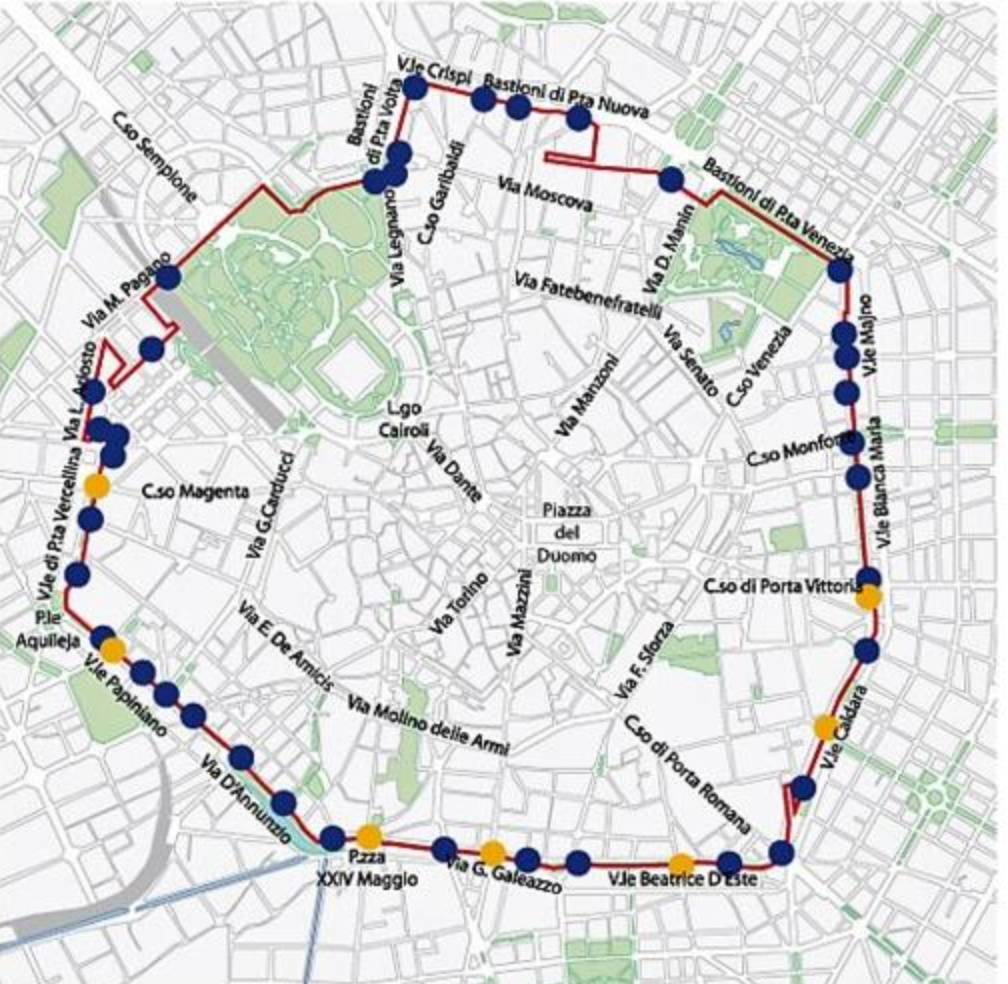
\includegraphics[width=0.48\linewidth]{../dataset/area_c/perimetro_area_c.png}
    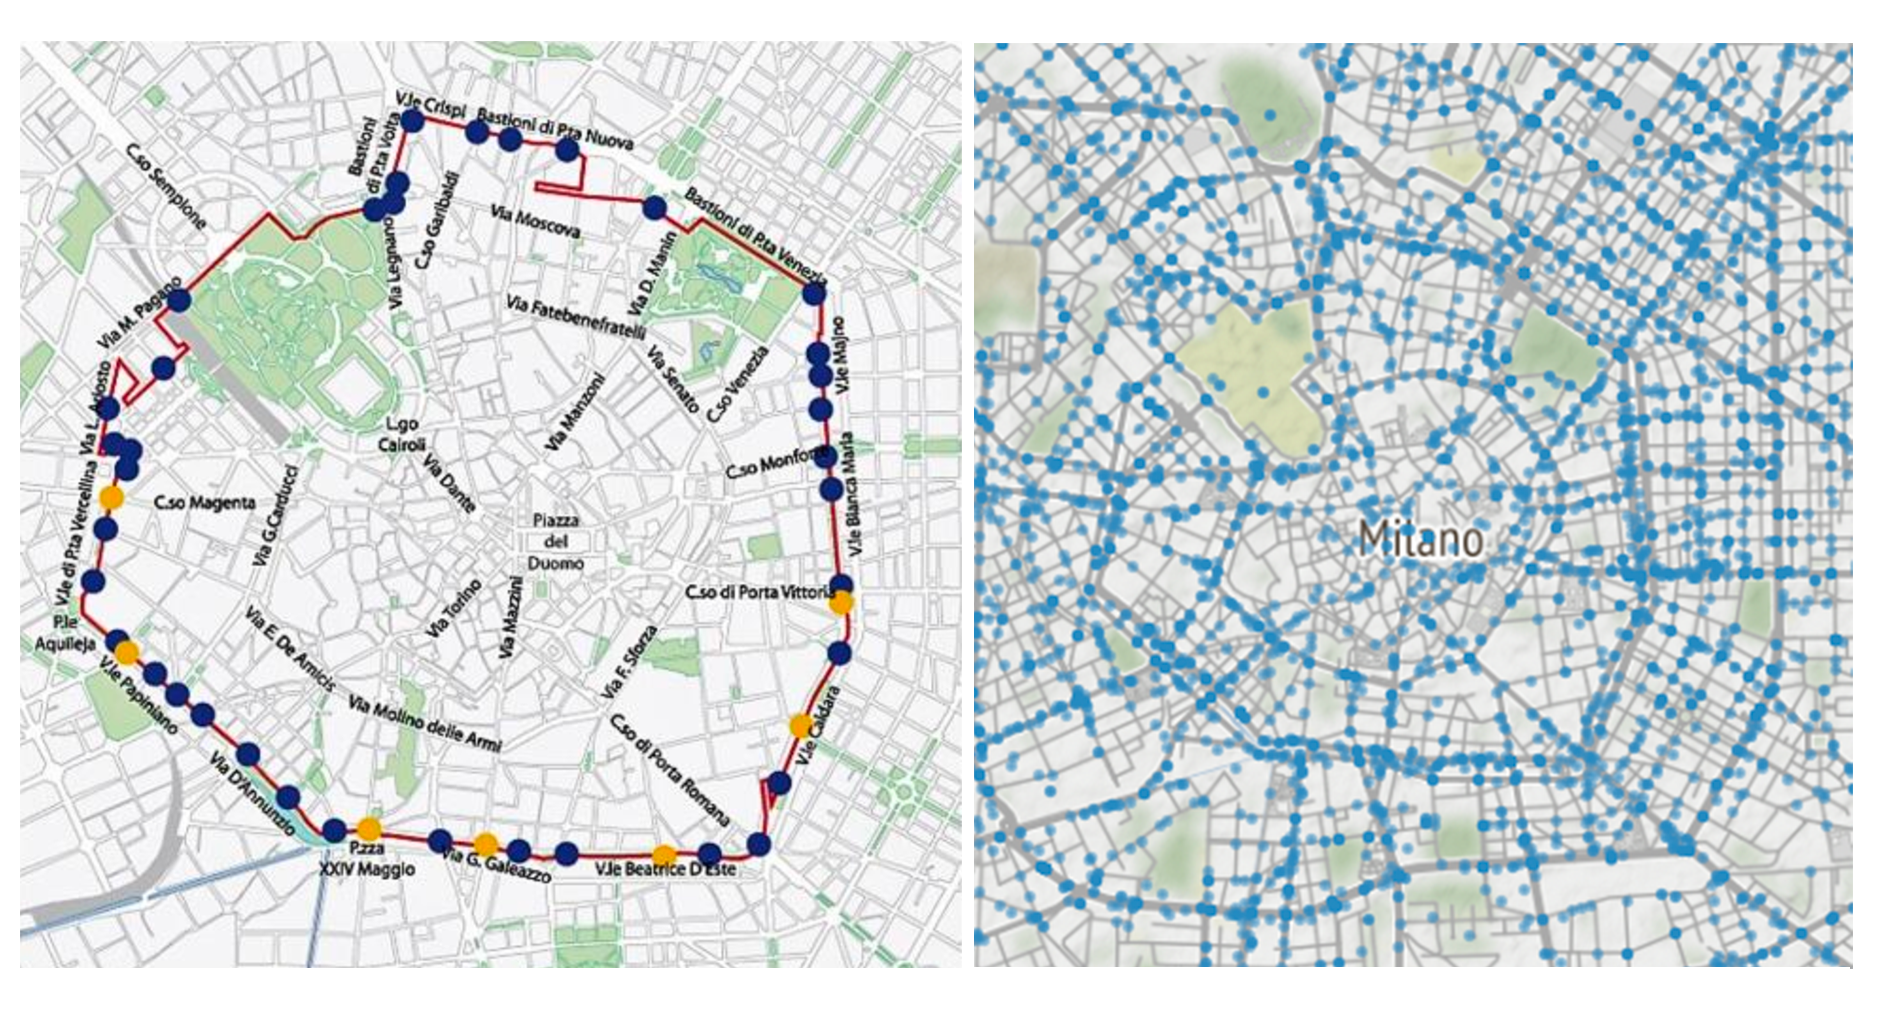
\includegraphics[width=0.52\linewidth]{../src/area_c/area_c_incidenti.png}
    \caption{Perimetro dell'area C e incidenti nella stessa zona}
    \label{fig:perimetro-area-c}
\end{figure}

Dopo più attenta osservazione del perimetro dell'area C, visibile in figura \ref{fig:perimetro-area-c}, 
si osserva che la maggior parte degli incidenti avvengono sulla circonvallazione interna, 
situata fuori dall'area C, che è compresa nell'centro storico di Milano.

Prendendo in considerazione solamente l'area C, il numero di incidenti scende a $46.83$ 
per chilometro quadrato, dunque è possibile concludere che la riduzione del traffico nel 
centro di Milano ha impatto consistente sull'incidentalità.

\begin{lstlisting}
    area_c = geometry.Polygon(gp.read_file("dataset/area_c/area_c.geojson").to_crs(epsg=3857)['geometry'].iloc[0])

    inc = 0
    for point in incidenti['geometry']: 
        if area_c.contains(geometry.Point(point)): 
            inc += 1
\end{lstlisting}

%\clearpage
\section{Incidenti e Linee dei Trasporti Pubblici}

Il dataset dei tragitti dei trasporti pubblici copre molta più superficie rispetto a 
quello degli incidenti, dopo aver eliminato alcune linee di autobus che risultavano 
troppo in periferia, si ottiene la mappa sinistra nella figura \ref{fig:geo-trasporti}: 

\begin{figure}
    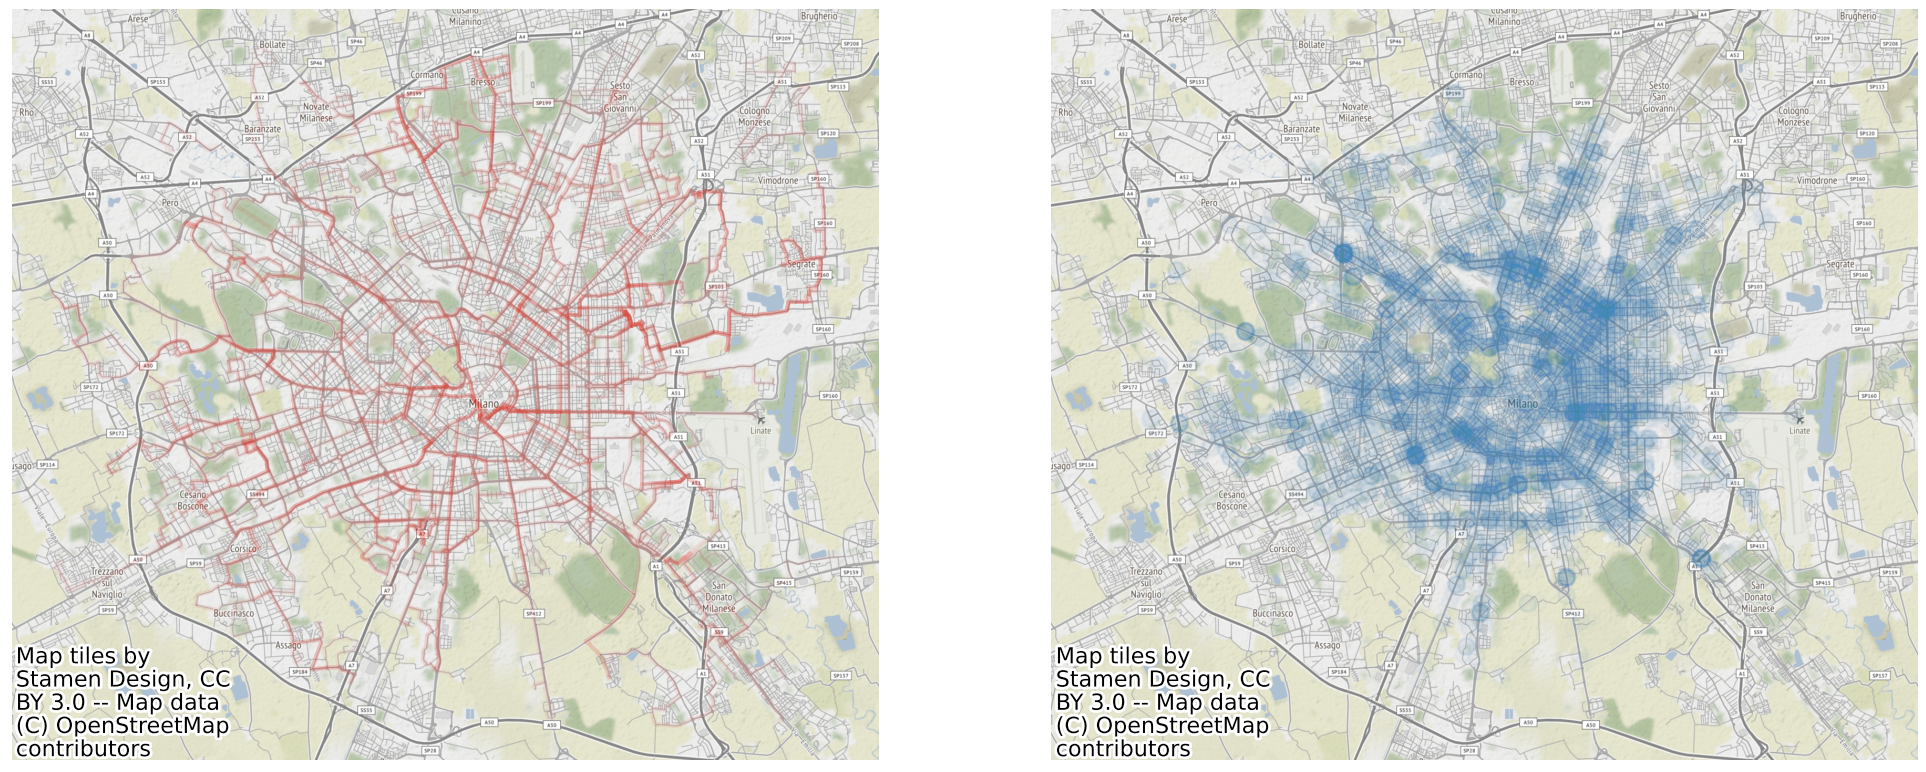
\includegraphics[width=\linewidth]{../src/atm/linee_atm.png}
    \caption{Linee Autobus e Tram a Milano}
    \label{fig:geo-trasporti}
\end{figure}

Affiancando le posizioni degli incidenti ai tragitti dei trasporti pubblici, 
non è possibile notare un collegamento preciso tra i due dataset. Sono presenti tuttavia alcune 
corrispondenze come, per esempio, la zona dei navigli e quella circostante a 
corso Ventidue Marzo. 
Sono anche visibili alcune strade con alta incidentalità, parallele a linee di autobus. 
Un esempio è quello di zona Navigli, in figura \ref{fig:navigli}, dove le vie interessate sono:
Viale Gian Galeazzo e Viale Beatrice D'Este, parallele a Viale Col di Lana e Viale Bligny.
Lo stesso fenomeno è osservabile su Viale Gabriele D'Annunzio e Viale Gorizia e Coni Zugna, 
e in un'altra zona, vicino a corso Ventidue Marzo.

\begin{figure}
    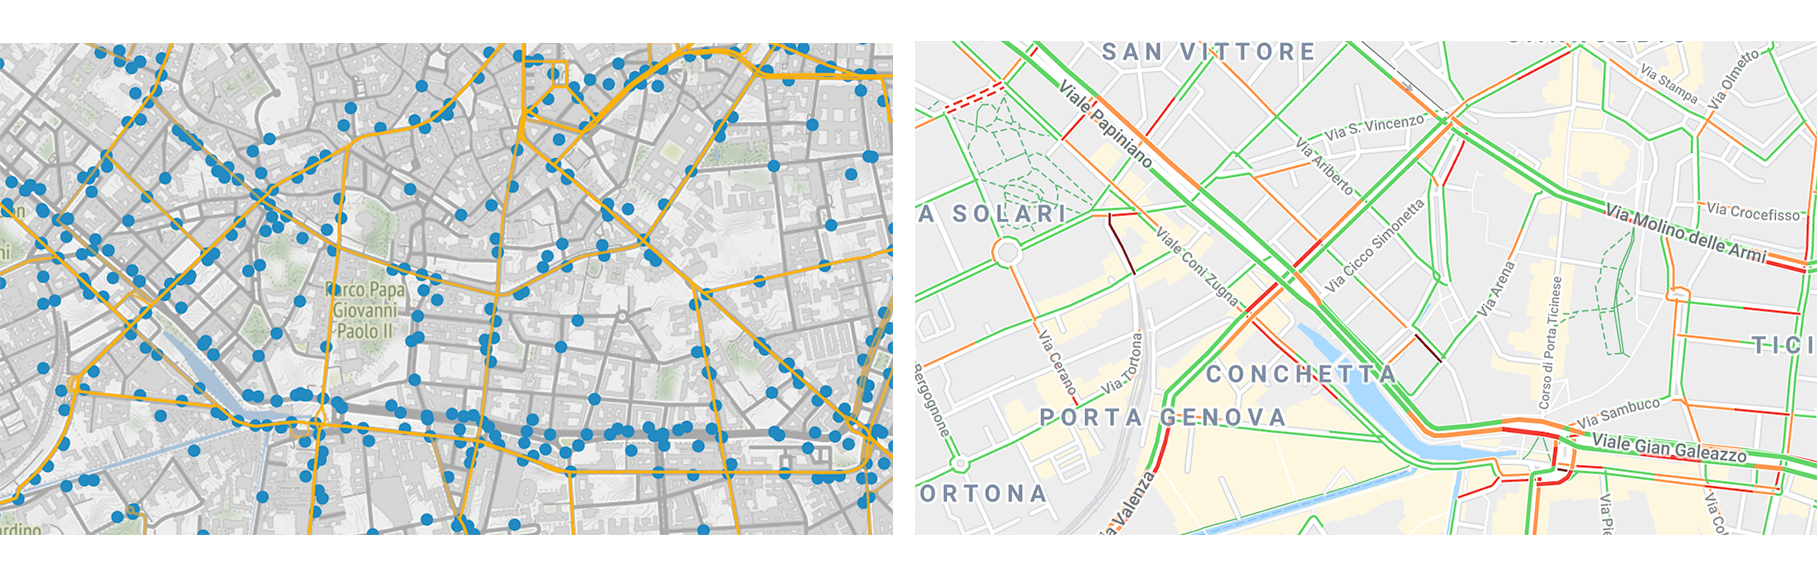
\includegraphics[width=0.51\linewidth]{../src/atm/navigli.png}
    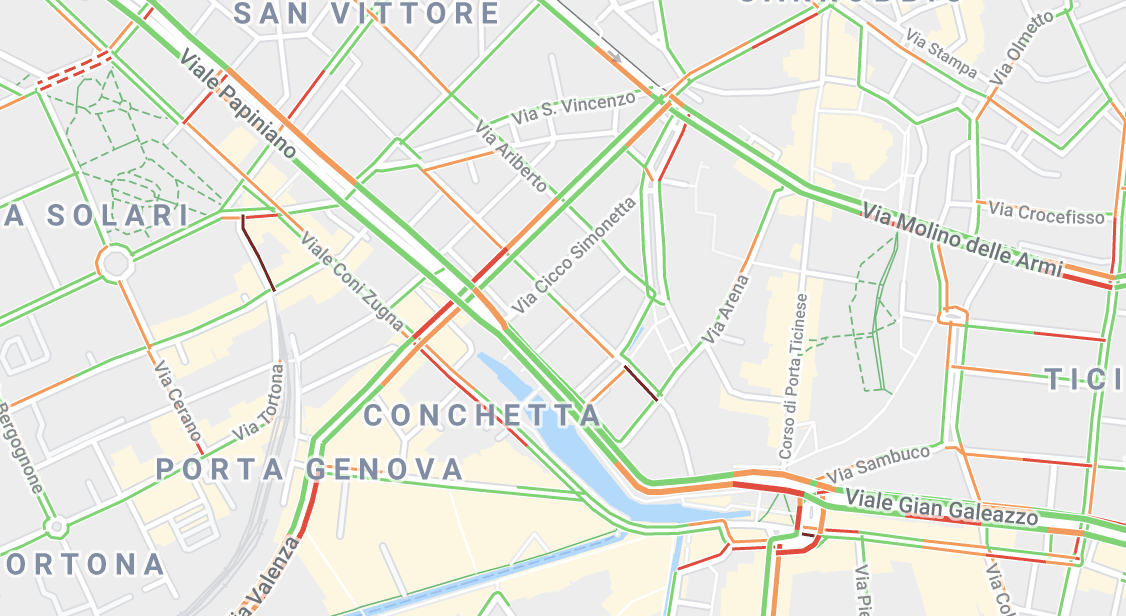
\includegraphics[width=0.49\linewidth]{img/navigli.png}
    \caption{Linee dei trasporti pubblici e condizioni di traffico nella zona Navigli}
    \label{fig:navigli}
\end{figure}

Anche vicino a corso Ventidue Marzo, nella mappa \ref{fig:22-marzo} si può 
notare lo stesso fenomeno, tra Viale Bianca Maria e Viale Premuda.

\begin{figure}
    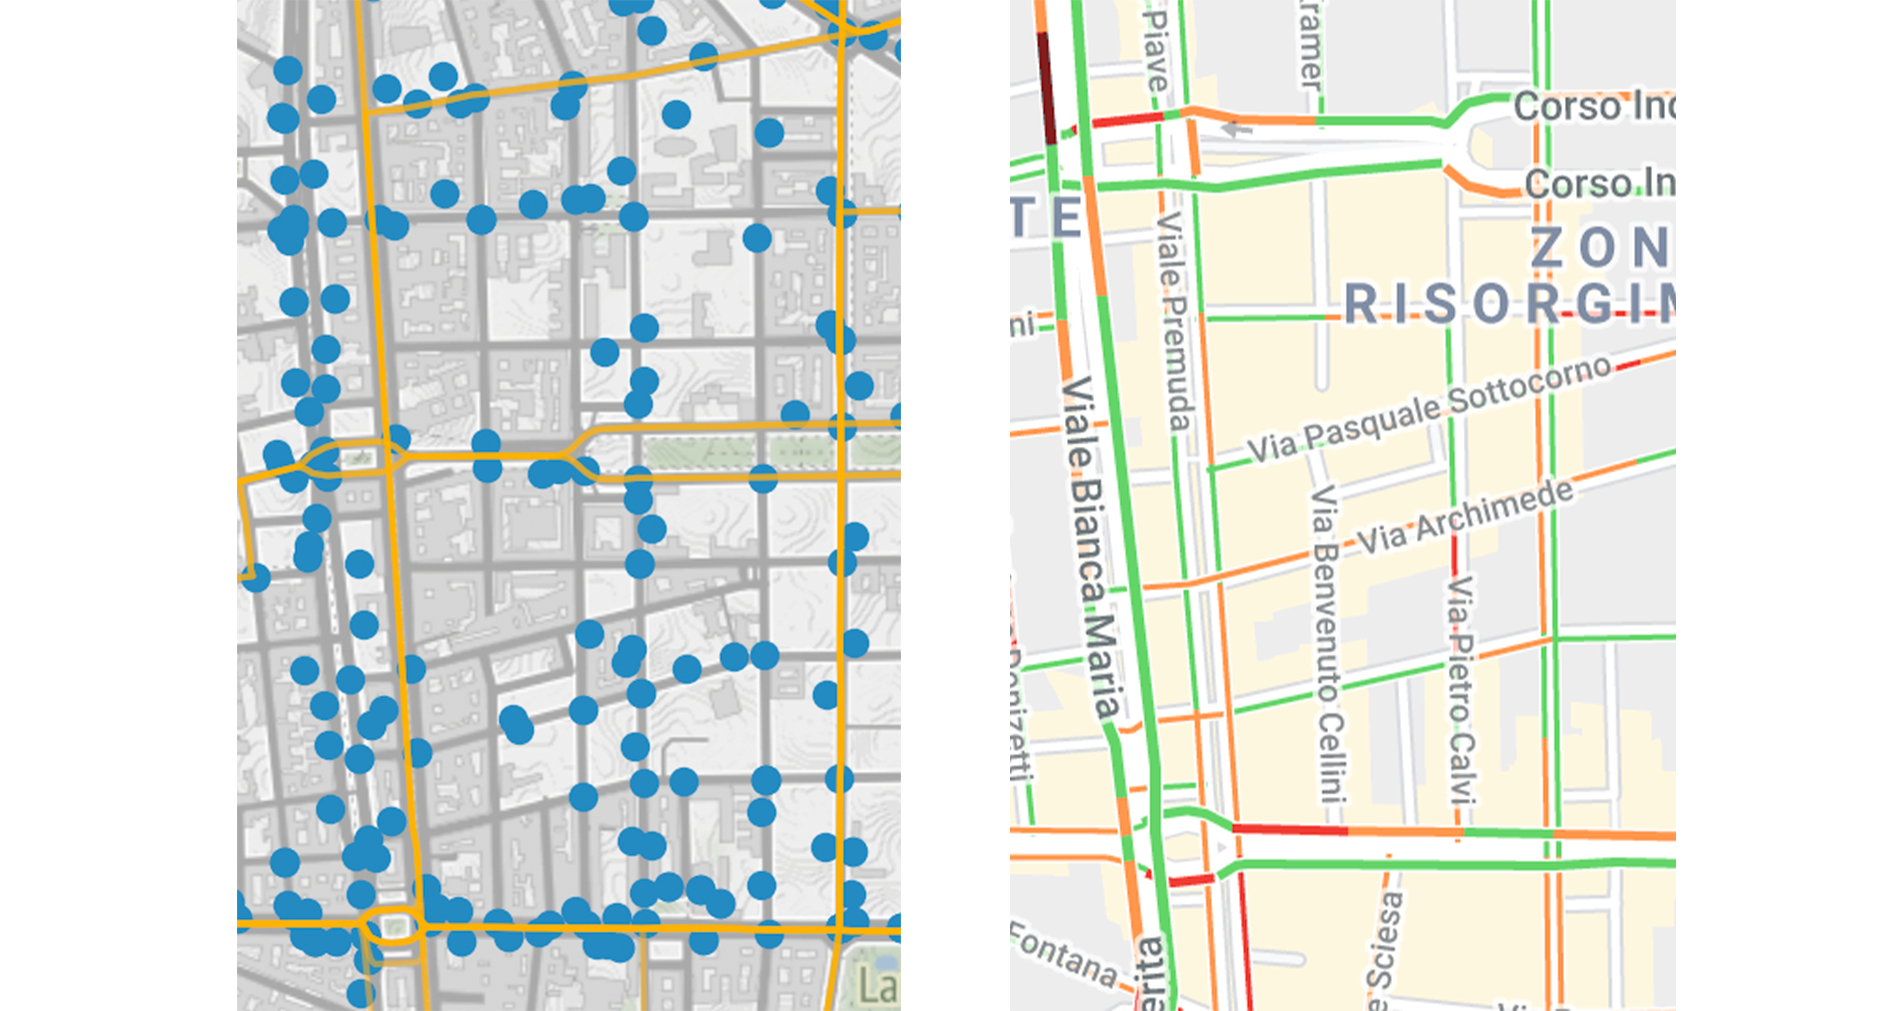
\includegraphics[width=0.25\linewidth]{../src/atm/22_marzo.png}
    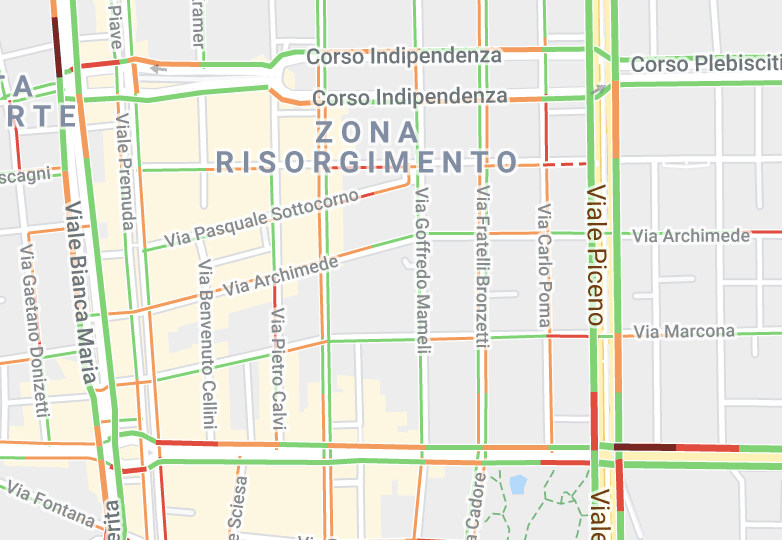
\includegraphics[width=0.55\linewidth]{img/22_marzo.png}
    \caption{Linee dei trasporti pubblici e condizioni traffico vicino a Corso Ventidue Marzo}
    \label{fig:22-marzo}
\end{figure}

Le immagini del contenenti indicazioni sul traffico sono state realizzate tramite le API di 
Google Maps, tuttavia non offrono una stima ideale, poiche indicano il traffico in tempo reale e 
il Covid-19 ha ridotto notevolmente il volume di automobili.

Per confutare l'ipotesi iniziale, si sono utilizzati i dati ricavati in precedenza, 
degli incindenti per chilometro per municipio Milano. 
Nella zona dei navigli, si è poi presa in considerazione la sezione \ref{fig:zona-navigli-rect}, 
perchè sono presenti molti incidenti in viale Papiniano e viale Beatrice d'Este, 
e un numero minore nella via parallela sottostante, in cui è anche presente 
una linea di trasporti pubblici.

\begin{figure}
    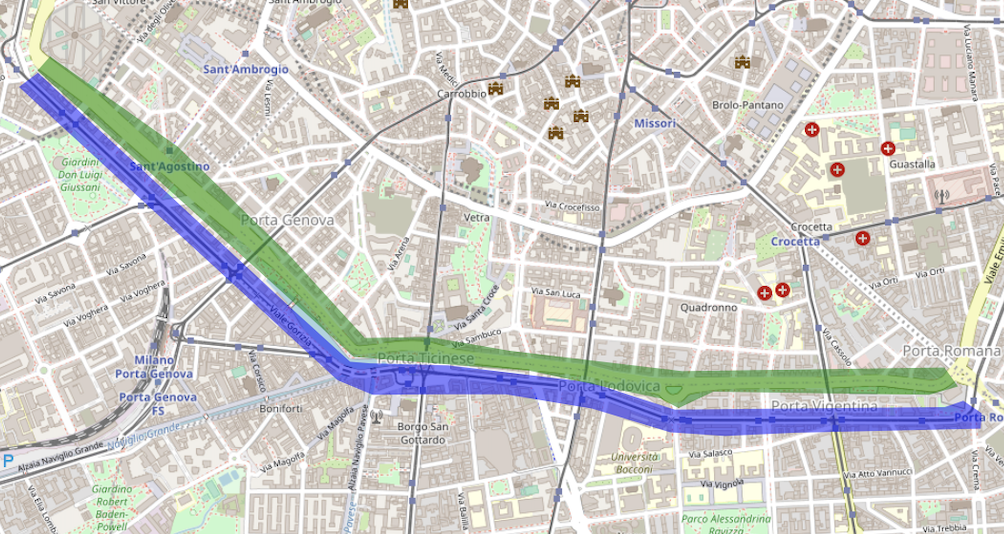
\includegraphics[width=\linewidth]{../src/atm/zona_navigli_rect.png}
    \caption{Sezioni di Milano prese in considerazione per contare gli incidenti ai navigli}
    \label{fig:zona-navigli-rect}
\end{figure}

\begin{lstlisting}
    data = gp.read_file("dataset/zone_milano/zone.geojson").to_crs(epsg=3857)
    autobus = data[data['name'] == "Navigli Autobus"]
    street = data[data['name'] == "Navigli Incidenti"]

    autobus_rect = geometry.Polygon(autobus['geometry'].iloc[0])
    street_rect = geometry.Polygon(street['geometry'].iloc[0])

    inc_a = 0
    inc_s = 0
    for point in incidenti['geometry']: 
        point = geometry.Point(point)

        if autobus_rect.contains(point): 
            inc_a += 1
        
        if street_rect.contains(point): 
            inc_s += 1
\end{lstlisting}

Il risultato, conferma che avvengono $167.09$ incidenti per chilometro 
nel viale in cui sono presenti trasporti pubblici, che per quanto non sia nella media per la zona 
di appartenenza, è giustificabile in quanto si è presa in considerazione solo la strada.
Nell'altra zona, invece, dove non passa alcuna linea di trasporti pubblici, 
gli incidenti sono $289.32$. 

Non è detto che il maggior numero di incidenti sia causato dalla linea degli autobus, 
in particolare, va tenuta in considerazione la topologia delle due vie parallele.
La differenza principale tra viale Bligny e viale Beatrice d'Este è che, il primo è una via a due 
corsie per senso di marcia, mentre il secondo è un viale a due 
carreggiate\footnote{Carreggiata: la parte della strada destinata allo scorrimento dei veicoli, 
delimitata da una striscia continua o da un paracarro} 
con sensi di marcia separati. 
Dunque è ovvio che la maggior parte dei conducenti preferiscono un viale ad alta velocità rispetto a 
una via dove è possibile rimanere incolonnati per la presenza di una sola corsia, e dove si è 
rallentati dalla presenza di autobus o tram.

Lo stesso procedimento è stato realizzato per corso Ventidue Marzo, le zone utilizzate sono 
raffigurate nel'immagine \ref{fig:zona-22marzo-rect}. 

\begin{figure}
    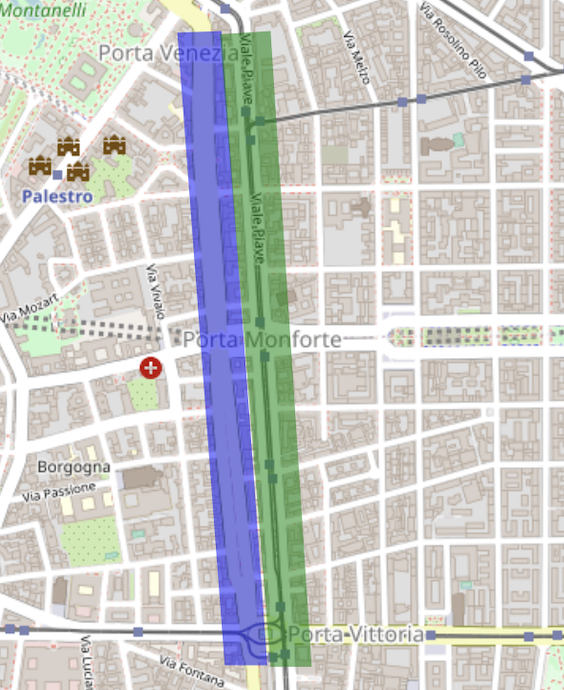
\includegraphics[width=\linewidth]{../src/atm/zona_22marzo_rect.png}
    \caption{Sezioni di Milano prese in considerazione per contare gli incidenti intorno a corso Ventidue Marzo}
    \label{fig:zona-22marzo-rect}
\end{figure}

In questo caso, per viale Bianca Maria, dove non è presente una linea di trasporti pubblici, 
il numero di incidenti è $254.31$, mentre per viale Premuda per cui passa una linea tranviaria, 
il numero scende a $93.96$.

Anche per questa zona, le due vie prese in considerazione sono molto diverse.
Viale Premuda è una via a due carreggiate separate, ognuna con una corsia e un solo senso 
di marcia, dove sono parcheggiate automobili su entambi i lati, e la velocità dei 
veicoli non deve essere particolarmente elevata.
D'altra parte viale Bianca Maria, pur avendo carreggiate separate, queste hanno due, 
e in alcuni punti tre, corsie ciascuna. 
Con l'aumentare dello spazio, inevitabilmente la velocità delle automobili aumenta, 
e con esso il rischio di incidenti.

Va sottolineato che le strade prese in considerazione hanno differenze sostanziali, e che 
difficilmente una persona alla guida, scegliendo quale strada predendere, tiene in 
considerazione i mezzi pubblici. 
I fattori che influenzano maggiormente la scelta devono essere, in primo luogo, 
il traffico, in quanto il conducente preferirà sempre dettare la propria velocità, e non 
essere rallentato o avere automobili che gli mettono fretta da dietro, 
e di conseguenza, in secondo luogo, le esperienze personali, come per esempio: 
\quotestyle{settimana scorsa sono rimasto bloccato nel traffico per un'ora su quella 
strada}.

%\clearpage
\subsection{Il pavè a Milano influisce in qualche modo sull'incidentalità?}

Spesso le linee di tram coincidono con strade in pavè, è vero per Milano? 
Tramite la mappa \ref{fig:tram-pave-milano} è possibile confrontarle: 

\begin{figure}
    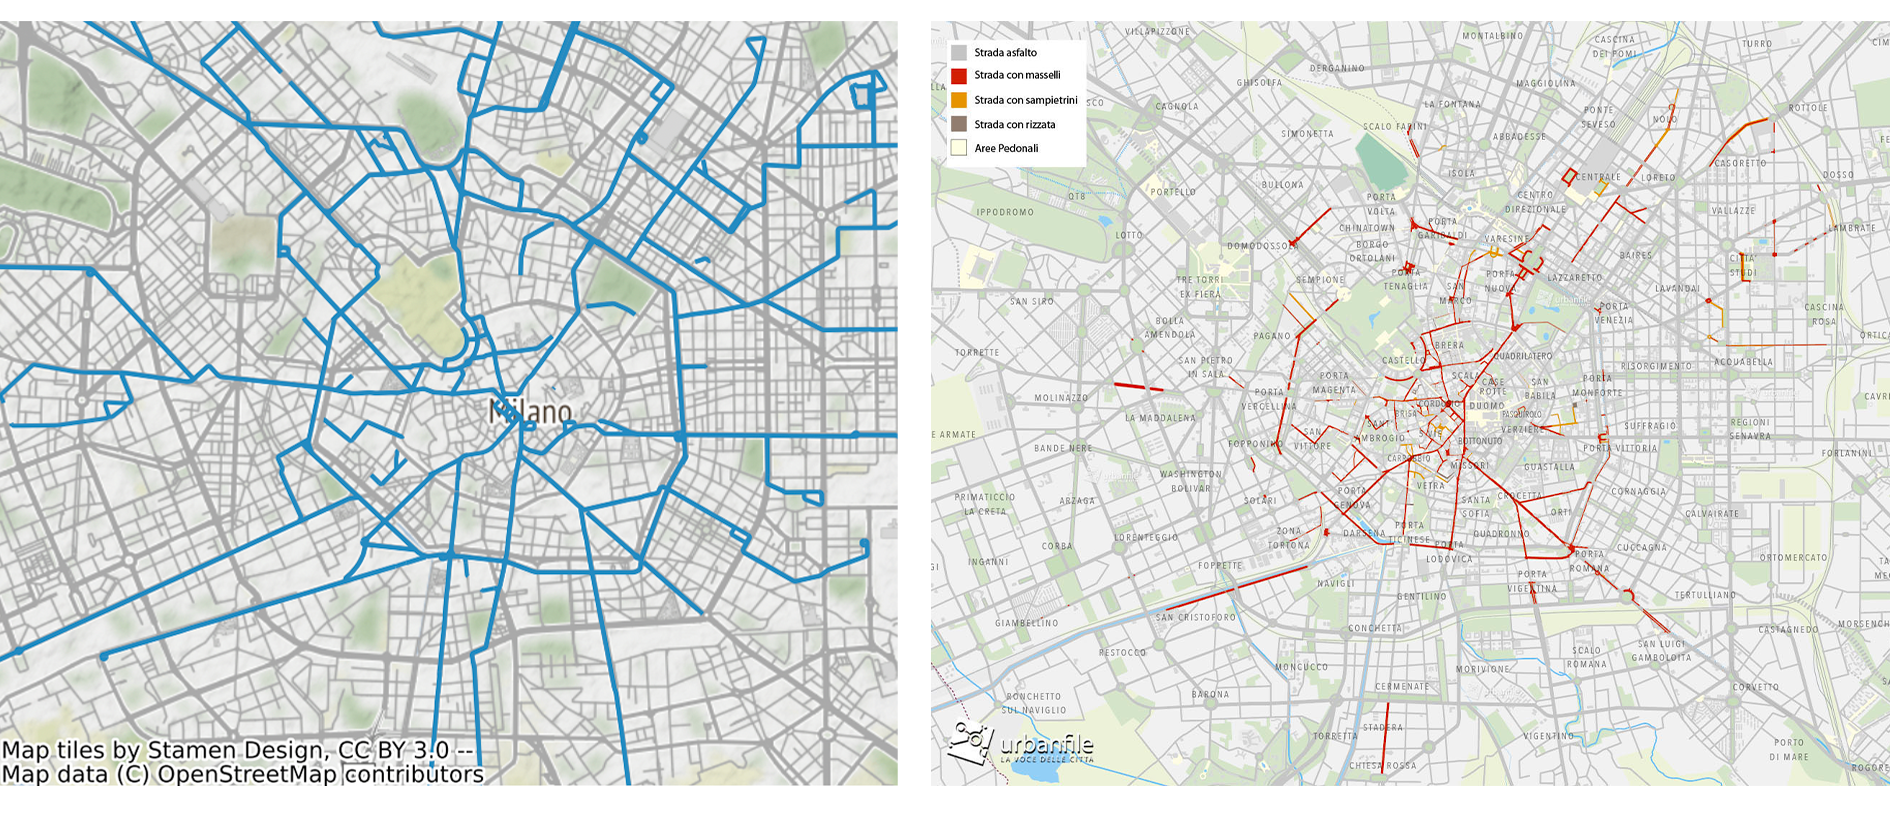
\includegraphics[width=0.48\linewidth]{../src/tram/tram_milano.png}
    \includegraphics[width=0.52\linewidth]{../dataset/pave/Cartina_Milano_Strade_Pavimentazione_Pavé_2.jpg}
    \caption{Cartina con strade in pavè e linee tranviarie a Milano}
    \label{fig:tram-pave-milano}
\end{figure}

\'E possibile notare alcune somiglianze, come per esempio viale Sabotino e via Alessandro Mazoni, 
tuttavia la maggior parte delle linee tranviarie segnate passano su asfalto.
Inoltre, in alcuni viali, come viale Premuda, i tram hanno una carreggiata separata, 
che molto probabilmente ha influenza ancora minore sugli incidenti della zona.

Per creare una stima, si sono convertite le vie principali della cartina trovata 
in geojson, il risultato è visibile nella mappa sulla sinistra 
dell'immagine \ref{fig:mappa-pave}.

\begin{figure}
    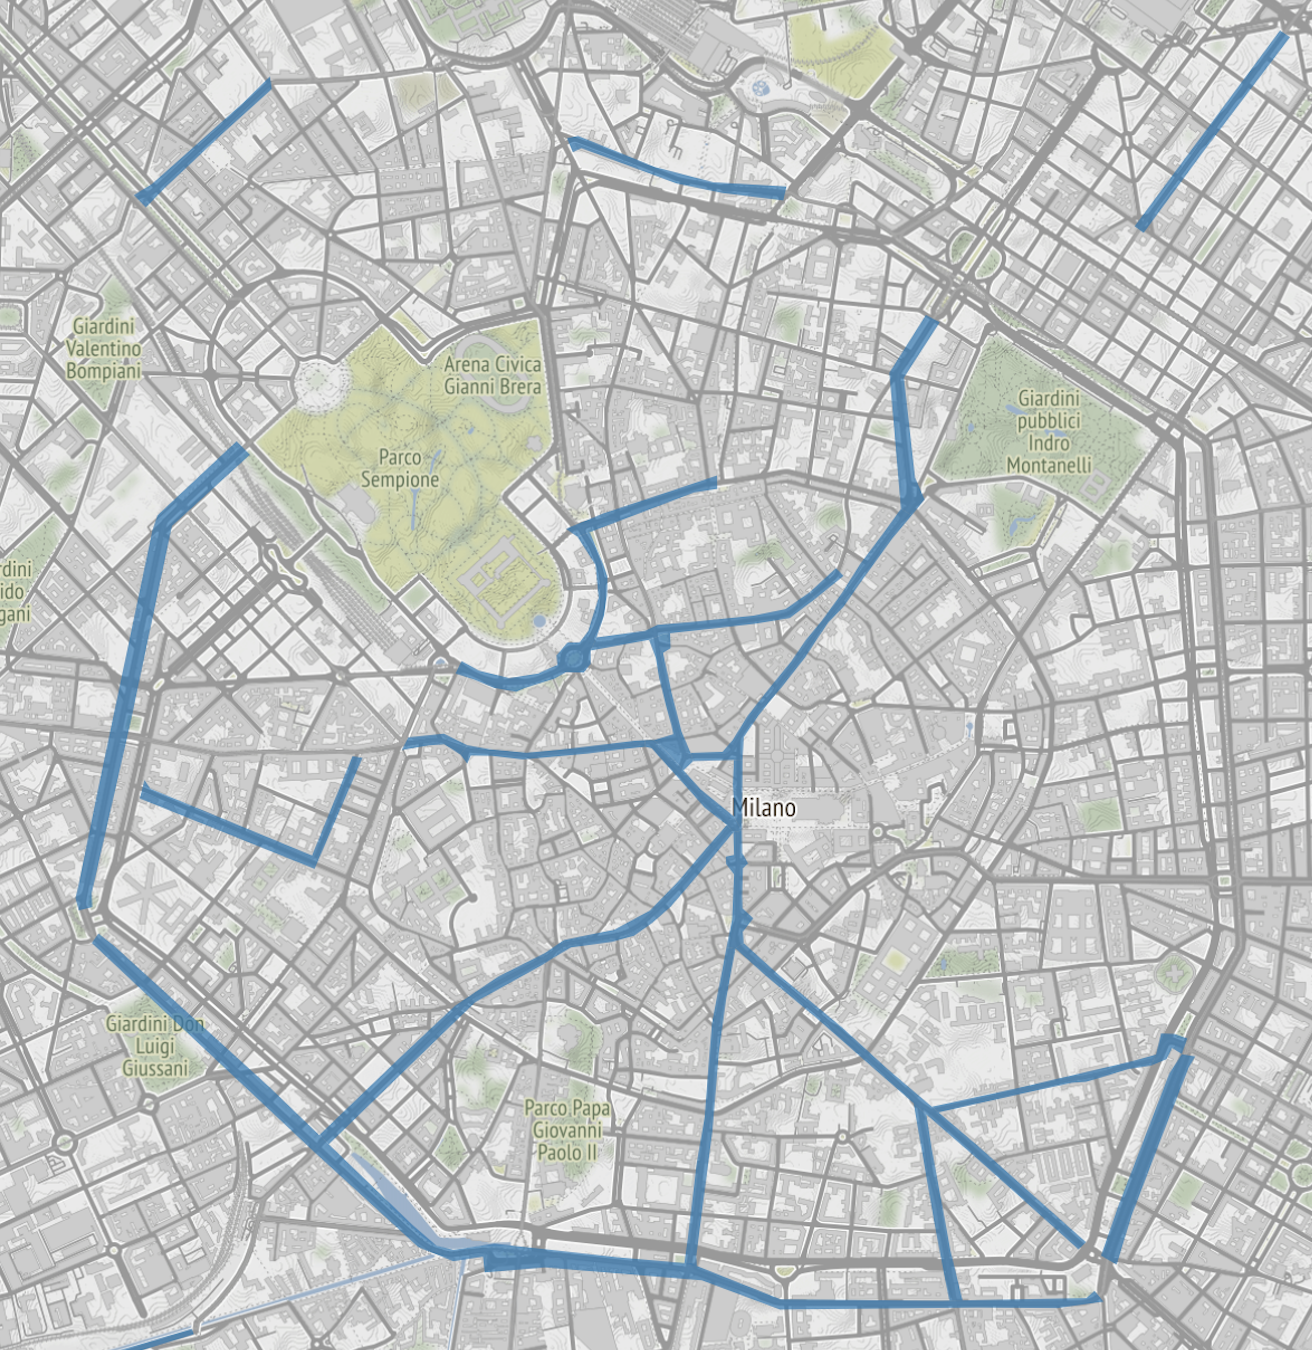
\includegraphics[width=0.5\linewidth]{../src/pave/mappa_pave.png}
    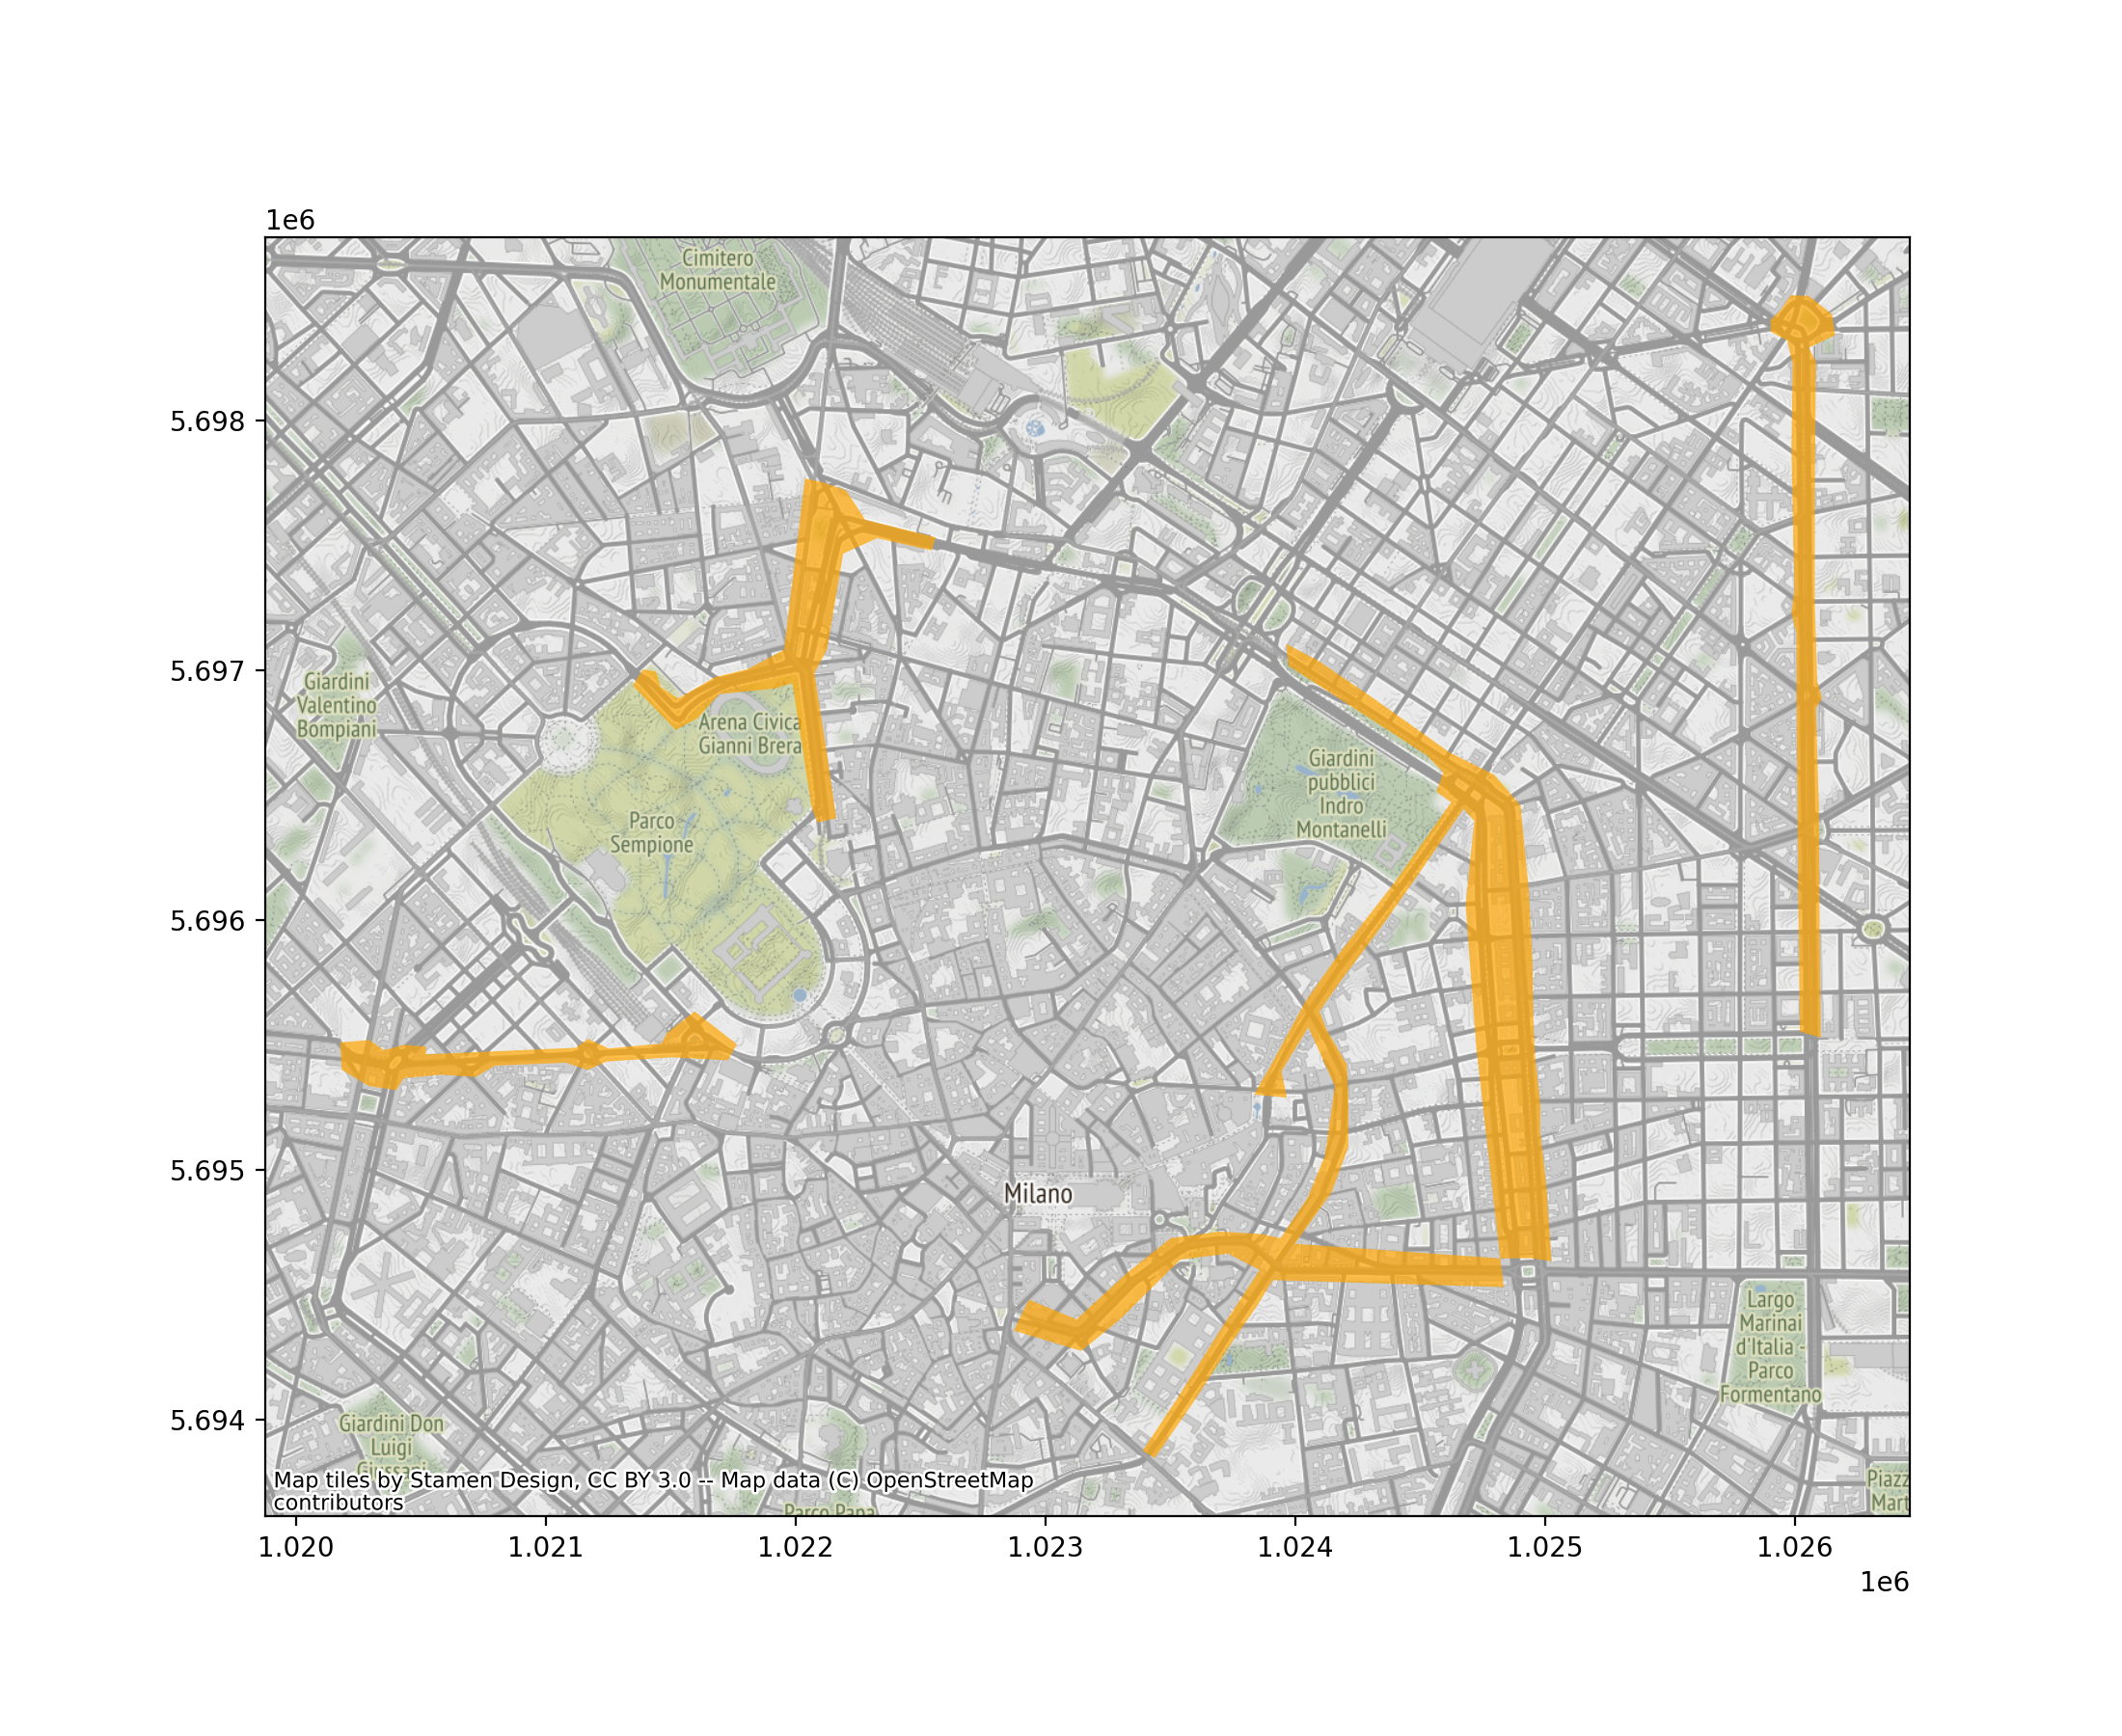
\includegraphics[width=0.5\linewidth]{../src/pave/mappa_asfalto.png}
    \caption{Principali strade a Milano in pavè e campione di strade asfaltate}
    \label{fig:mappa-pave}
\end{figure}

Creata l'area delle strade in pavè, è possibile calcolare quanti sono gli incidenti che 
avvengono in queste zone e confrontarlo con il numero di incidenti nelle strade asfaltate.

\begin{lstlisting}
    inc_in_pave = 0
    for rect in pave['geometry']: 
        rect = geometry.Polygon(rect)

        for point in incidenti['geometry']: 
            if rect.contains(geometry.Point(point)): 
                inc_in_pave += 1

    area_pave = 0
    for rect in pave['geometry']: 
        area_pave += geometry.Polygon(rect).area

    incidenti_per_km = inc_in_pave * 10**6 / area_pave
\end{lstlisting}

Il numero di incidenti per chilometro quadrato, nelle strade in pavè è  $229.45$, che è un valore 
particolarmente alto, anche se viene confrontato con il numero di incidenti nel centro storico, 
cioè circa 130.
Tuttavia, bisogna tenere in considerazione che il dataset che è appena stato creato, contiene solamente 
strade, senza alcuna zona morta, come edifici, mentre l'area utilizzata del centro storico, 
contiene tutto il territorio del centro.

Per ovviare a questo problema, si è creato un campione di strade asfaltate, prese circa 
nella stessa zona di Milano. 
Queste strade sono raffigurate nella mappa destra in figura \ref{fig:mappa-pave}. 
Si è inoltre tentato di tenere i due campioni di strade il più simili possibili, sia per zona, 
sia per area totale del dataset.

Eseguendo lo stesso calcolo realizzato per le strade in pavè, risulta che il numero di incidenti per 
chilometro quadrato, nel campione creato, sia di $220.89$ incidenti.
Tuttavia, nel campione delle strade asfaltate sono stati presi vari tratti provenienti dalla 
circonvallazione interna e altre zone molto trafficate, mentre il campione di strade in pavè 
contiene, per mancanza di altri dati, molte strade del centro storico inevitabilmente 
meno trafficate.

%\clearpage
\section{Incidenti e Autovelox}

Per sapere se gli autovelox hanno influenza sull'incidentalità, 
bisognerebbe innanzi tutto sapere quando sono stati posizionati i dispositivi, e solo a quel punto, 
avendo dati su incidenti prima e dopo l'installazione, sarebbe possibile trarre conclusioni.

Alcuni dati sull'installazione di autovelox esistono per l'anno 2014, visualizzabili nella 
tabella \ref{ztl-milano}, tuttavia le posizioni degli incidenti 
sono solo disponibili per l'anno 2016, in quanto Istat non ha rilasciato 
le posizioni degli incidenti in altre annate.

Conoscendo le posizioni degli autovelox installati nel 2014, è possibile ricondursi alla 
posizione effettiva di questi ultimi sulla mappa.
Per fare ciò, la soluzione più veloce è stata quella di enumerare, 
come raffigurato nella mappa sul lato sinistro della figura \ref{fig:autovelox-indici}, 
tutti gli autovelox, e confrontarli con le vie della tabella.

\begin{lstlisting}[language=Python]
    path = "dataset/autovelox/autovelox_milano.geojson"
    autovelox = gp.read_file(path).to_crs(epsg=3857)
    layer_autovelox = autovelox.plot(figsize=(11,9), color="red")
    
    index = 0
    for lat, lon in geo_utils.parse_geojson_point_list(autovelox['geometry'].astype(str)):
        layer_autovelox.text(lat, lon, s=index)
        # si aggiunge un label per ogni punto
        index += 1
    
    cx.add_basemap(ax=layer_autovelox)
    plt.show()
\end{lstlisting}

\begin{figure}
    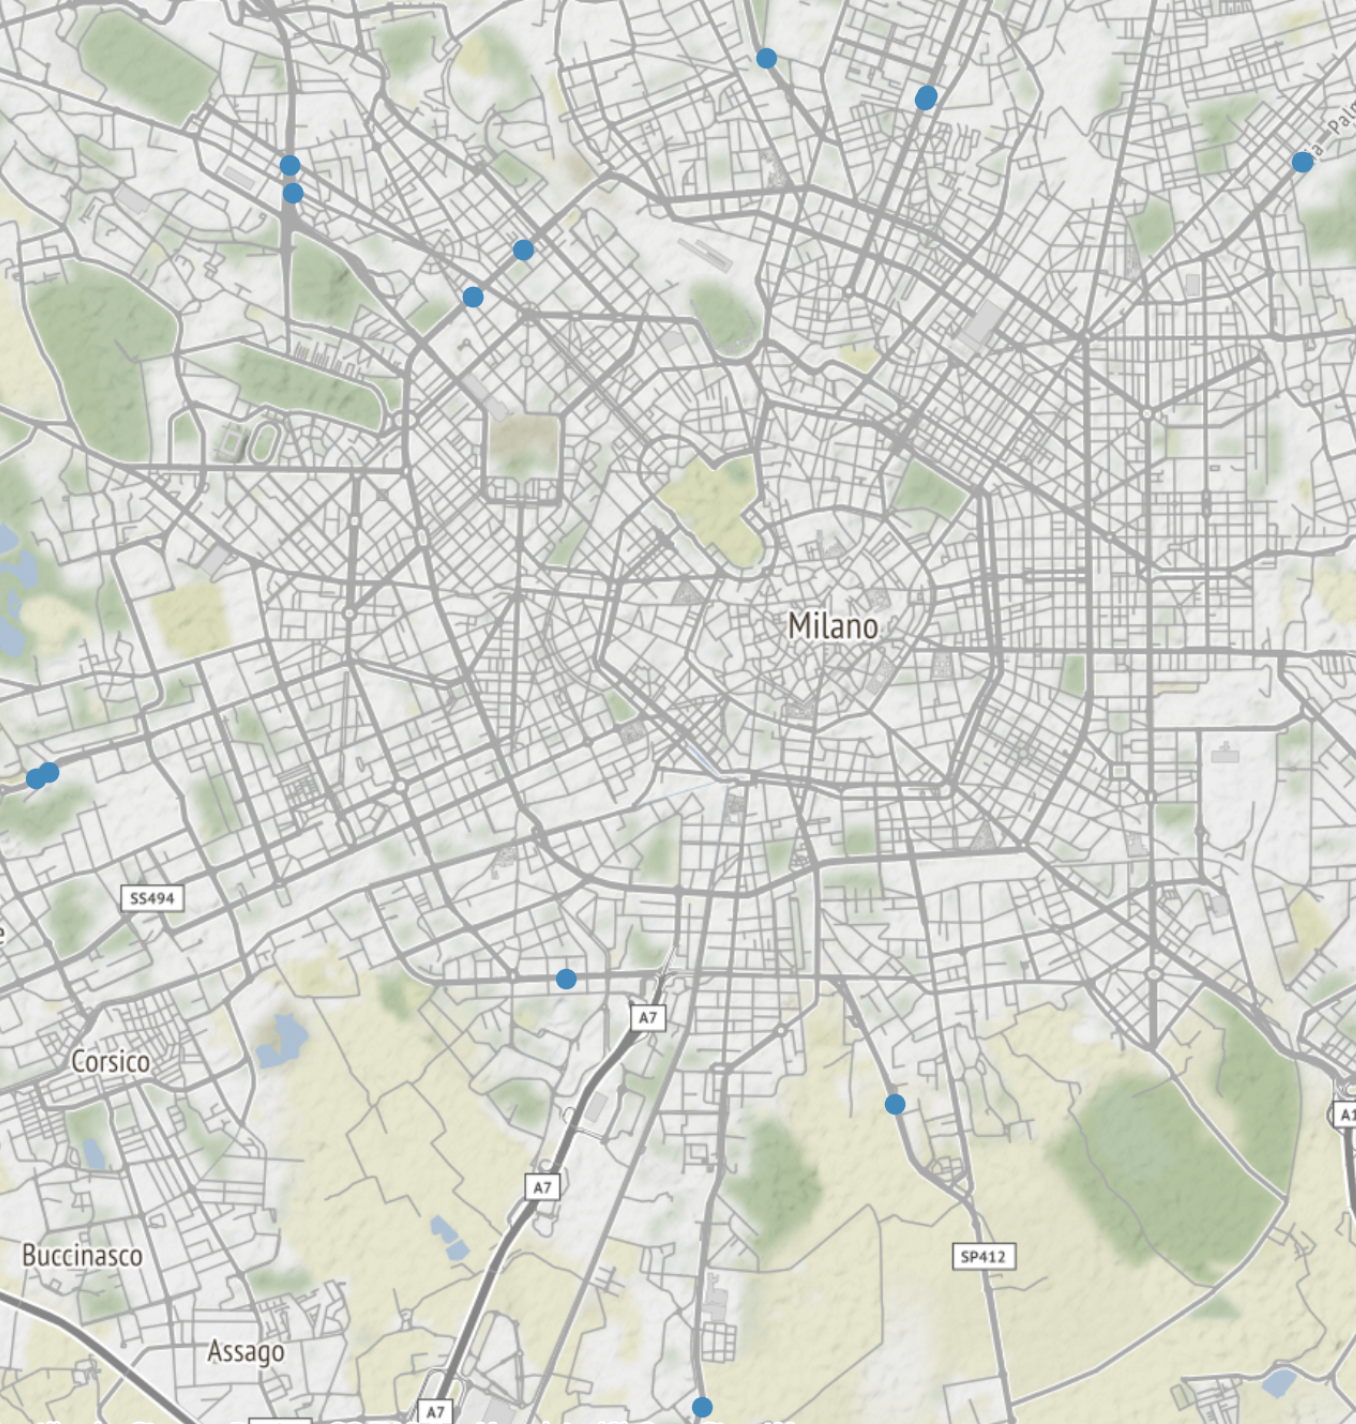
\includegraphics[width=\linewidth]{../src/autovelox/autovelox_2014.png}
    \caption{Autovelox installati nel 2014 e quelli il cui anno di installazione è ignoto}
    \label{fig:autovelox-indici}
\end{figure}

Una volta identificate le linee riguardanti gli autovelox interessati, è possibile separarli 
dal dataset completo.
Gli autovelox installati nel 2014, sono rappresentati nella mappa in 
figura \ref{fig:autovelox-indici}.

Per quanto non si disponga delle informazioni sugli incidenti prima e dopo dell'installazione, 
è comunque possibile sovrapporre i dataset, per vedere se gli autovelox hanno un qualche tipo di 
effetto sugli incidenti, visto che i dati sui sinistri sono successivi all'installazione delle centraline.

\begin{figure}
    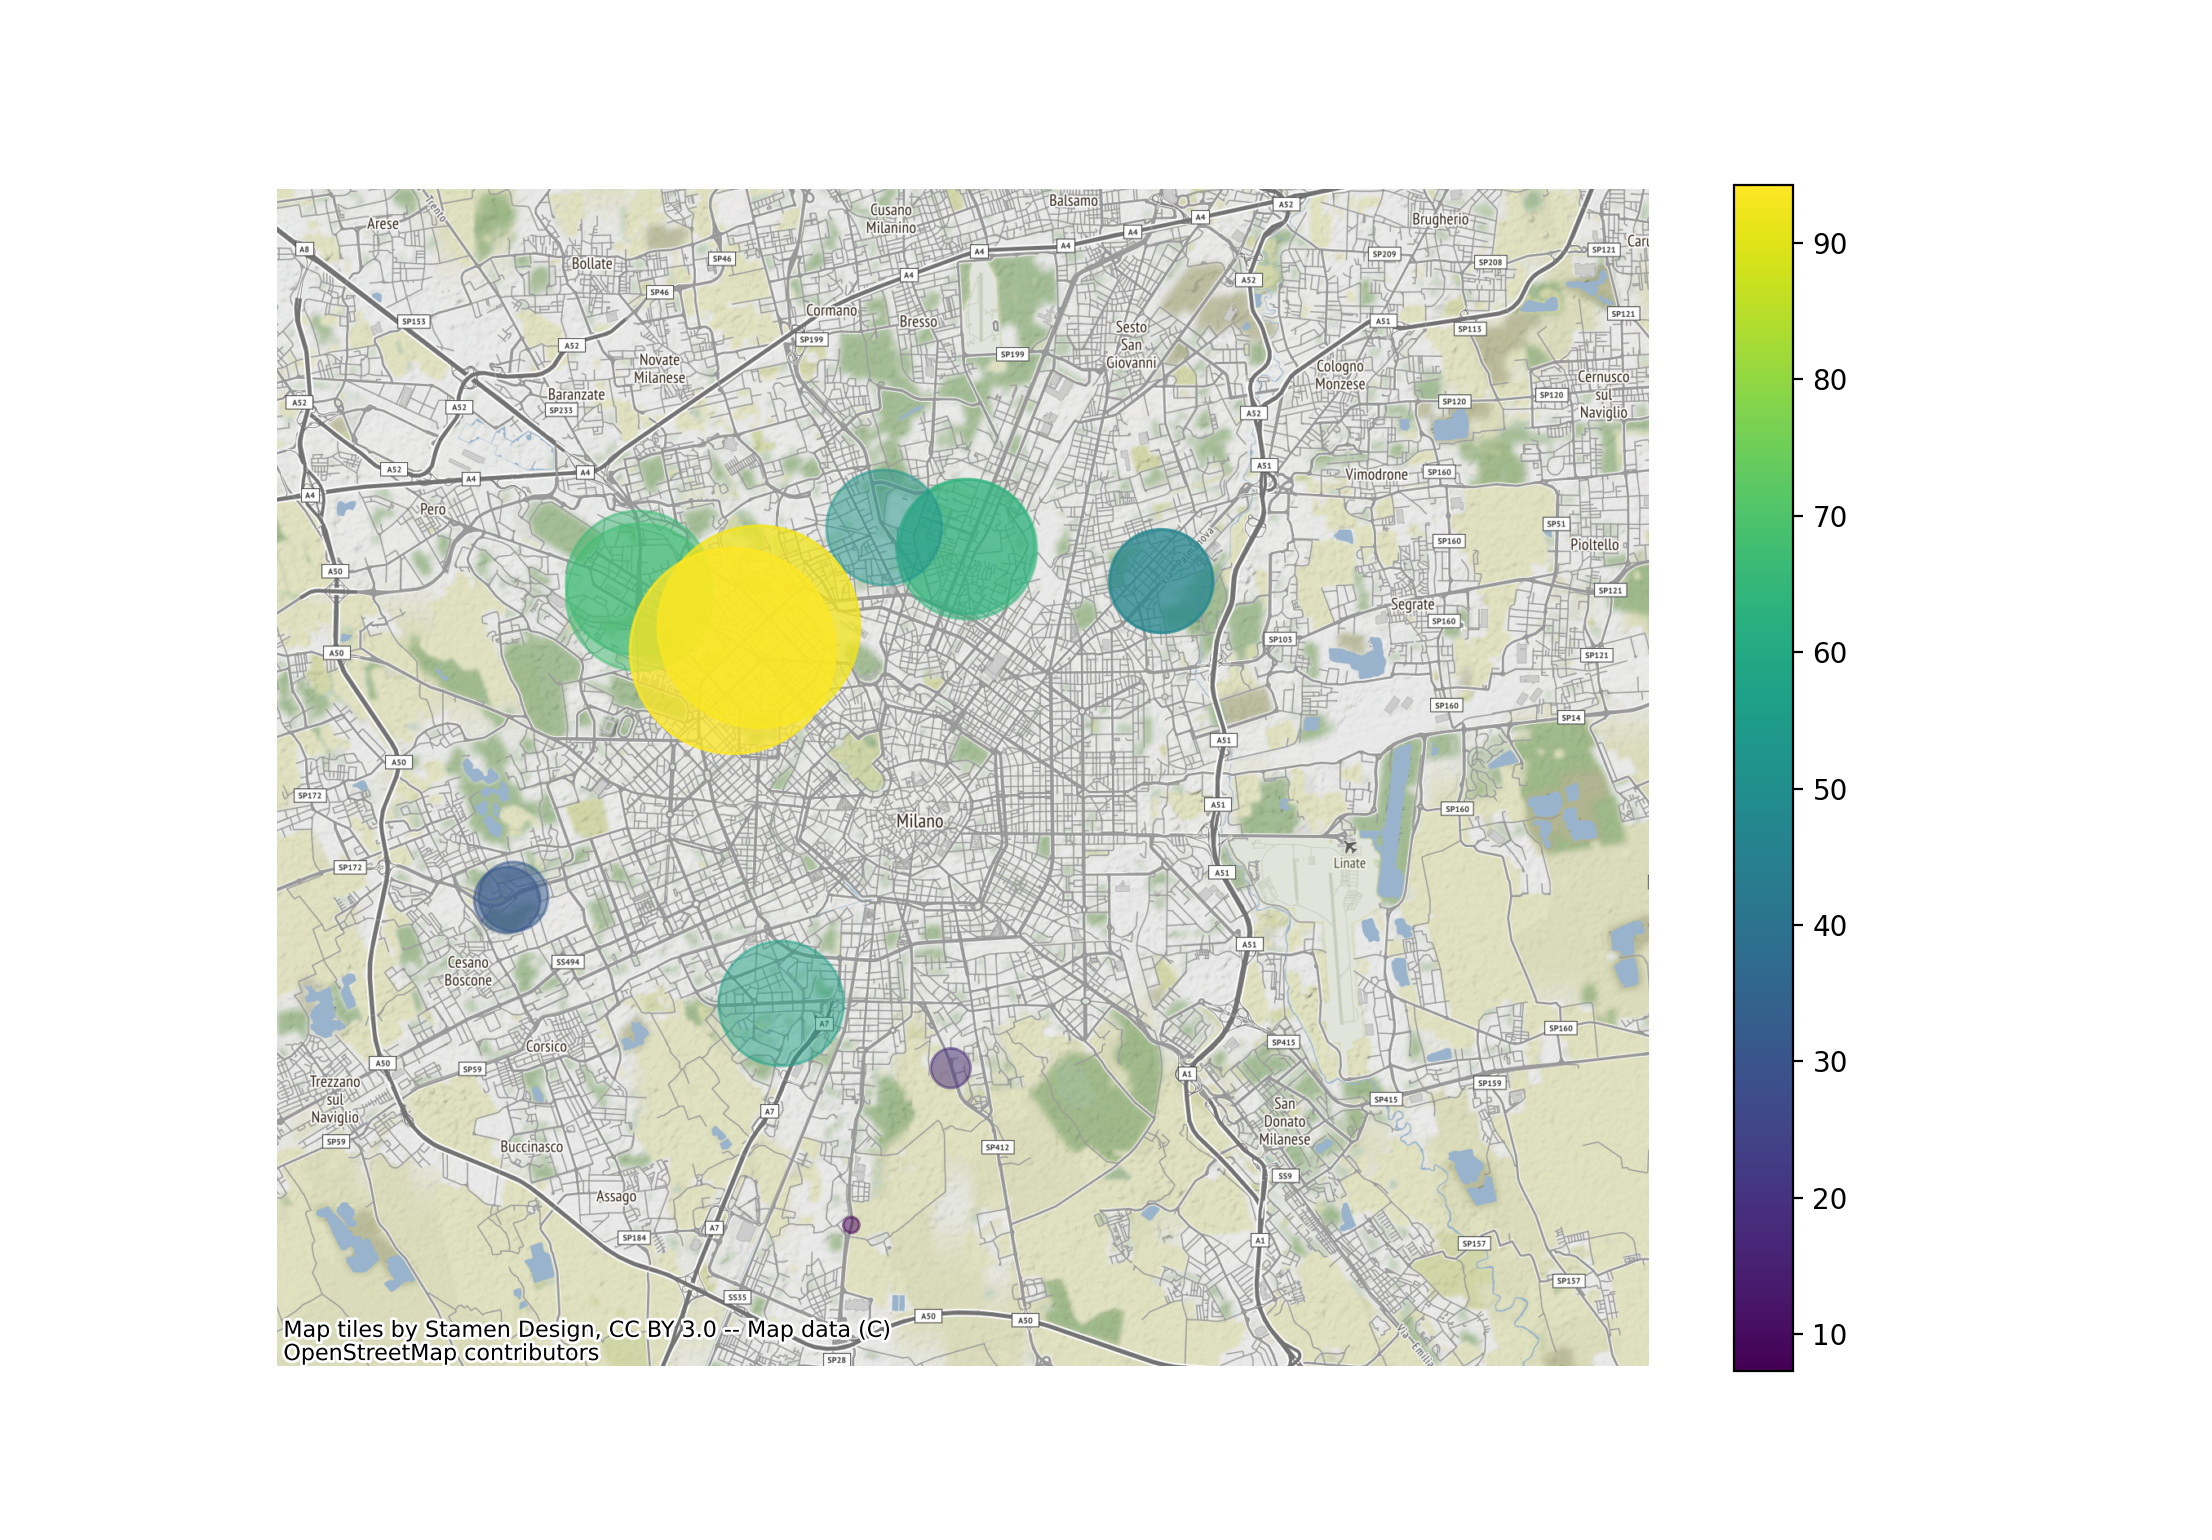
\includegraphics[width=\linewidth]{../src/autovelox/autovelox_incidenti.png}
    \caption{Autovelox e Incidenti a Milano}
    \label{fig:autovelox-incidenti}
\end{figure}

La mappa \ref{fig:autovelox-incidenti} è stata realizzata contando gli incidenti avvenuti 
nel raggio di un chilometro a ogni autovelox.
Va precisato che le \quotestyle{bolle} non indicano il raggio di conteggio degli incidenti, ma 
il numero dei sinistri trovati. La colorazione delle \quotestyle{bolle} è stata aggiunta per 
rendere il grafo più leggibile, la cui interpretazione poteva essere difficoltosa 
osservando solo l'ampiezza dei cerchi.

\begin{center}
    \def\arraystretch{1.5}% 
    \begin{tabular}{ |c|c|c|c| }
        \hline
        Autovelox & Inc. Totali & Inc. per $Km^2$ & Inc. per zona \\ 
        \hline
        \rowcolor{TableGray}
        V. F. Testi d. perif.\footnotemark[1]   &   194 &   61.78   &   69.52 \\
        V. F. Testi d. centro                   &   202 &   64.33   &   69.52 \\
        \rowcolor{TableGray}
        C. Ghisallo d. centro\footnotemark[2]   &   208 &   66.24   &   44.3 \\
        C. Ghisallo d. perif.                   &   212 &   67.51   &   44.3 \\
        \rowcolor{TableGray}
        V. Fermi                                &   166 &   52.86   &   51.25 \\
        V. Parri d. perif.                      &    95 &   30.25   &   43.63 \\
        \rowcolor{TableGray}
        V. Parri d. centro                      &   100 &   31.84   &   43.63 \\
        V. Famagosta                            &   180 &   57.32   &   43.63 \\
        \rowcolor{TableGray}
        V. Missaglia d. centro                  &   23  &    7.32   &   27.54 \\
        V. Ferrari                              &   57  &   18.15   &   44.3 \\
        \rowcolor{TableGray}
        V. Monteceneri d. Serra                 &   291 &   92.67   &   44.3 \\
        V. Monteceneri d. Lugano                &   290 &   92.35   &   44.3 \\
        \rowcolor{TableGray}
        Viale Serra                             &   296 &   94.26   &   44.3 \\
        Viale Serra                             &   296 &   94.26   &   44.3 \\
        \rowcolor{TableGray}
        V. Palmanova d. perif.                  &   149 &   47.45   &   59.79 \\
        V. Palmanova d. centro                  &   149 &   47.45   &   59.79 \\
        \hline
    \end{tabular}
\end{center}

\footnotetext[1]{Viale Fulvio Testi}
\footnotetext[2]{Cavalcavia del Ghisallo}

Una volta trovati gli incidenti totali, è possile calcolare gli incidenti sulla base dell'area 
utilizzata.
Nel seguente codice, al dataset autovelox sono aggiunte due colonne, una contenente gli 
incidenti totali, l'altra contenente gli incidenti per chilometro.

\begin{lstlisting}
    autovelox_2014['incidenti_vicini'] = gp.GeoSeries(df)
    autovelox_2014['incidenti_pesati'] = autovelox_2014['incidenti_vicini'] / 3.14
\end{lstlisting}

Questa ultima colonna, in particolare, è divisa per 3.14 perchè l'area del cerchio è data dalla formula: 

\begin{center}
    $Area\, = \pi * r^2$
\end{center}

Poichè si sta utilizzando raggio di circa un chilometro, e si vuole ottenere il numero di incidenti per chilometro 
quadrato, l'area ottentuta è $3.14$.

Per facilitare la lettura della tabella precedente, nella figura \ref{fig:confronto-autovelox} è visibile il 
confronto tra il numero di incidenti vicino a autovelox, e il numero di incidenti del municipio.

In alcuni casi, il numero di incidenti sembra essere  ridotto dalla presenza dell'autovelox 
tuttavia, nella maggior parte dei casi, e soprattutto nelle zone di Viale Serra e Viale Monteceneri, 
il volume di incidenti è particolarmente più alto di quello del municipio.

\'E possibile che, non avendo dati sufficienti a calcolare una tendenza precedente all'installazione 
dell'autovelox, questa zona sia particolarmente pericolosae non si ha modo di saperlo.

\begin{figure}
    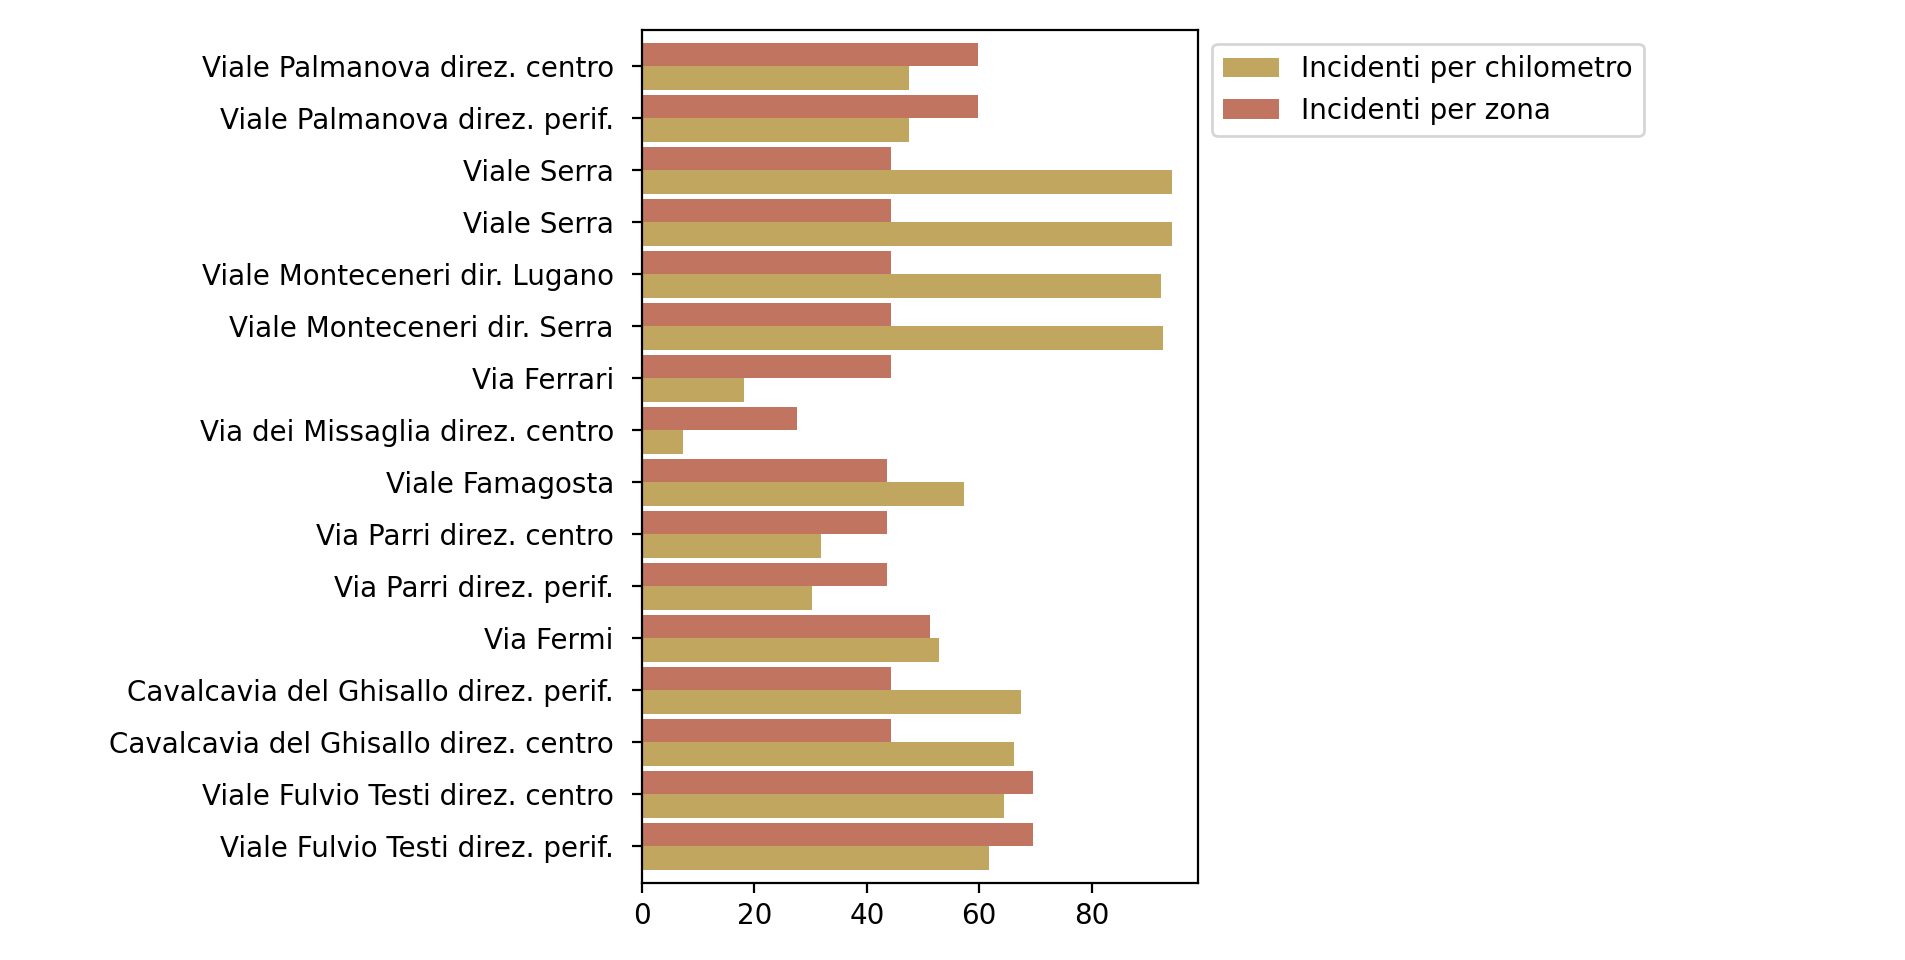
\includegraphics[width=\linewidth]{../src/municipi_milano/conclusioni_municipio.png}
    \caption{Incidenti vicino a autovelox rispetto a quelli per zona di Milano}
    \label{fig:confronto-autovelox}
\end{figure}

\begin{lstlisting}
    incremento_percentuale_totale = 0
    for km, zona in zip(data['Incidenti per chilometro'], data['Incidenti per zona']): 
        incremento_percentuale = (km - zona) * 100 / zona
        incremento_percentuale_totale += incremento_percentuale

    print(incremento_percentuale_totale)
\end{lstlisting}

Con i dati che si hanno a disposizione, è possibile calcolare l'incremento (o decremento), degli 
incidenti in zone vicine a autovelox.
A causa delle zone menzionate in precedenza, in vicinanza di autovelox si ha un incremento degli 
incidenti del $329.6$\%, tuttavia, nel caso in cui si considerino 
outlier\footnote{In un campione di osservazioni, un outlier è un valore anomalo, 
particolarmente distante dagli altri dati disponibili \cite{PROB_E_STATISTICA:1}} 
i Viali Serra e Monteceneri, si ha invece un decremento generale del $113.6$\%.


%%%%%%%%%%%%%%%%%%%%%%%%%%%%%%%%%%%%%%%%%%%%%%%%%%%%%%
%\clearpage
\chapter{Dati su Incidenti}

Per quanto riguarda dati generali su incidenti in Italia, sono disponibili due dataset molto ampi. 
Il primo, rilasciato da Istat, contiene campi come data, ora, 
numero di persone a bordo, tipo di incrocio e tipo di veicolo.
Queste informazioni sono presenti a partire dal 2010 fino al 2018.
Il secondo è invece messo a disposizione da Automobile Club D'Italia (ACI) che contiene dati simili, 
ma in più contiene informazioni sul luogo dell'incidente, come autostrada o strada provinciale.

%\clearpage
\section{Dati Istat su veicoli}

%\clearpage
\subsection{Il tipo di veicolo dipende dalla strada?}

Sarebbe interessante sapere quanto la composizione del traffico, per quanto riguarda i veicoli, 
cambia al cambiare del tipo di strada.

\begin{lstlisting}[language=Python]
    strade_urbane = data[(data['localizzazione_incidente'] == 1) | (data['localizzazione_incidente'] == 2) | (data['localizzazione_incidente'] == 3)]['tipo_veicolo_a']
    strade_extraurbane = data[(data['localizzazione_incidente'] == 4) | (data['localizzazione_incidente'] == 5) | (data['localizzazione_incidente'] == 6)]['tipo_veicolo_a']

    # Dove 1,2,3 sono gli ID dei diversi tipi di strade urbane, 
    # mentre 4,5,6 gli ID delle strade extraurbane
\end{lstlisting}

Il grafo \ref{fig:differenza-strade} rappresenta quali sono le categorie di veicoli coinvolte 
con più frequenza in sinistri, per tre tipi di strade diverse. 
Le percentuali sono calcolate per gruppo, quindi sommando 
tutte le righe di, per esempio Autostrade, si ottiene $1.0$.

Nonostante le auto private siano di gran lunga il tipo di veicolo 
più coinvolto in incidenti, nelle autostrade non sono presenti molti incidenti con motocicli, 
mentre cresce molto il numero di questi nelle strade urbane.

\begin{figure}
    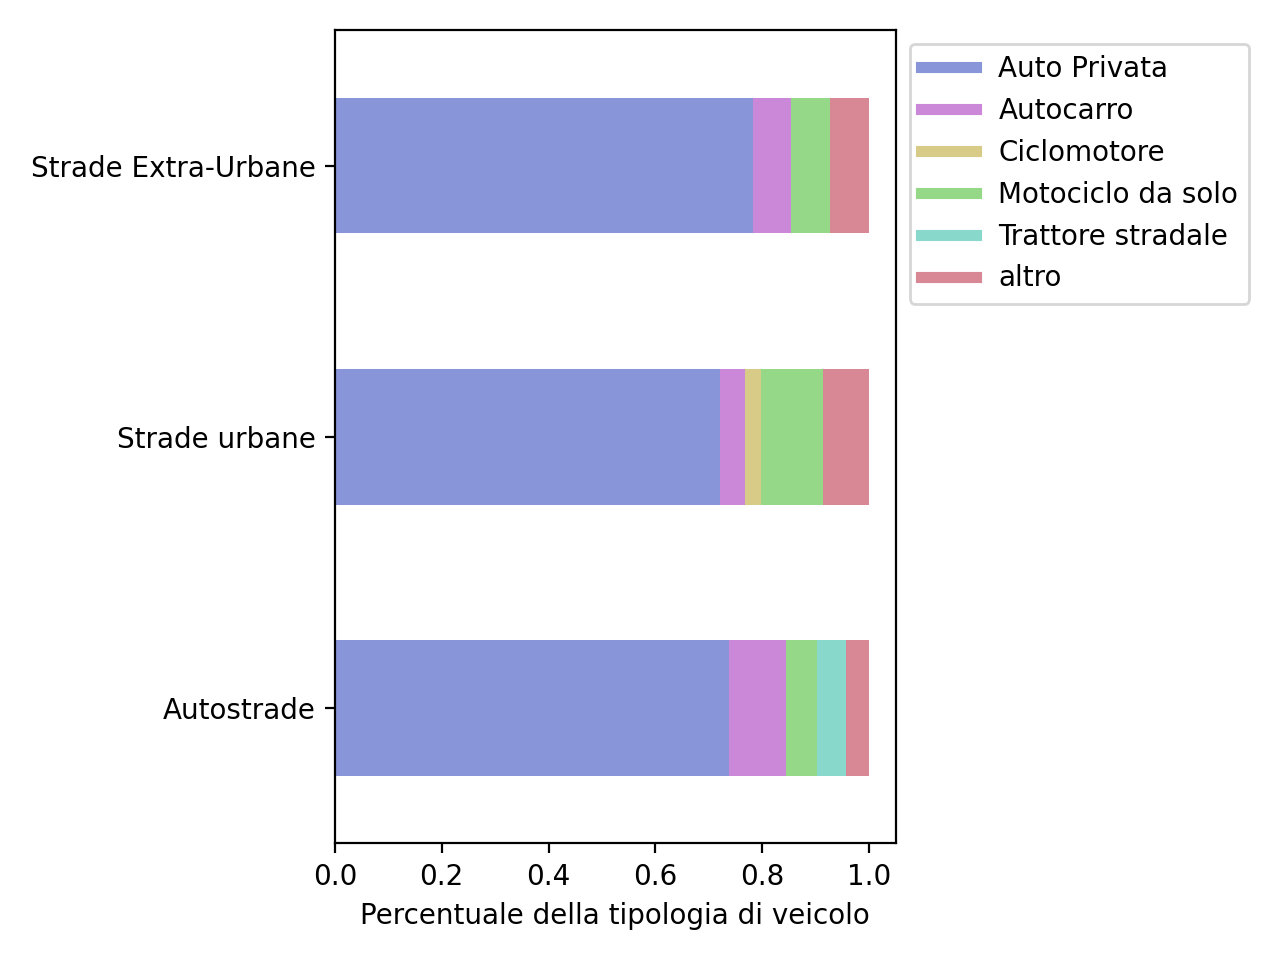
\includegraphics[width=\linewidth]{../src/incidenti/incidenti_senza_coords/tipo_veicoli/differenza_strade.png}
    \caption{Incidenti per tipo di veicolo nel 2018}
    \label{fig:differenza-strade}
\end{figure}

Visto che le auto private causano oltre tre quarti degli incidenti in ogni categoria di strada,  
si è deciso di ometterle, per controllare la presenza di differenze nelle altre tipologie 
di veicoli.
I risultati sono rappresentati, per l'anno 2018, nella figura \ref{fig:differenza-strade-no-auto}.

\begin{figure}
    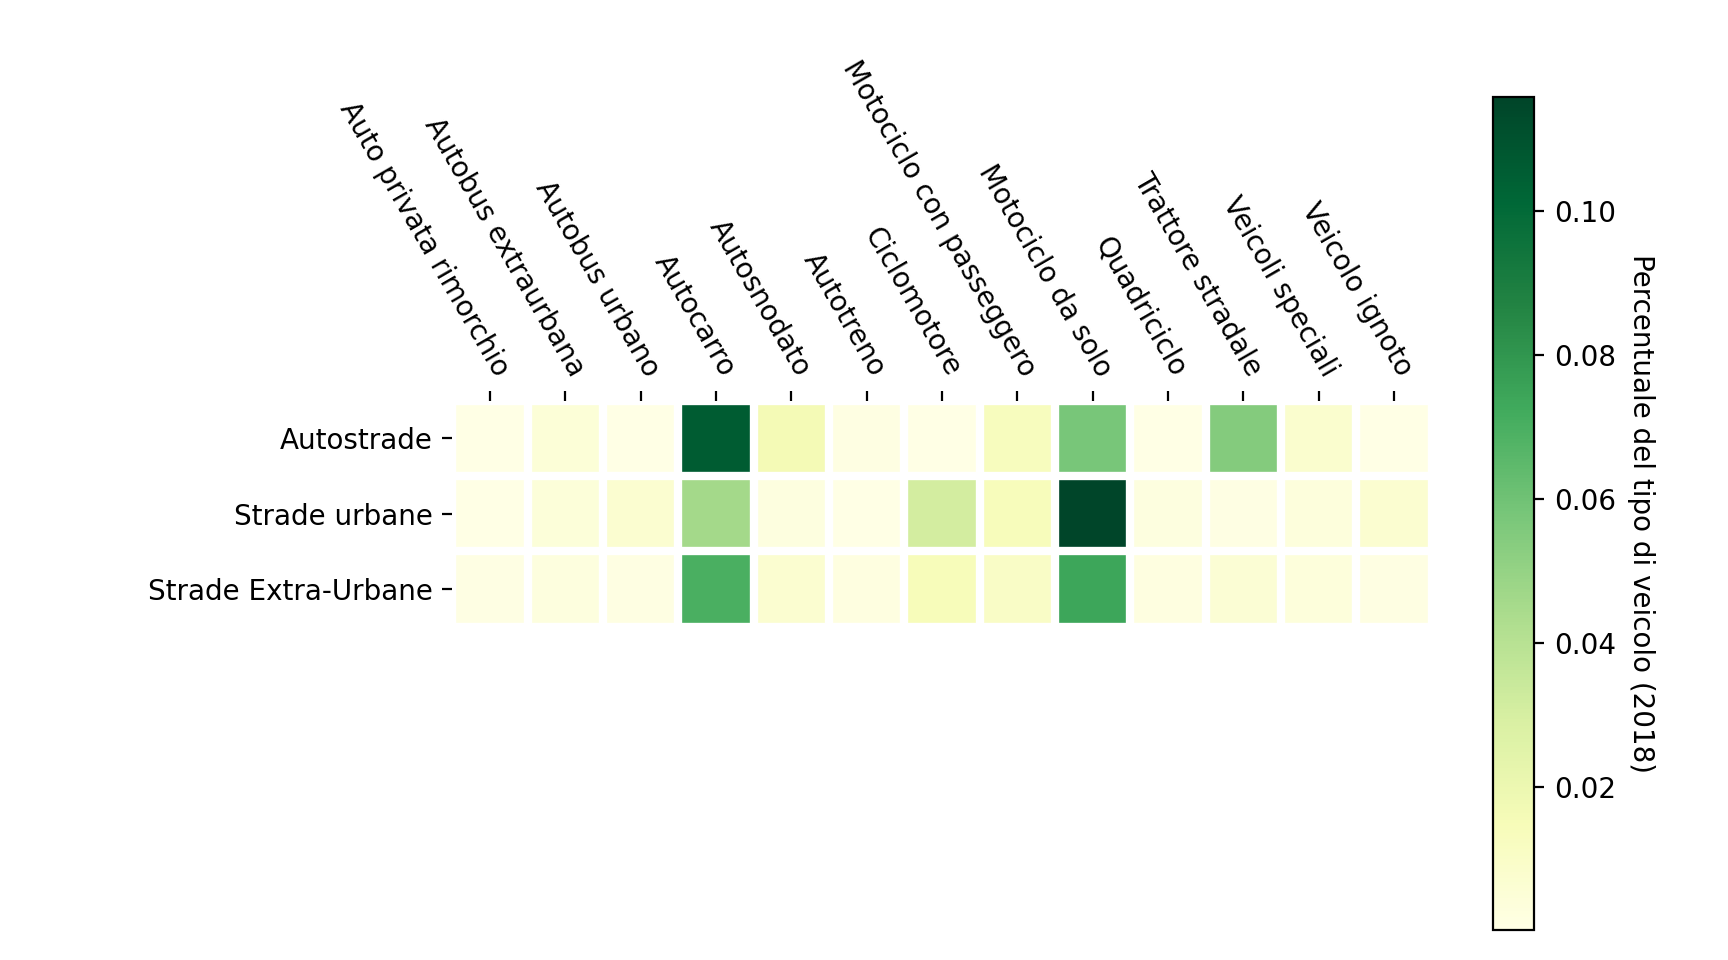
\includegraphics[width=\linewidth]{../src/incidenti/incidenti_senza_coords/tipo_veicoli/differenza_senza_auto.png}
    \caption{Incidenti per tipo veicolo, senza contare le auto private}
    \label{fig:differenza-strade-no-auto}
\end{figure}

Omesse le automobili private, appare chiaro che gli autocarri sono coinvolti in un maggior 
numero di incidenti su autostrade, mentre i motocicli il primato sulle strade urbane.
Può anche sembrare strano che i trattori stradali siano coinvolti così spesso in incidenti 
su autostrade, tuttavia, in questo caso, per 'trattore' non si intende la macchina 
agricola, ma la motrice di un autocarro.

Va comunque sottolineato che le percentuali di incidenti provocati da queste tipologie di 
veicoli, sono tutte al di sotto del $10$\%.

%\clearpage
\section{Dati Istat su conducente}

%\clearpage
\subsection{Esistono differenze tra la guida di un uomo e quella di una donna?}

\begin{figure}
    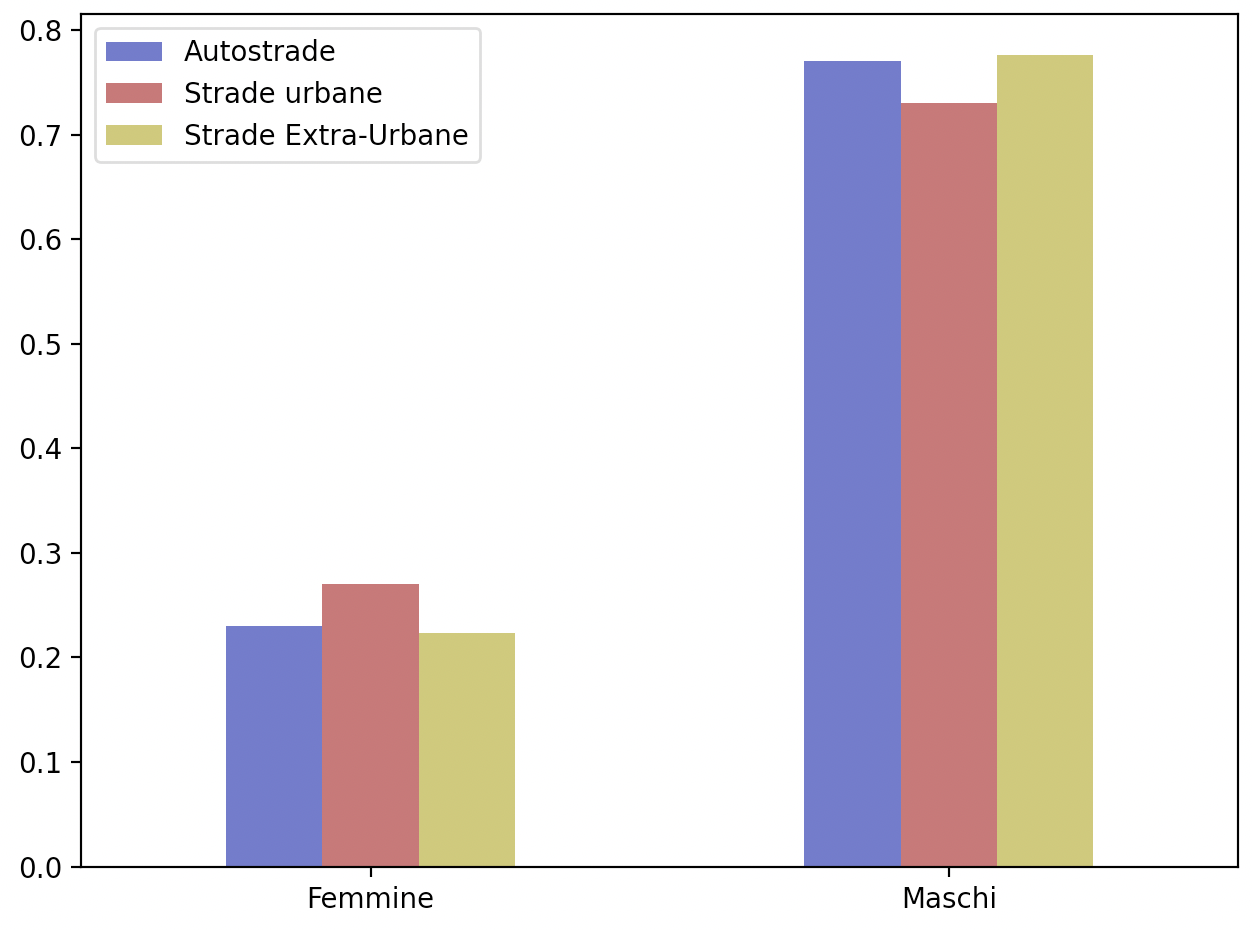
\includegraphics[width=\linewidth]{../src/incidenti/incidenti_senza_coords/tipo_veicoli/uomo-donna.png}
    \caption{Sesso del conducente per tipo di veicolo nel 2018}
    \label{fig:differenza-uomo-donna}
\end{figure}

Il grafo \ref{fig:differenza-uomo-donna} mostra che non c'è molta differenza tra i vari tipi di 
strada, per quanto riguarda il sesso del coducente.\\
Il numero di incidenti per genere è tende ad essere 75\% circa uomini e 25\% donne.
Nelle strade  urbane, la percentuale di incidenti con conducente donna aumenta leggermente nel 2018, 
questo vale per tutti gli anni?

\begin{center}
    \def\arraystretch{1.5}% 
    \begin{tabular}{ |c|c|c|c| }
        \hline
        Anno & Sesso & Autostrade & Strade Urbane \\ 
        \hline
        \rowcolor{TableGray}
        2018 & Uomo & 77\%  & 73\% \\
        2018 & Donna & 23\% & 27\% \\
        \rowcolor{TableGray}
        2016 & Uomo & 75.8\%  & 71.9\% \\
        2016 & Donna & 24.2\% & 28.1\% \\
        \rowcolor{TableGray}
        2014 & Uomo & 74.2\%  & 70.7\% \\
        2014 & Donna & 25.8\% & 29.3\% \\
        \hline
    \end{tabular}
\end{center}

In tutti gli anni la percentuale di uomini e donne coinvolti in incidenti è consistente, 
questo fenomeno fa sospettare che ci siano più uomini al volante rispetto alle donne.
Un modo per testare l'ipotesi è quello di ricavare un campione di conducenti, separando tra 
uomini e donne.
Va sottolineato che un campione, preso durante la pandemia di Covid-19, in un mese di quarantena 
non sarà mai uno stimatore estremamente accurato della percentuale di maschi e femmine al volante.

Si sono, comunque, contati i conducenti delle vetture passanti a Somma 
Lombardo\footnote{sul Sempione basso, strada urbana principale, all'altezza chiesa di San Bernardino}, 
tra le 15 e le 16 di Giovedì 5 Novembre 
(settimana predente alla seconda chiusura della Lombardia), 
sono stati ottenuti i seguenti risultati:

\begin{center}
    \def\arraystretch{1.5}% 
    \begin{tabular}{ |c|c|c| }
        \hline
        Sesso & Numero & Percentuale \\ 
        \hline
        \rowcolor{TableGray}
        Uomini & 483 & 68.8\% \\
        Donne & 219 & 31.2\% \\
        \hline
    \end{tabular}
\end{center}

La percentuale di uomini e donne al volante è equivalente a quella degli incidenti.
Questo dato rafforza l'idea che non esistano differenze sostanziali tra la guida di 
maschi e femmine.

%\clearpage
\subsection{Il numero di passeggeri influisce sull'incidentalità?}

\begin{figure}
    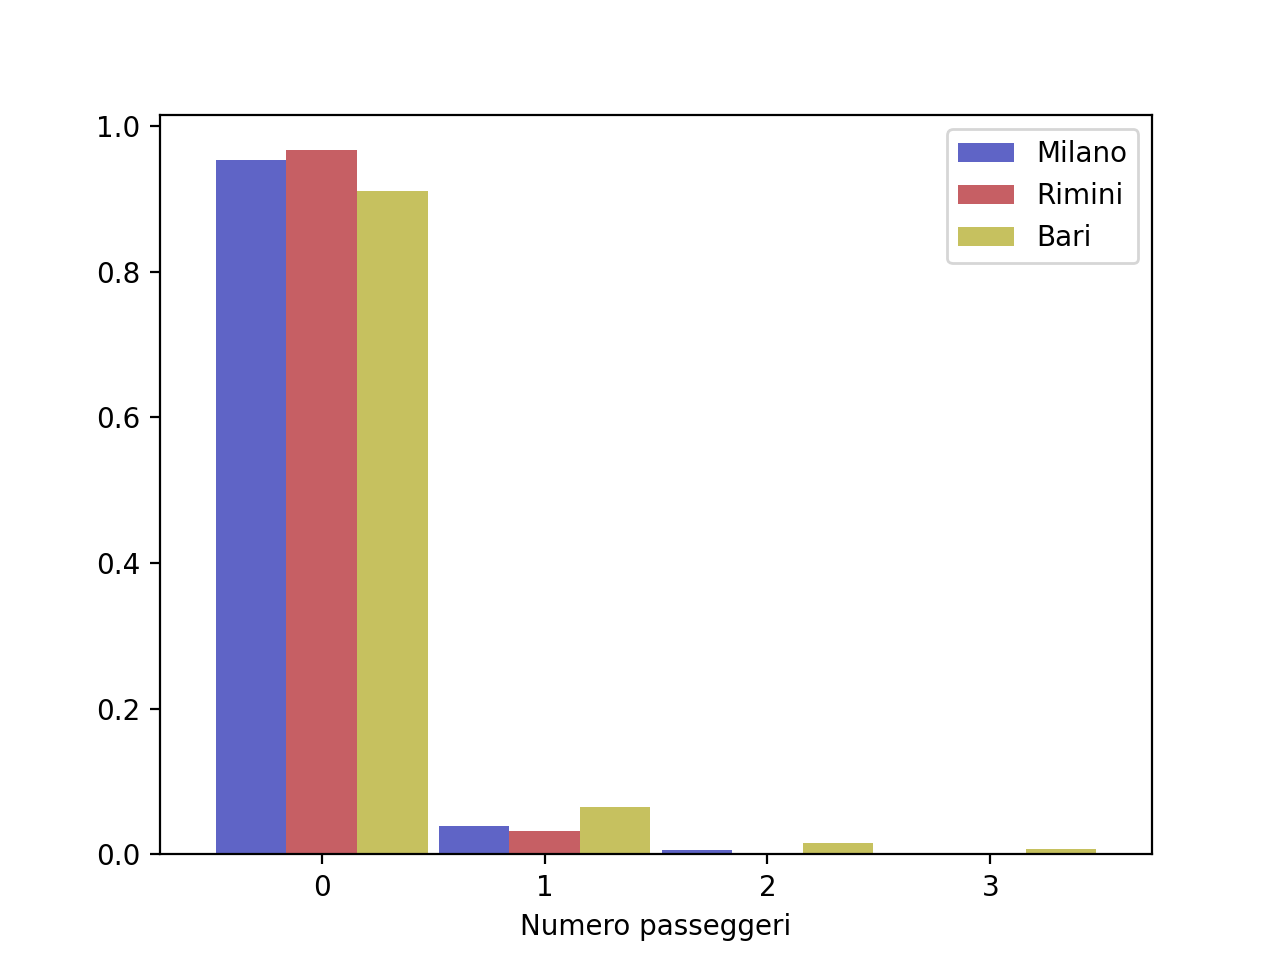
\includegraphics[width=\linewidth]{../src/incidenti/incidenti_senza_coords/passeggeri/passeggeri.png}
    \caption{Numero di passeggeri in incidenti per Milano, Rimini e Bari}
    \label{fig:passeggeri-milano-rimini}
\end{figure}

La figura \ref{fig:passeggeri-milano-rimini} mostra che oltre il 90\% degli incidenti
avviene quando in macchina è presente solo il conducente, cioè la colonna indicata con 0.
Si sono prese in considerazione le provincie di Milano, Rimini e Bari, 
per controllare se la località marittima influisse sul numero di incidenti, 
ma sembra che quest'ultima abbia una percentuale 
ancora più alta di incidenti in cui è presente solo il conducente, rispetto a Milano.

La domanda che sorge spontanea è, se avvengano più incidenti dove è presente 
solo il conducente per il numero frequente di automobili con una sola persona a 
bordo, o per fattori esterni che portano il conducente a distrarsi?

Sarebbe dunque utile poter ricavare un campione di automobili divise per numero 
di persone a bordo. 
Tuttavia, in periodo di Covid-19, una stima di questo tipo non sarà mai accurata.

Nel 2010 in un articolo per la campagna 
Sbilanciamoci!\footnote{https://sbilanciamoci.info/chi-siamo/}, 
Anna Donati scriveva \cite{SBILANCIAMOCI:1}: 

\begin{center}
    \quotestyle{Infatti l’auto passa dal} $59.3$\% \quotestyle{degli spostamenti nel 2000 al $65.3$\% del }
    \quotestyle{2009 e di questi ben il} $57.7$\% 
    \quotestyle{viaggia solo.}
\end{center}

\'E possibile dunque ipotizzare che la percentale di conducenti che viaggiano 
da soli sia approssimativamente attorno al $60$\%, perlomeno nel 2010.
Per realizzare una stima, è necessario conoscere le percentuali di automobili con uno, 
due o tre passeggeri, non presenti nell'articolo e che se esistessero, sarebbero 
valide per l'anno 2010, e non per le annate più recenti.

Ipotizzando però, che il numero di automobili con solo conducente rimangano attorno al 
$60$\%, deve esistere qualche fattore che alza gli incidenti senza passeggeri a 
$95.3$\%.
Uno di questi fattori, che potrebbero distrarre il conducente, deve essere l'utilizzo 
del cellulare nell'automobile.

Va specificato che la fonte di questo articolo è il sito 
Isfort\footnote{https://www.isfort.it/}, in particolare il 
rapporto sulla mobilità.
Sul loro sito, non è più reperibile il rapporto del 2010, tuttavia sono disponibili 
quelli più recenti, in particolare per 
2018\footnote{\url{https://www.isfort.it/wp-content/uploads/2019/09/Rapporto_Mobilita_2018.pdf}}, 
2019, 2020.

%\clearpage
\subsection{L'uso del telefono cellulare ha influenzato il numero di incidenti?}

Non è un segreto che il numero di conducenti che utilizzano lo smartphone alla guida 
è cresciuto negli anni, assieme alla diffusione di quest'ultimo. 
Per il giornale online l'Automobile \cite{AUTOMOBILE:1}, gli automobilisti americani 
passano quasi due minuti guardando il cellulare, per ora di guida.
Questo comportamento non può che influire sull'attenzione alla guida, e di conseguenza 
sul numero di incidenti, sarebbe interessante riuscire a osservare questa tendenza nei 
dati a disposizione.

Per quanto non siano disponibili dati su questo ambito, si potrebbe confrontare gli 
anni tra 2010 e 2013, in cui l'uso del cellulare in macchina ancora non era frequente, 
rispetto agli anni più recenti.

\begin{figure}
    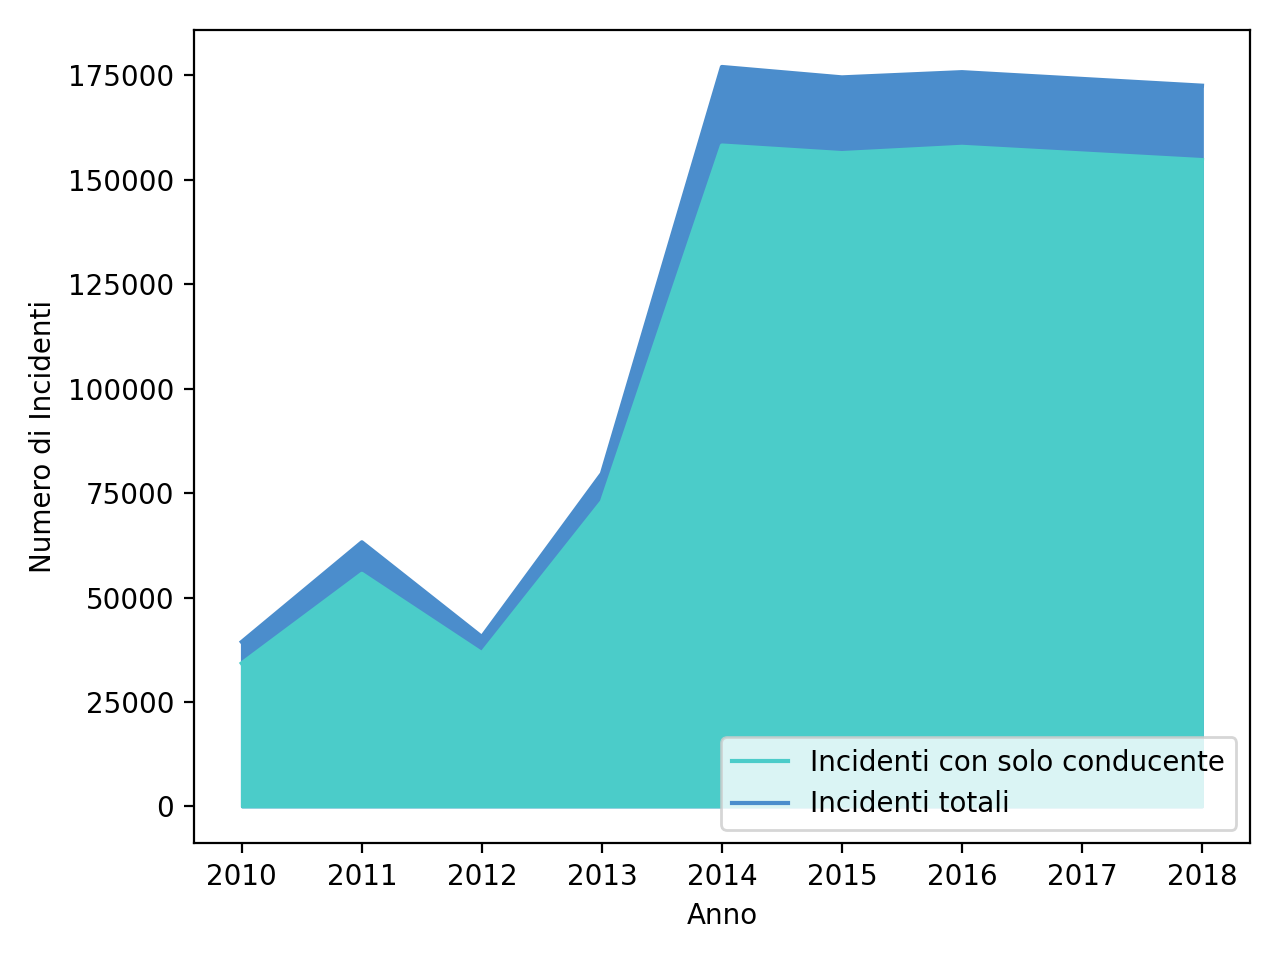
\includegraphics[width=\linewidth]{../src/incidenti/incidenti_senza_coords/anno/incremento_incidenti.png}
    \caption{Numero di incidenti all'anno, in cui è presente solo il conducente}
    \label{fig:incremento-incidenti}
\end{figure}

Nella figura \ref{fig:incremento-incidenti} è visibile come, 
tra 2013 e 2014 il numero di incidenti sia aumentato di molto, 
ma la percentuale di questi nei quali è presente solo il conducente è aumentata anch'essa.
Per assurdo, il numero di incidenti con più di una persona nel veicolo è aumentato maggiormente, 
ed è visibile nella separazione tra la linea blu e la linea azzurra.\\

L'ampio incremento di incidenti, a partire dal 2013, si arresta l'anno successivo, e dopo il 2015 
il numero di sinistri tende a diminuire, il che fa sospettare una modifica nella metodologia 
di raccolta dei dati, più che un cambiamento nel comportamento di molte persone.\\
A supportare questa ipotesi è anche la taglia del campione totale, che aumenta molto, mentre la 
percentuale di incidenti in cui è presente solo il conducente rimane molto simile.

Dunque l'ipotesi del telefono cellulare, come fattore di distrazione per il conducente, 
non è confermabile, perlomeno con i dati di cui si dispone.

%\clearpage
\section{Dati Istat su orari e mesi}

%\clearpage
\subsection{Incremento dell'incidentalità in diversi orari}

In primo luogo, va sottolineato che il risultato atteso, 
parlando di incidenti divisi per orario, è quello di osservare due picchi più o meno marcati 
in corrispondenza delle fasce orarie di entrata e di uscita dal lavoro.

\begin{figure}
    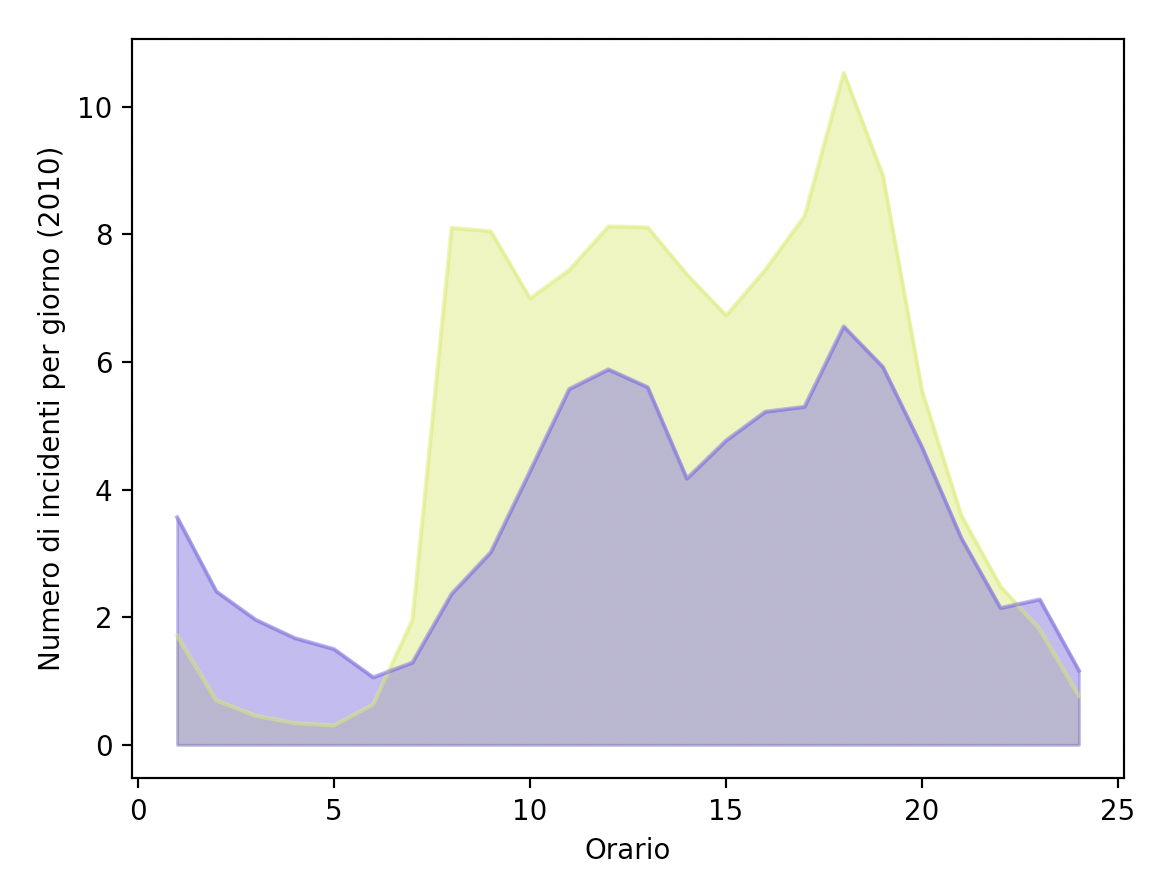
\includegraphics[width=\linewidth]{../src/incidenti/incidenti_senza_coords/ore_punta/week_weekend.png}
    \caption{Incidenti per ora}
    \label{fig:week-weekend}
\end{figure}

Tramite un semplice conto degli incidenti durante il weekend e, 
confrontando questo con il numero di quelli avvenuti durante la 
settimana lavorativa, si osserva che nel weekend avvengono più incidenti 
durante la sera e la notte, mentre durante la settimana in giornata.

Per quanto riguarda, invece, le fasce orarie 'di punta' definite precedentemente, 
sono state prese in considerazione, per la mattina, gli orari dalle 7:00 alle 10:00, 
e per il pomeriggio, dalle 17:00 alle 19:00.
L'incremento durante la fascia oraria pomeridiana è subito osservabile nella figura 
\ref{fig:week-weekend}, dove si ha un incremento del $95.2$\% di incidenti rispetto 
alla media durante la settimana lavorativa. 
D'altra parte, durante il weekend, si osserva comunque un incremento, ma solamente del $61.1$\%.

Per le fasce orarie della mattina, è comunque presente un incremento di incidenti, ma 
ammonta al $34.6$\% alle 8:00, e al $80.6$\% alle 9:00, mentre nel weekend si ha un 
decremento di incidenti in entrambi gli orari, rispettivamente del $47.6$\% e $17.9$\%.

\begin{lstlisting}[language=Python]
    ora_weekend = data[data['giorno'] > 5]['Ora'].value_counts().sort_index()
    ora_week = data[data['giorno'] < 6]['Ora'].value_counts().sort_index()

    ora_week /= 5 * 52
    ora_weekend /= 2 * 52
\end{lstlisting}

Va sottolineato che i grafi indicano gli incidenti normalizzati per numero di 
giorni, quindi gli incidenti totali della settimana sono divisi per cinque giorni, 
mentre quelli del weekend per due.

%\clearpage
\subsection{Incremento dell'incidentalità nelle fasce orarie della mattina}

I risultati della sezione precedente sembrano indicare che la maggior parte degli incidenti 
si verifica attorno alle 9:00 di mattina. Questa tendenza è vera anche nel caso in cui si 
isoli una città come Milano, dove arrivano molti pendolari dalla regione e che probabilmente sono 
già in viaggio prima delle 9:00?

Selezionano solo gli incidenti nella provincia di Milano, mostrati nel grafo 
\ref{fig:week-weekend-milano}, è possibile individuare in modo più preciso
il primo picco di incidenti, quello durante le ore di punta mattutine.
In particolare si ha un incremento del $34.3$\% alle 8:00 rispetto alla media, 
che cresce fino al $118.7$\% delle 9:00, nelle giornate lavorative;
d'altro canto, durante il weekend, il numero di incidenti cala del $58.5$\% rispetto alla media alle 8:00 
e del $37$\% alle 9:00.

\begin{figure}
    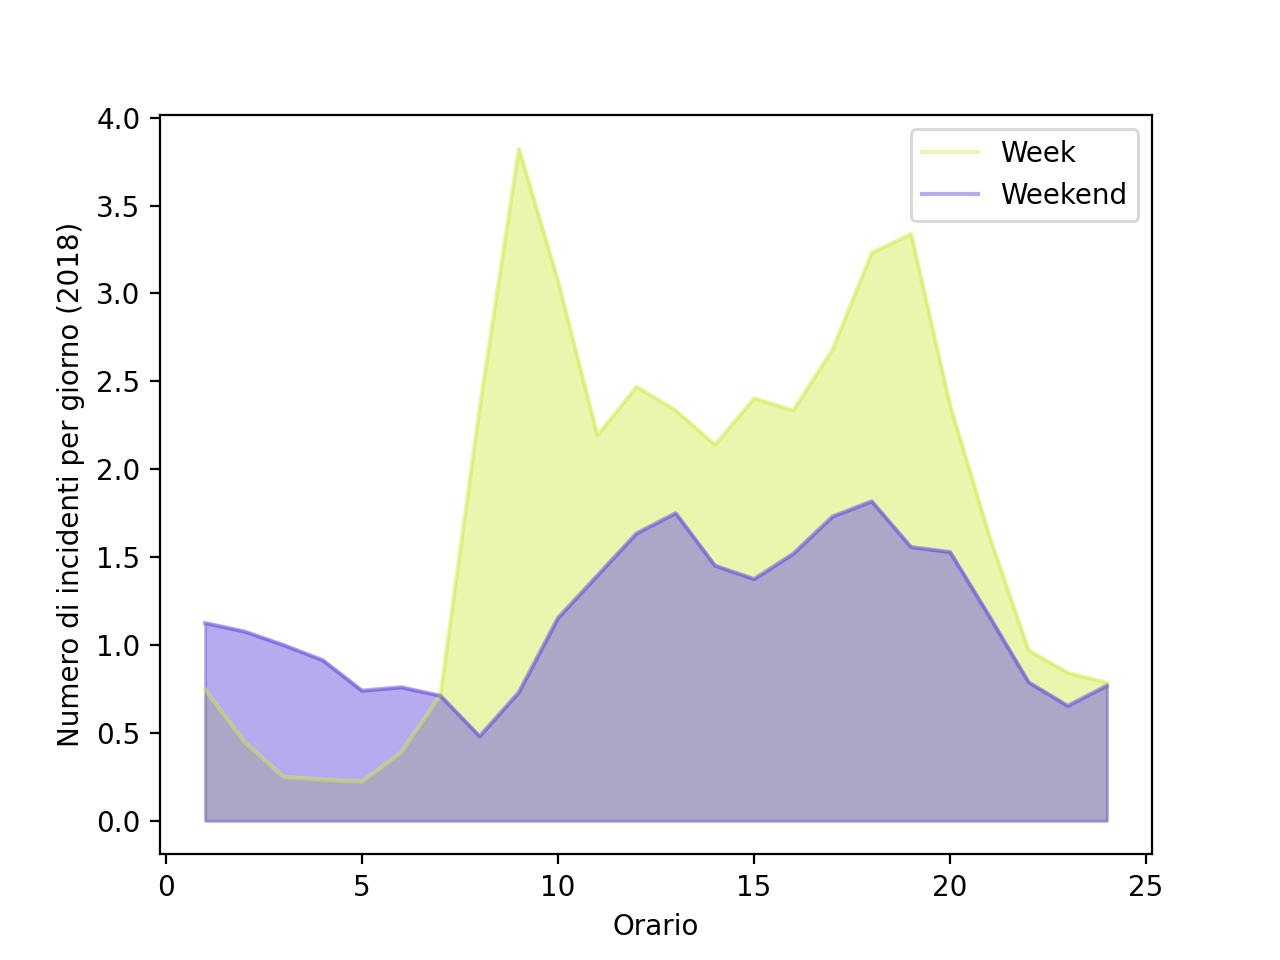
\includegraphics[width=\linewidth]{../src/incidenti/incidenti_senza_coords/ore_punta/week_weekend_milano.png}
    \caption{Incidenti per ora a Milano}
    \label{fig:week-weekend-milano}
\end{figure}

A Milano, dunque, si ha un incremento percentuale di incidenti alle 9:00 ancora maggiore,
rispetto al resto di Italia, e il flusso di pendolari, non sembra influenzare il volume di incidenti.

\subsection{Correlazione tra incidenti e traffico}

Fino a questo momento, si è parlato di incidenti senza alcun tipo di contesto, per quanto riguarda 
il numero di automobili presenti sulle strade. 
\'E chiaro che uno dei principali fattori alla causa degli incidenti sia il traffico, e sarebbe 
interessante riuscire a isolare l'impatto di quest'ultimo, nelle diverse ore della giornata.

Un primo problema da affrontare è quello di individuare informazioni sul traffico. 
Per quanto un dataset contenente questi dati non sia stato trovato, 
è possibile realizzare una stima di questo carattere a Milano, 
in quanto a partire dal 2011, fino al 2016, utilizzando i dati sul numero degli accessi all'area C.

\begin{figure}
    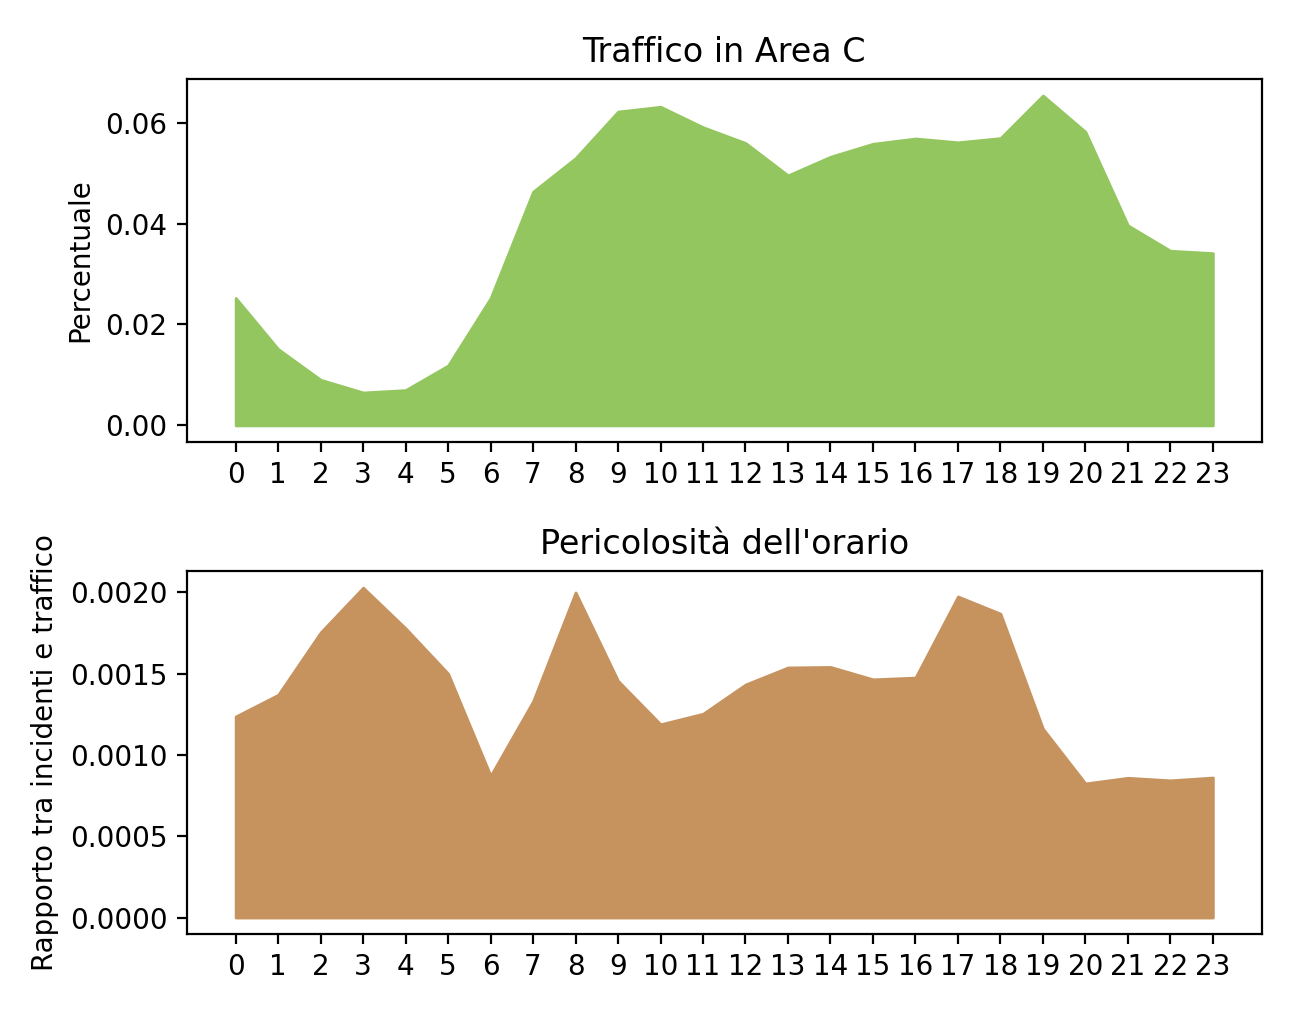
\includegraphics[width=\linewidth]{../src/area_c/rapporto_orario.png}
    \caption{Rapporto tra incidenti e traffico per orario a Milano}
    \label{fig:rapporto-incidenti-traffico}
\end{figure}

L'immagine \ref{fig:rapporto-incidenti-traffico} contiene, a partire dall'alto, 
la percentuale di accessi in area C a una determinata 
ora\footnote{Si sono utilizzati i dati dell'anno 2016, perchè non si sono trovati 
dataset più recenti per quanto riguarda gli accessi all'area C di Milano}, 
e il numero di incidenti a Milano, pesati in base al questa stima del traffico.

Si osservano molte similitudini tra la stima realizzata tramite gli ingressi 
in area C, rappresentata nel grafo sinistro della 
figura \ref{fig:rapporto-incidenti-traffico} e l'immagine \ref{fig:week-weekend-milano}, 
raffigurante gli incidenti a Milano divisi per orario, in particolare, 
la correlazione tra traffico in area C a Milano e numero incidenti per 
orario è $0.877$.

\begin{lstlisting}
    # eseguito con dati del 2016
    accessi_area_c_per_ora = pd.Series()
    for f in data['hour'].unique():
        accessi_area_c_per_ora = accessi_area_c_per_ora.append(
            pd.Series(data[data['hour'] == f]['totale'].sum()), 
            ignore_index=True
            )

    incidenti_per_ora = data[data['provincia'] == 15]['ora'].value_counts().sort_index()

    correlazione = accessi_area_c_per_ora.corr(incidenti_per_ora)
\end{lstlisting}

Per quanto riguarda invece, il grafo nella metà bassa della 
figura \ref{fig:rapporto-incidenti-traffico}, sono presenti tre picchi di 
con orari particolarmente pericolosi, uno alle 3:00 di mattina, uno alle 
8:00 e l'ultimo alle 18:00. 

Di questi, il primo è possibile che sia dovuto allo scarso volume di accessi 
all'area C in questo orario, visto che alle 3:00 di notte si ha il minimo volume di 
traffico della giornata, mentre gli altri due sono certamente dovuti all'alto 
numero di incidenti, in quanto il traffico in questi orari è pienamente nella media.

%\clearpage
\subsection{Incidentalità in orari notturni}

Nel grafo \ref{fig:week-weekend}, si è potuto osservare come, durante le 
ore notturne, si abbia il comportamento degli incidenti tra settimana lavorativa e weekend opposta.
Nella figura \ref{fig:ore-notte} sono raffigurate le principali ore della notte, divise tra 
settimana lavorativa e weekend.
Chiaramente, durante il weekend si hanno un maggior numero di incidenti negli orari serali e 
notturni, in particolare si hanno in media $5$ incidenti per serata in settimana, mentre il numero 
sale a $9.4$ durante il Sabato o la Domenica sera.

\begin{lstlisting}
    notte = data[(data['Ora'] < 7) | (data['Ora'] > 22)]
    ora_notte_week = notte[notte['giorno'] < 6]['Ora'].value_counts().sort_index()
    ora_notte_weekend = notte[notte['giorno'] > 5]['Ora'].value_counts().sort_index()

    ora_notte_week /= 5 * 52 
    ora_notte_weekend /= 2 * 52

    print(ora_notte_week.mean())
    print(ora_notte_weekend.mean())
\end{lstlisting}

Il traffico, stimato tramite gli accessi all'area C, conferma la tendenza?

\begin{figure}
    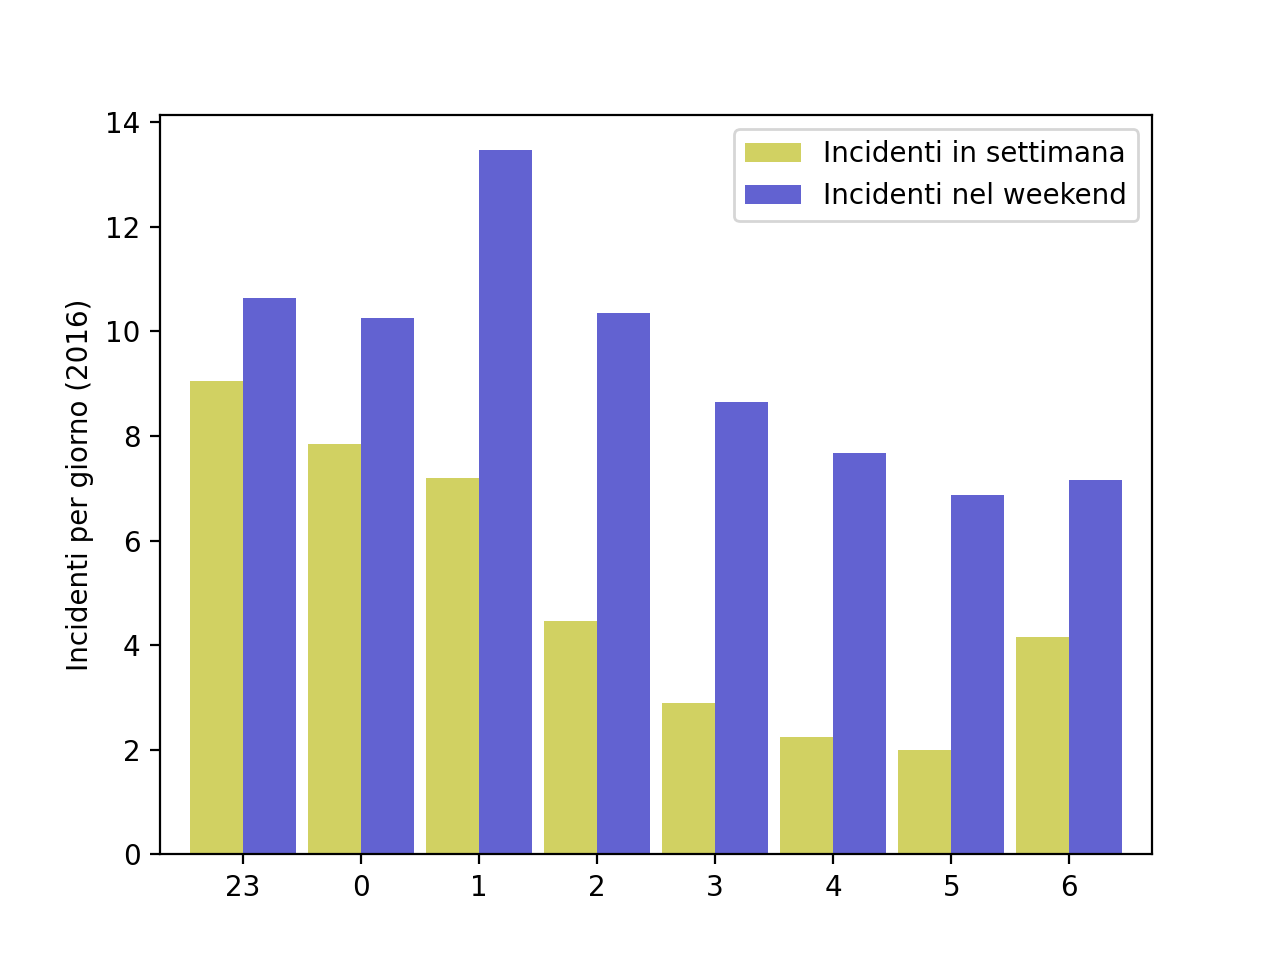
\includegraphics[width=0.5\linewidth]{../src/incidenti/incidenti_senza_coords/ore_punta/ore_notte.png}
    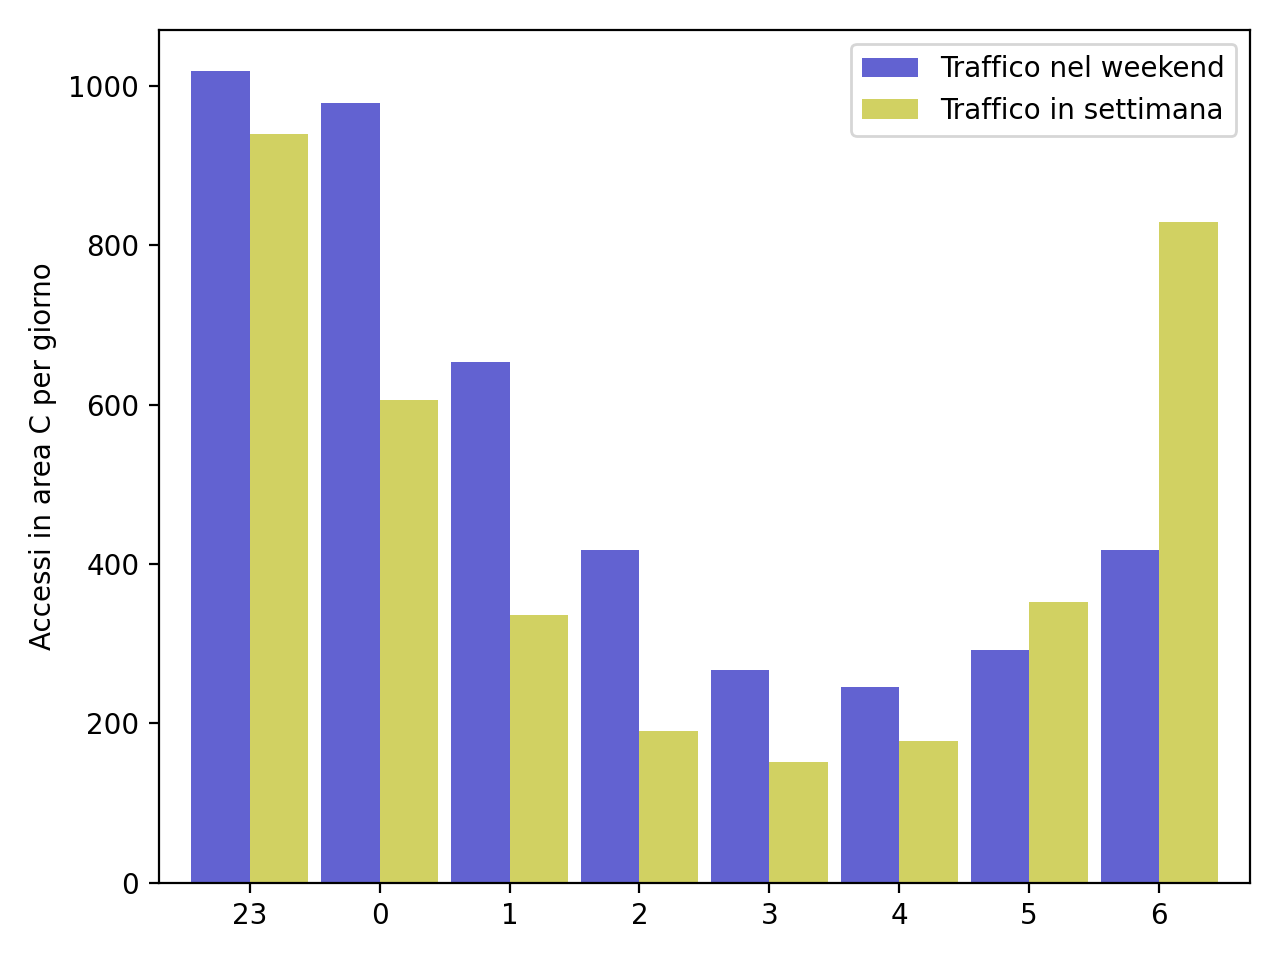
\includegraphics[width=0.48\linewidth]{../src/area_c/traffico_serale.png}
    \caption{Incidenti e traffico durante ore serali o notturne}
    \label{fig:ore-notte}
\end{figure}

Va detto che la differenza di traffico tra settimana lavorativa e weekend in orari serali non è molta, 
e che il divario maggiore è presente alle ore 6:00 in favore del traffico in settimana.
D'altra parte il traffico nel weekend è maggiore in quasi tutte le altre ore.

Una volta ottenuti questi risultati,  è possibile calcolare quali sono le ore più pericolose, 
eseguendo il rapporto tra incidenti e traffico per orario.
Il risultato del calcolo è rafficurato nel grafo \ref{fig:rapp-inc-traff}.

\begin{figure}
    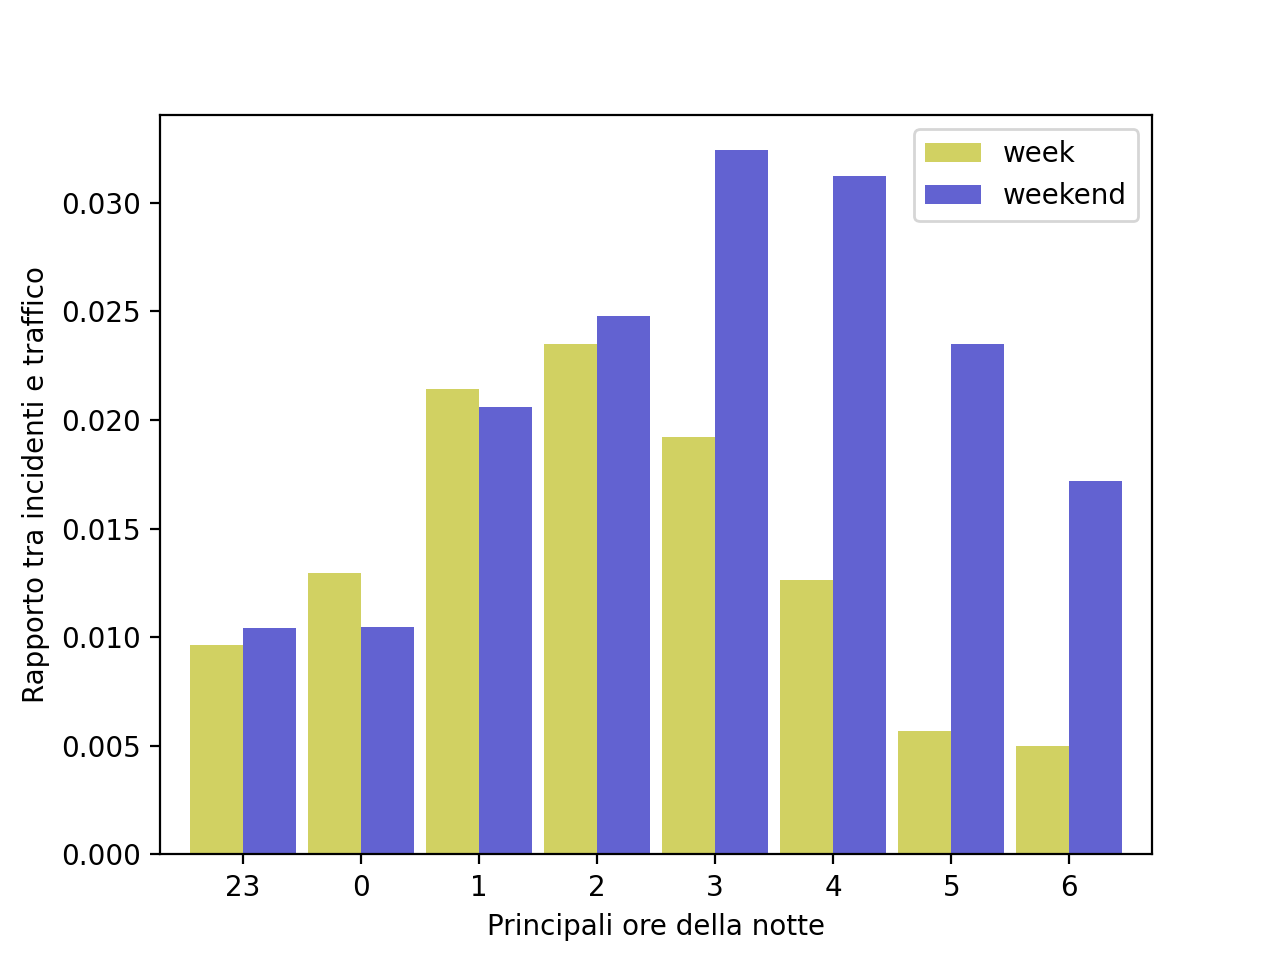
\includegraphics[width=\linewidth]{../src/area_c/rapporto_inc_notte.png}
    \caption{Rapporto tra incidenti e traffico durante ore serali o notturne}
    \label{fig:rapp-inc-traff}
\end{figure}

Per quanto riguarda il weekend, le ore più pericolose sono tra le 3:00 e le 4:00 di notte, mentre per 
la settimana lavorativa le ore più pericolose sono quelle tra 1:00 e 3:00, e il numero di 
incidenti rapportato al traffico è anche molto minore. 

I risultati sembrano essere in linea con l'idea che, nel weekend il maggior 
numero di incidenti avviene in ore più tarde a causa della movida, mentre nella settimana lavorativa 
meno persone sono sveglie nelle ore notturne.

%\clearpage
\subsection{Quanto influiscono le vacanze estive sull'incidentalità?}

Sarebbe interessante individuare eventuali cali o incrementi di incidenti, per quanto riguarda gli 
incidenti su intervallo mensile.
Il dataset sugli accessi all'area C è presente, nel caso della divisione per mese, fino all'anno 2018, 
tuttavia i dati istat su incidenti contengono il campo \columnstyle{mese} solo fino all'anno 2013,
dunque i grafi sull'argomento prenderanno in considerazione quest'annata più recente.

\begin{figure}
    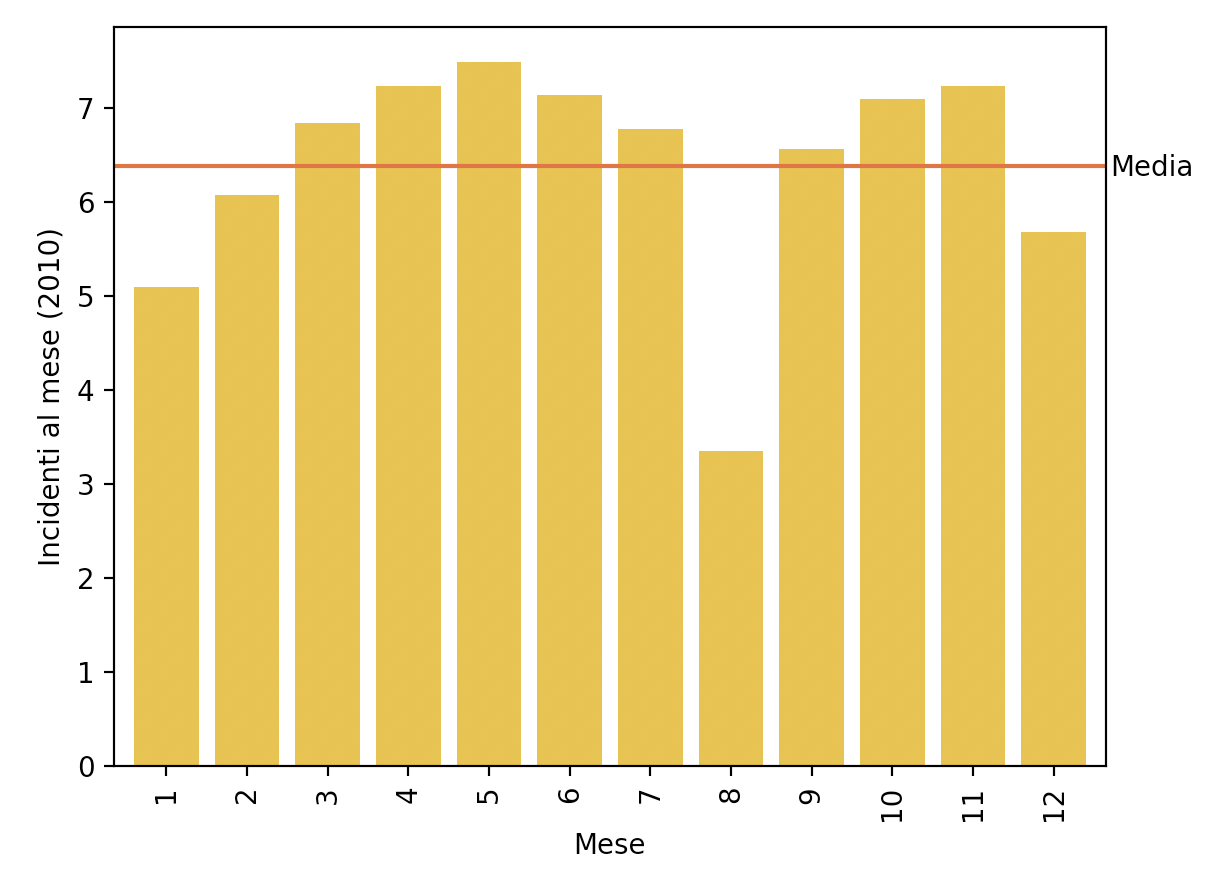
\includegraphics[width=\linewidth]{../src/incidenti/incidenti_senza_coords/mese_incidenti/milano_mese.png}
    \caption{Incidenti per mese in Milano}
    \label{fig:milano-mese}
\end{figure}

Nel grafo \ref{fig:milano-mese} si nota un chiaro calo di incidenti nel mese di 
Agosto in provincia di Milano, la percentuale di decremento è riportata nella tabella sottostante, 
anche per gli altri anni per cui sono disponibili i dati.


\begin{center}
    \def\arraystretch{1.5}%  
    \begin{tabular}{ |c|c| } 
        \hline
        Anno & Decremento in Agosto \\ 
        \hline
        2010 & 47.4\%  \\ 
        \rowcolor{TableGray}
        2011 & 35.14\% \\
        2012 & 45.46\% \\
        \rowcolor{TableGray}
        2013 & 41.37 \% \\
        \hline
    \end{tabular}
\end{center}

Per quanto possano esserci molti fattori che contribuiscono a questa tendenza di decremento di sinistri, 
quello che influisce di più devono essere le partenze per le vacanze estive.

Un modo per testare questa teoria è controllare se il traffico durante il mese di Agosto cala a 
Milano, stimato tramite i dati sugli accessi in area C. 
A supporto dell'ipotesi iniziale, nella figura \ref{fig:stima-traffico-mensile}, 
è visibile un calo di accessi all'area C durante il mese di Agosto.

\begin{figure}
    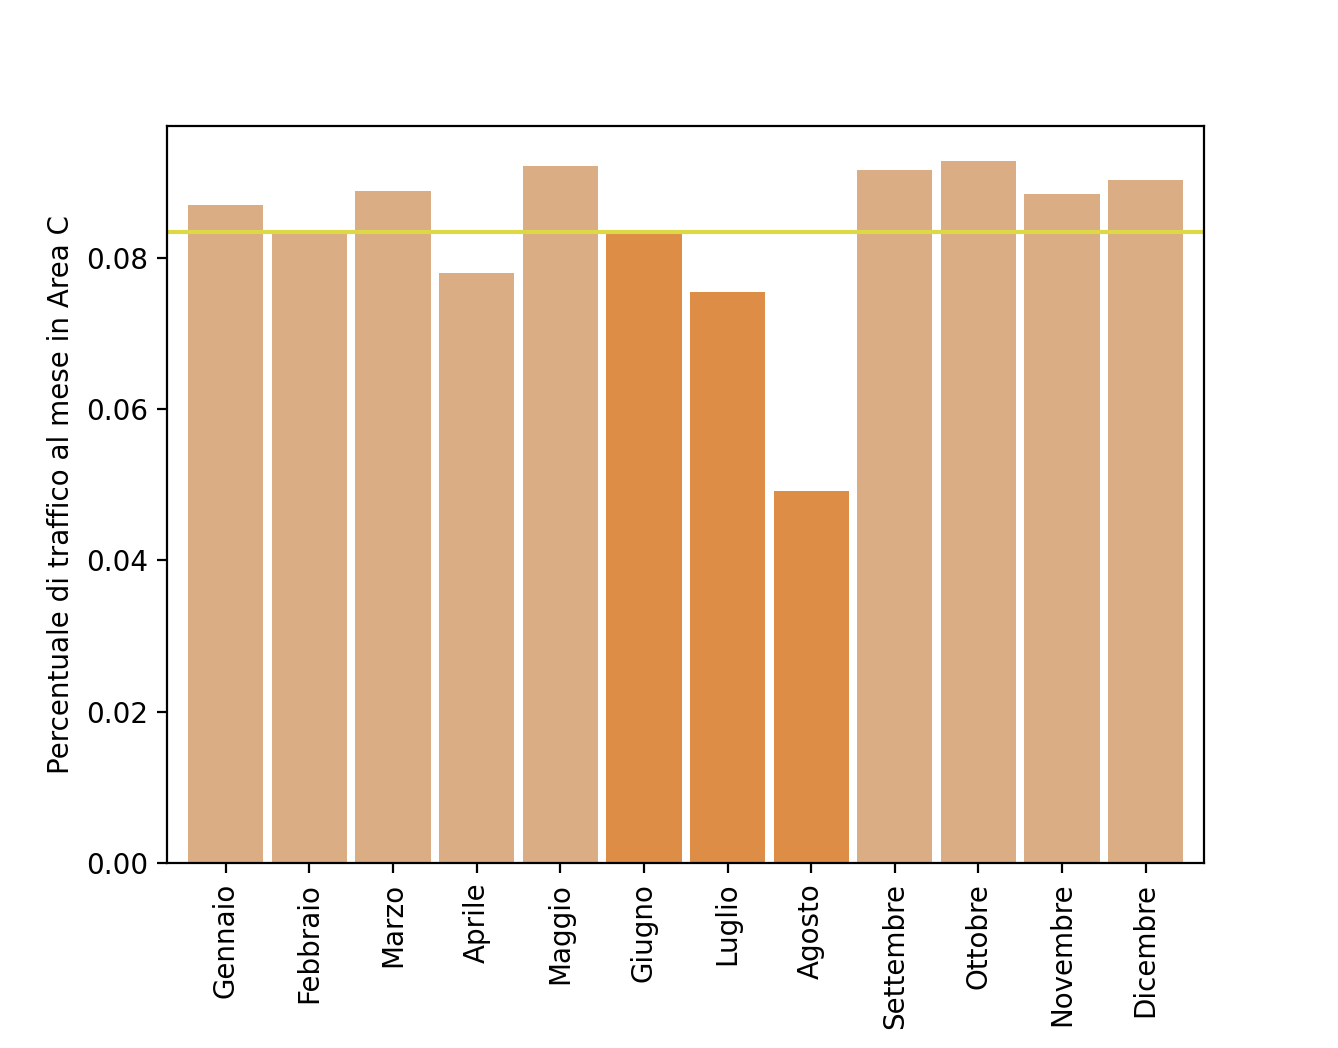
\includegraphics[width=\linewidth]{../src/area_c/stima_traffico_mese.png}
    \caption{Stima del traffico a Milano per mese, tramite accessi all'area C}
    \label{fig:stima-traffico-mensile}
\end{figure}

Una volta ottenuta una stima del traffico per mese, è possibile applicare questa misurazione 
al numero di incidenti mensili.

\begin{figure}
    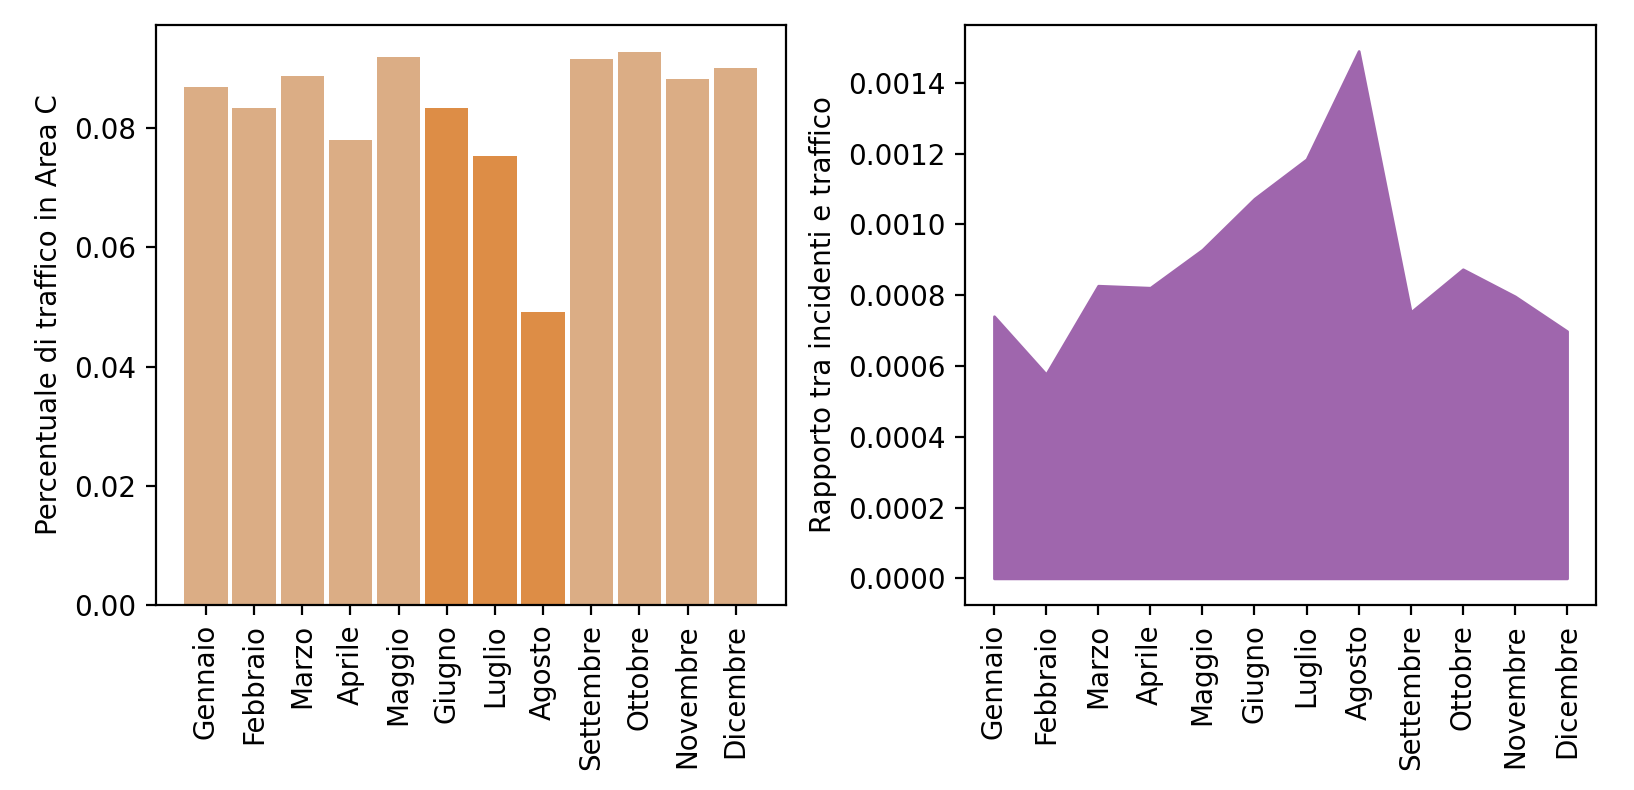
\includegraphics[width=\linewidth]{../src/area_c/rapporto_mese.png}
    \caption{Incidenti al mese, tenendo conto del traffico nello stesso periodo (2012)}
    \label{fig:incidenti-traffico-mese}
\end{figure}

L'immagine \ref{fig:incidenti-traffico-mese} contiene due grafi, 
il primo riguardante la frazione di traffico annuale che interessa ogni mese; 
mentre il secondo raffigura il rapporto tra il numero di incidenti mensili, e il traffico 
stimato mensile\footnote{Si è utilizzato l'anno 2012 perchè è il primo anno contenente tutti i dati completi, 
tutti gli altri anni hanno mesi o campi mancanti}.
Nel secondo grafo della figura \ref{fig:incidenti-traffico-mese}, si osserva come, per quanto agosto 
abbia il minor numero di incidenti mensili, una volta tenuto conto della minore quantità di traffico, 
risulta essere il mese più pericoloso.

A partire dal 2014, il campo \columnstyle{mese} è stato convertito nella 
colonna \columnstyle{trimestre}.
La figura \ref{fig:milano-trimestri} mostra la quantità di incidenti per trimestre per ogni 
anno a partire dal 2010 fino al 2018.

\begin{figure}
    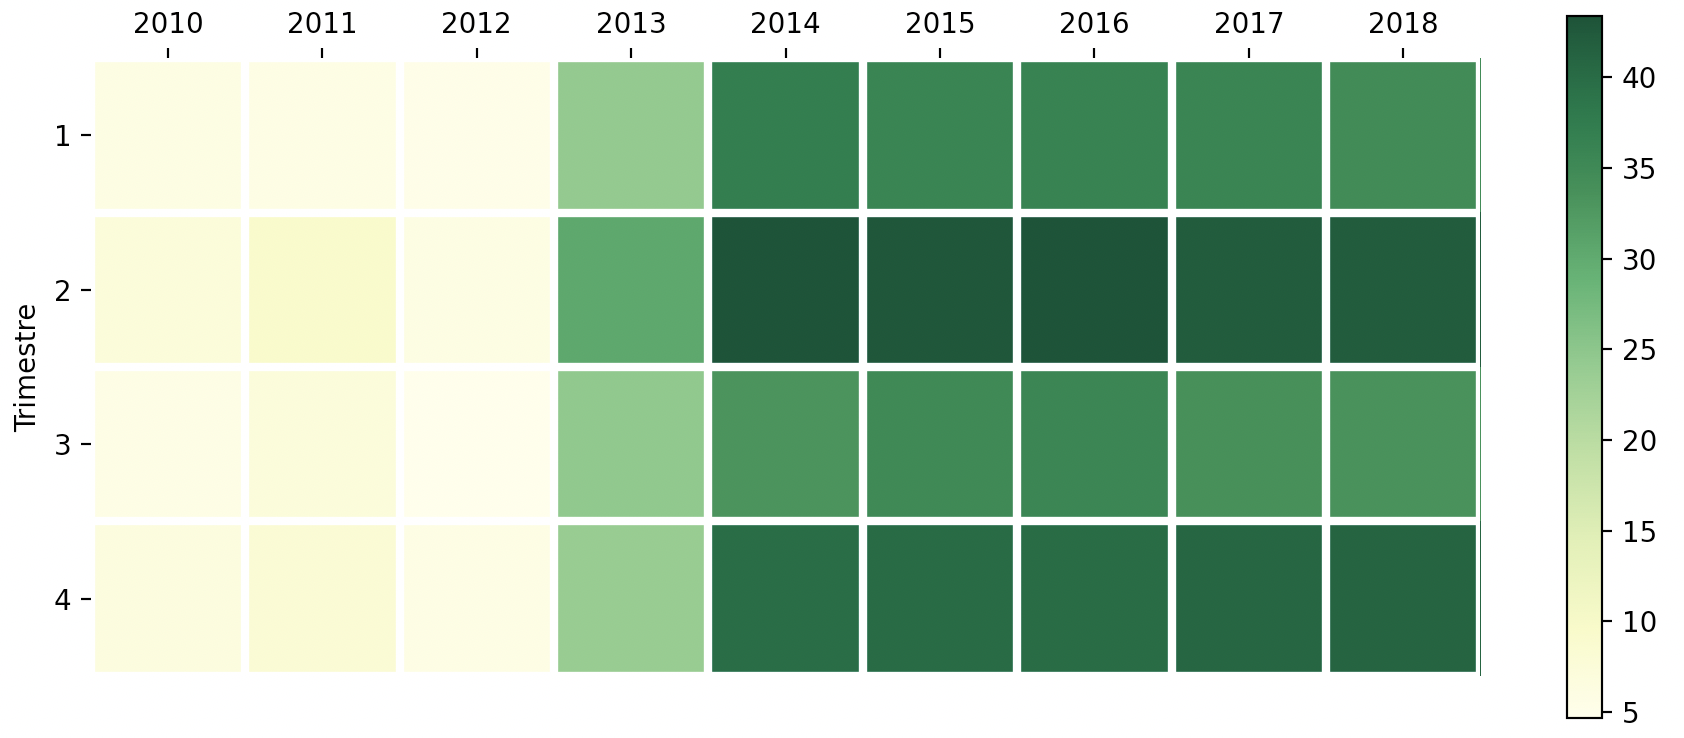
\includegraphics[width=\linewidth]{../src/incidenti/incidenti_senza_coords/mese_incidenti/trimestri.png}
    \caption{Incidenti a Milano per trimestre}
    \label{fig:milano-trimestri}
\end{figure}

Anche nel caso dei trimestri, quello estivo ha un numero minore di incidenti, ma il volume è 
comparabile con quello del primo trimestre, mentre durante il secondo e il quarto avvengono 
decisamente più incidenti.


%\clearpage
\subsection{In località di mare gli incidenti aumentano in estate?}

La domanda che sorge spontanea, una volta visto il grafo in figura \ref{fig:milano-mese}, è se 
il numero basso di incidenti in Agosto corrisponda con un numero alto di sinostri in altre località 
di vacanza. 

Nalla figura \ref{fig:mesi-estivi} sono elencate le province con maggiore incidentalità 
in Agosto rispetto a tutto l'anno. In particolare, ad aumentare in volume sono le 
province di Brescia e Palermo.

\begin{figure}
    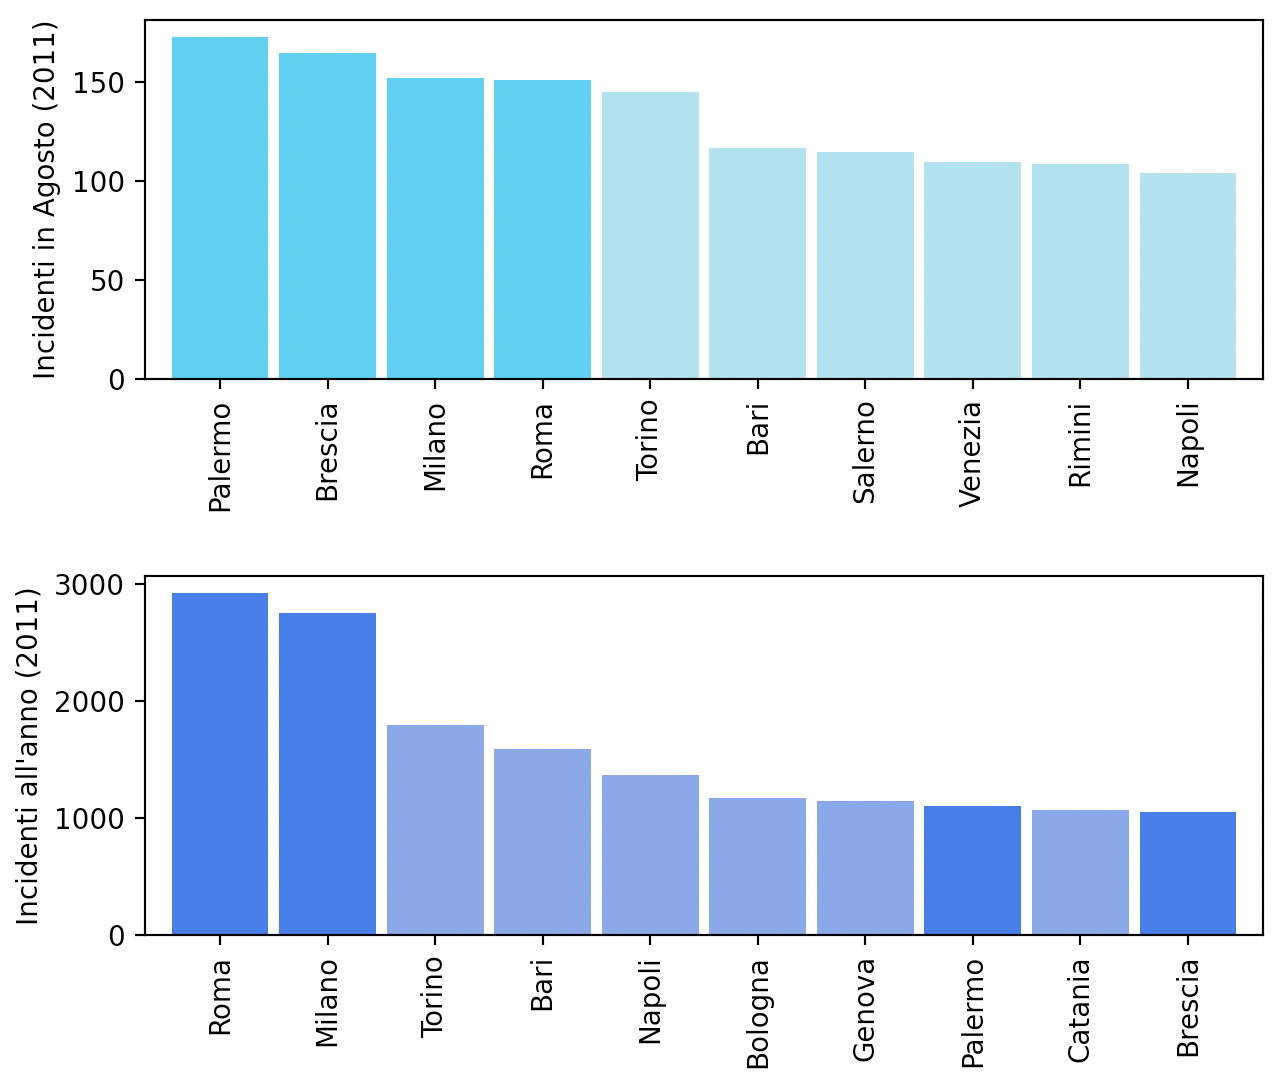
\includegraphics[width=\linewidth]{../src/incidenti/incidenti_senza_coords/mese_incidenti/mesi_estivi.png}
    \caption{Prime 10 province per incidenti in Agosto rispetto a tutto l'anno}
    \label{fig:mesi-estivi}
\end{figure}

Tuttavia questo comportamento è unico dell'anno 2011, in quanto, per gli altri due anni in cui 
si dispone dei dati sui mesi, 2012 e 2013, Milano e Roma hanno il primato di 
incidenti sia per l'anno che per il mese di Agosto individuale.

Ipotizzando invece, di comparare più nel dettaglio alcune province, meta di vacanze estive, 
con Milano, ciò che ci si aspetta da queste ultime è di avere un incremento di incidenti nei mesi 
di Luglio e Agosto\footnote{Si è utilizzato l'anno più recente per i dati a disposizione, 
a partire dal 2014 non sono più disponibili dati riguardanti il mese}.

Per eseguire questo confronto sono state prese in considerazione le località di Rimine e Palermo, 
per mostrare che alcune province, come la prima, confermano l'ipotesi, mentre altre, come la seconda, 
sembrano andare contro.

\begin{figure}
    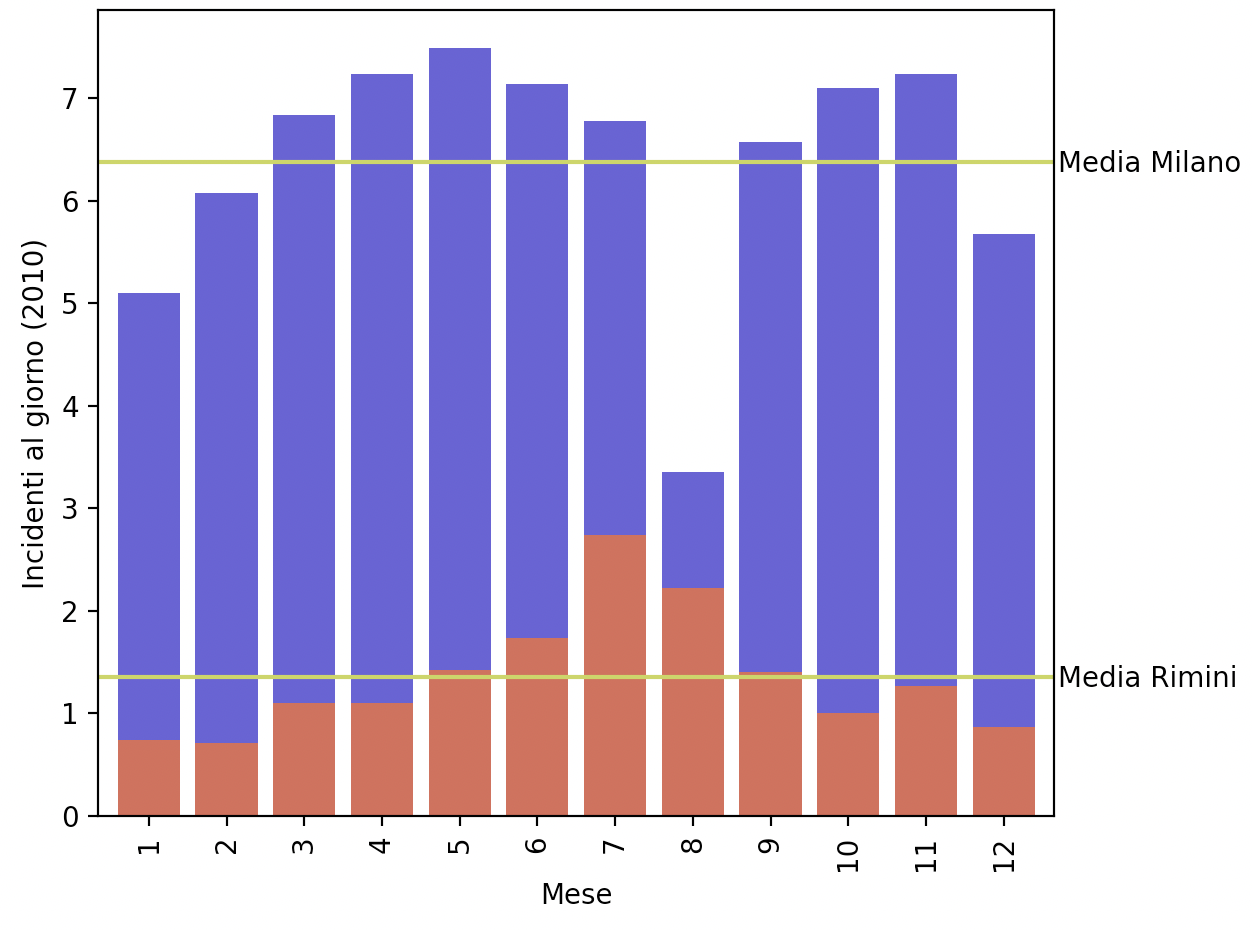
\includegraphics[width=\linewidth]{../src/incidenti/incidenti_senza_coords/mese_incidenti/milano_rimini.png}
    \caption{Incidenti per mese a Milano e Rimini}
    \label{fig:milano-rimini}
\end{figure}

\begin{figure}
    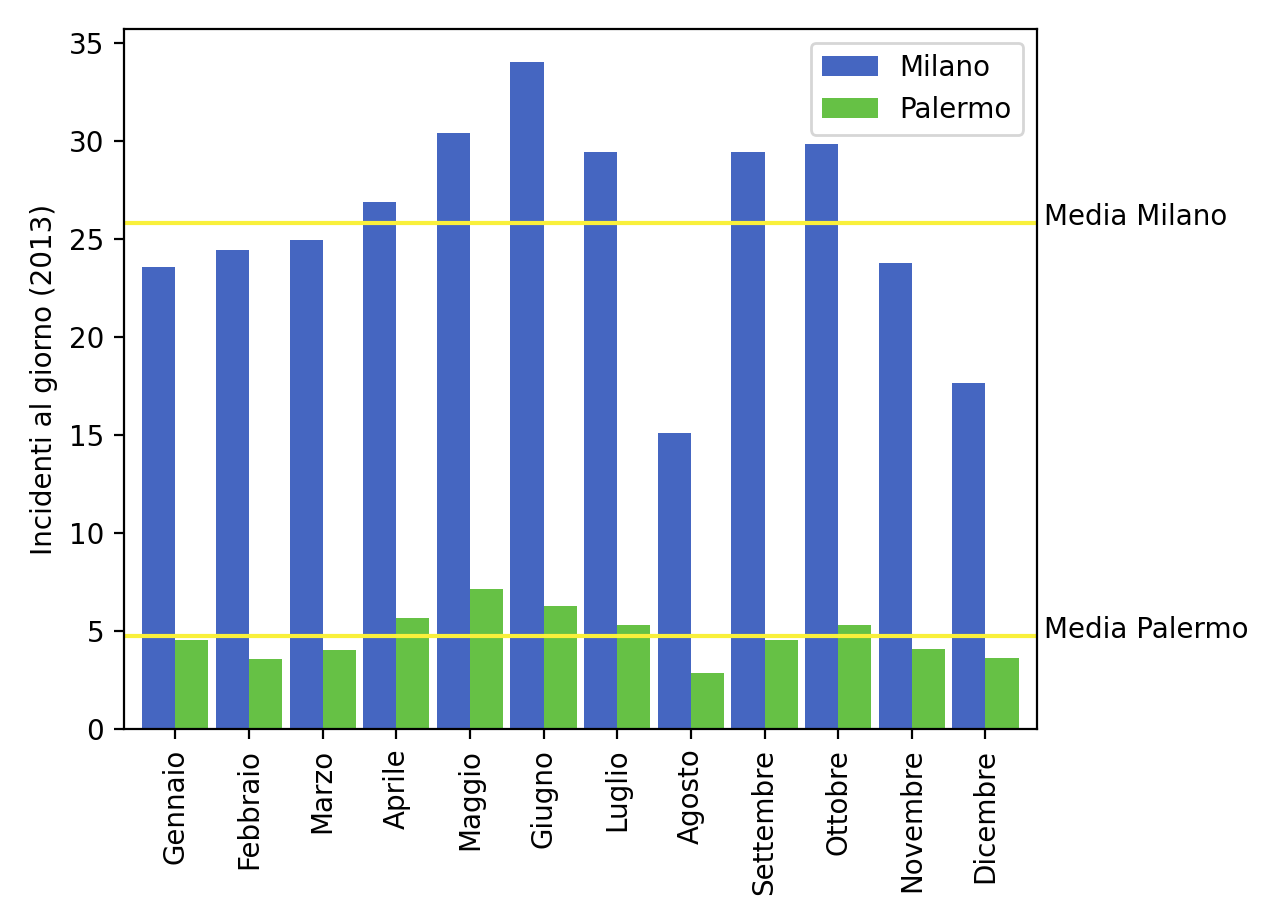
\includegraphics[width=\linewidth]{../src/incidenti/incidenti_senza_coords/mese_incidenti/palermo_milano.png}
    \caption{Incidenti per mese a Milano e Palermo}
    \label{fig:palermo-milano}
\end{figure}

Il confronto tra Milano e Rimini è raffigurato nell'immagine \ref{fig:milano-rimini} e, per quanto a 
Milano avvengano un numero molto maggiore di incidenti rispetto alla provincia Emiliana, nei mesi estivi, 
il numero di sinistri a Rimini è superiore alla media annuale, mentre per Milano è inferiore.

Nella provincia di Palermo, visibile in figura \ref{fig:palermo-milano}, d'altra parte, 
non risulta che nessun mese abbbia un numero di incidenti 
particolarmente più alto della media.

Nella seguente tabella, sono indicati gli incrementi per anno del numero di incidenti a Rimini.
L'incremento constante per ogni anno, conferma che questo fenomeno è un trend annuale.

\begin{center}
    \def\arraystretch{1.5}%  
    \begin{tabular}{ |c|c|c| } 
    \hline
    Anno & Luglio   & Agosto \\ 
    \hline
    \rowcolor{TableGray}
    2010 & 101.72\% & 63.75 \% \\ 
    2011 & 54.6  \%  & 60.49\% \\
    \rowcolor{TableGray}
    2012 & 75.97 \%  & 45.93\%\\
    2013 & 116.37\% & 51.82 \%\\
    \hline
    \end{tabular}
\end{center}

Osservando il grafo raffigurante gli incidenti per mese della Valle d'Aosta, in figura \ref{fig:aosta}, 
è possibile notare un notevole incremento di incidenti sia in Gennaio che in Agosto, possibili 
conseguenze, rispettivamente, dell'inizio della stagione sciistica ed estiva.

\begin{figure}
    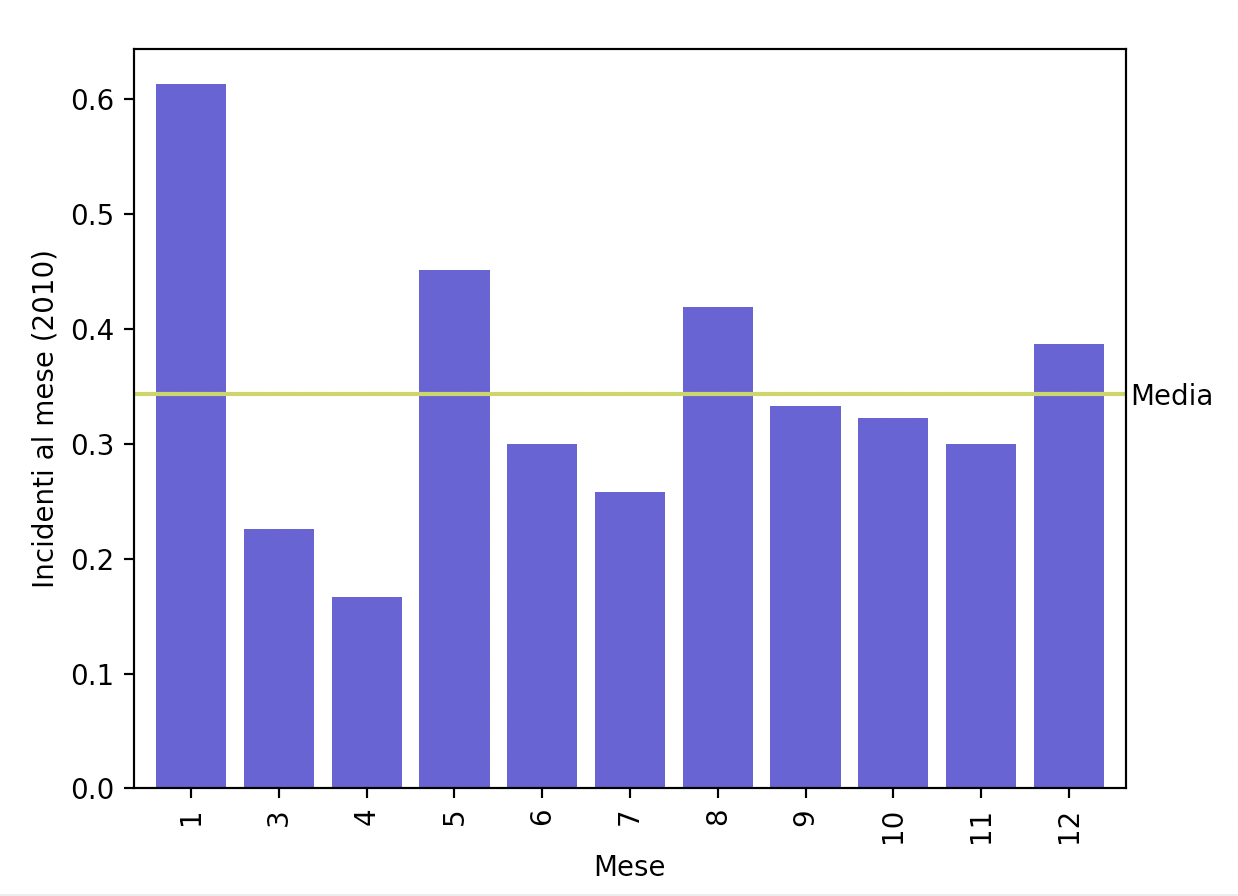
\includegraphics[width=\linewidth]{../src/incidenti/incidenti_senza_coords/mese_incidenti/aosta_mese.png}
    \caption{Incidenti per mese Valle d'Aosta}
    \label{fig:aosta}
\end{figure}

Questa tendenza avviene ogni anno?

\begin{center}
    \def\arraystretch{1.5}%  
    \begin{tabular}{ |c|c|c| } 
    \hline
    Anno & Gennaio & Agosto \\ 
    \hline
    \rowcolor{TableGray}
    2010 & 78.48\%  & -2.93 \%\\ 
    2011 & -32.12\% & 124.0 \%\\
    \rowcolor{TableGray}
    2012 & -41.44\% & 52.25 \% \\
    2013 & -24.63\% & -15.21\% \\
    \hline
    \end{tabular}
\end{center}

Il comportamento degli incidenti in Valle d'Aosta, mostrato in figura 
\ref{fig:aosta-rimini-milano-trimestre} è molto inconsistente, soprattutto in Agosto.
Va specificato che la taglia del campione con cui si sta lavorando, per questa provincia, 
è molto piccolo, e sicuramente influisce sulle percentuali di incremento e decremento 
degli incidenti.\\
Nonostane ciò, se si assume che Gennaio 2010 sia un outlier, il numero di incidenti in 
questo mese è sempre in decremento, in modo molto consistente, rispetto alla media.

Per avere una visione di insieme delle tendenze annuali, è possibile tracciare 
un grafo contenente gli incidenti divisi per trimestre dove, per esempio, 
per primo trimestre si intende Gennaio, Febbraio e Marzo.

\begin{figure}
    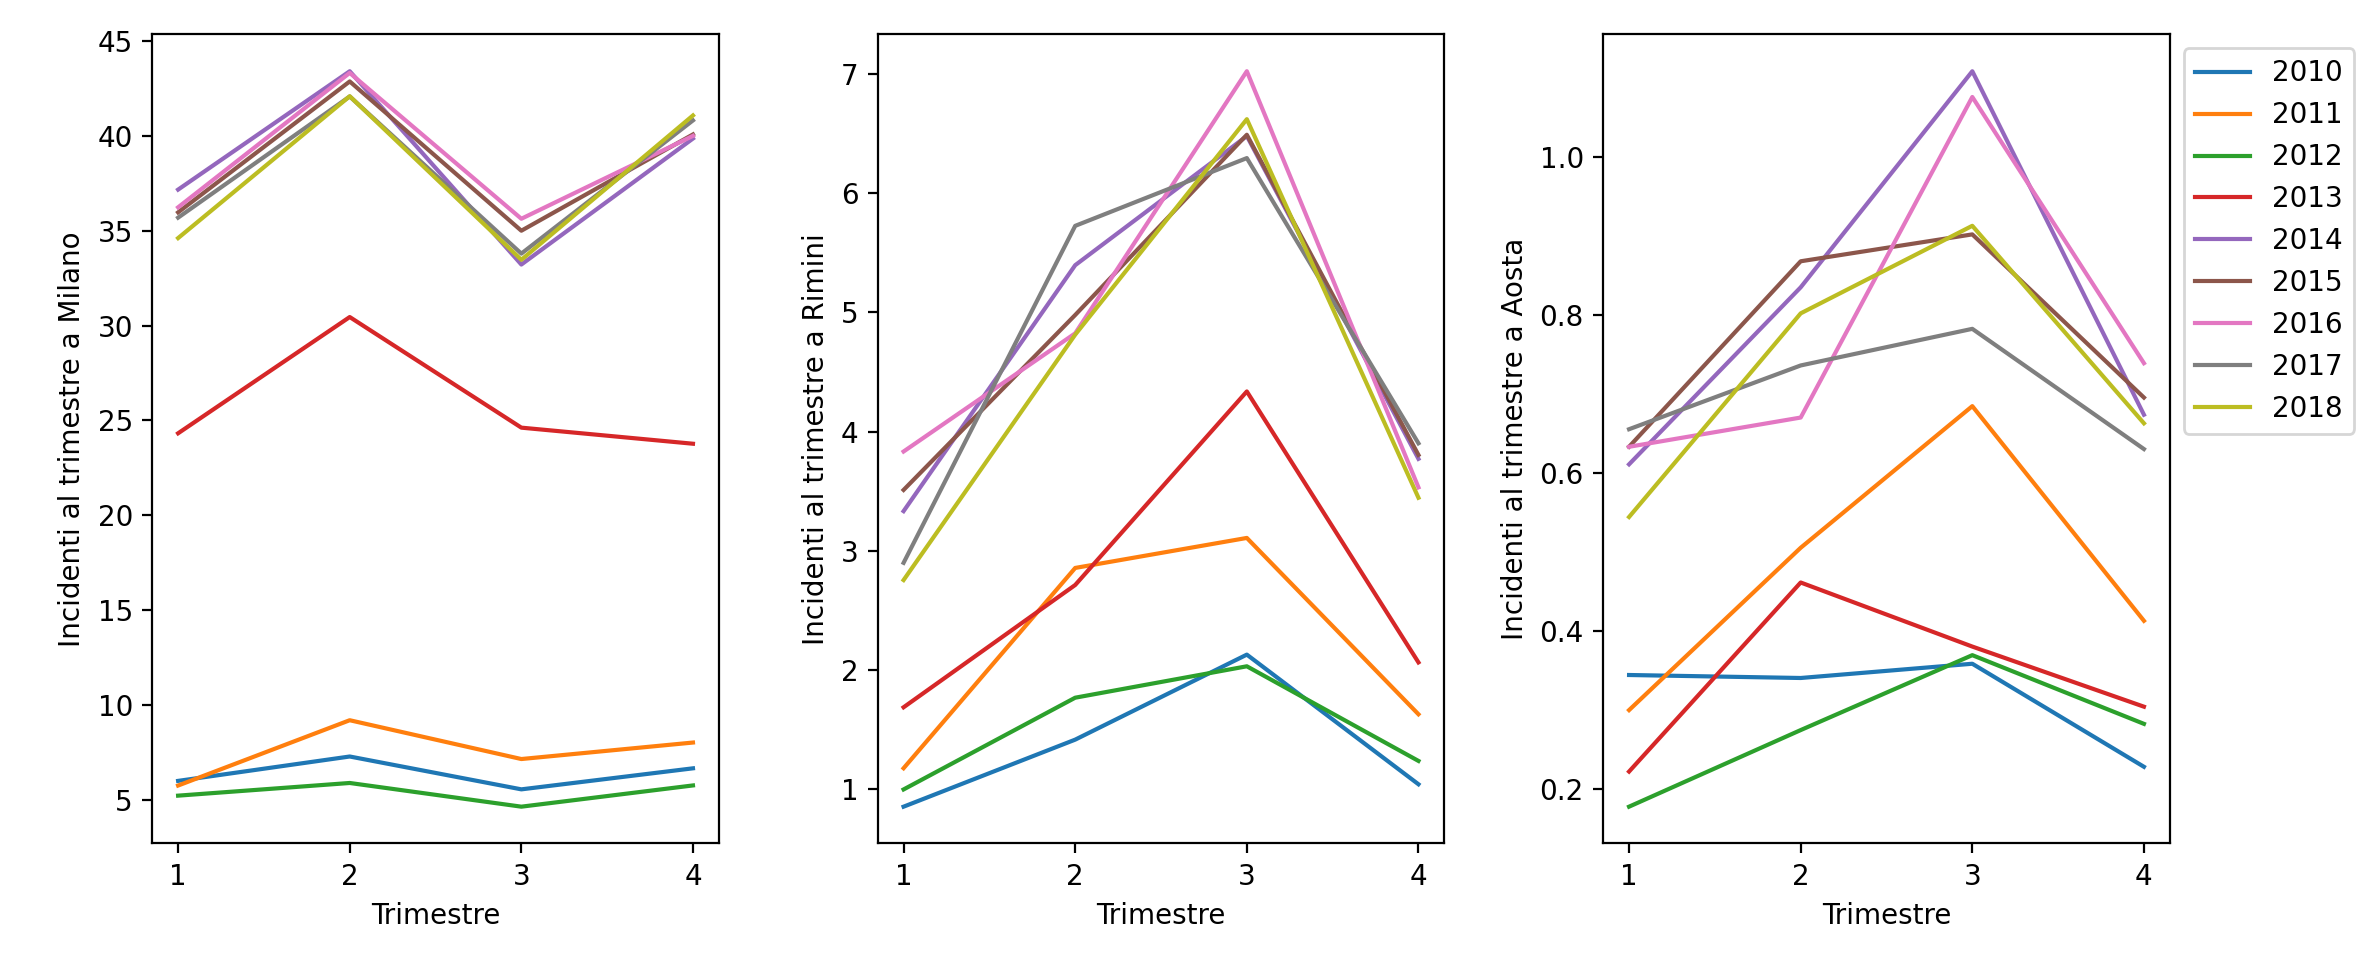
\includegraphics[width=\linewidth]{../src/incidenti/incidenti_senza_coords/mese_incidenti/trimestri_aosta_milano_rimini.png}
    \caption{Incidenti per trimestre in Valle d'Aosta, a Rimini e a Milano}
    \label{fig:aosta-rimini-milano-trimestre}
\end{figure}

In tutti i grafi nella figura \ref{fig:aosta-rimini-milano-trimestre}, 
si osserva di nuovo, dall'anno 2015, l'ampio gap nel numero di incidenti, 
probabilmente dovuto a un cambio di misurazione degli incidenti, di cui si 
è parlato in un precedente capitolo. 

Per quanto riguarda Rimini e Aosta, si osservano varie similitudini, con quasi 
tutte le annate, in particolare si osserva un basso numero di incidenti 
durante il primo trimestre, e un incremento di sinistri durante il terzo trimestre.

D'altra parte, a Milano, si ha la tendenza opposta, con maggior numero di 
incidenti nel secondo trimestre, e un abbassamento durante il primo 
e terzo trimestre.

Ciò che è possibile dedurre, è che a Milano il numero di incidenti decresce 
nel terzo trimestre in accordo con le partenze per le vacanze, mentre nelle 
altre località raffigurate, avviene la tendenza opposta poichè 
queste sono mete feriali.

Sarebbe interessante conoscere se esistono località di vacanza preferite, o se 
queste cambiano il base all'anno, si tenterà di rispondere a queste domande 
nei capitoli successivi.

%\clearpage
\section{Dati Istat su tipi di incidenti e incroci}

A riguardo dei dati sulla località degli incidenti e del tipo di incrocio, 
sarebbe interessante sapere se esistano tipologie di incidenti che accadono 
con più frequenza di altre, o se tra queste tipologie, il numero di feriti 
è comparabile o se alcuni incidenti sono più pericolosi di altri.

%\clearpage
\subsection{Le tipologie di incidenti più frequenti}

\begin{figure}
    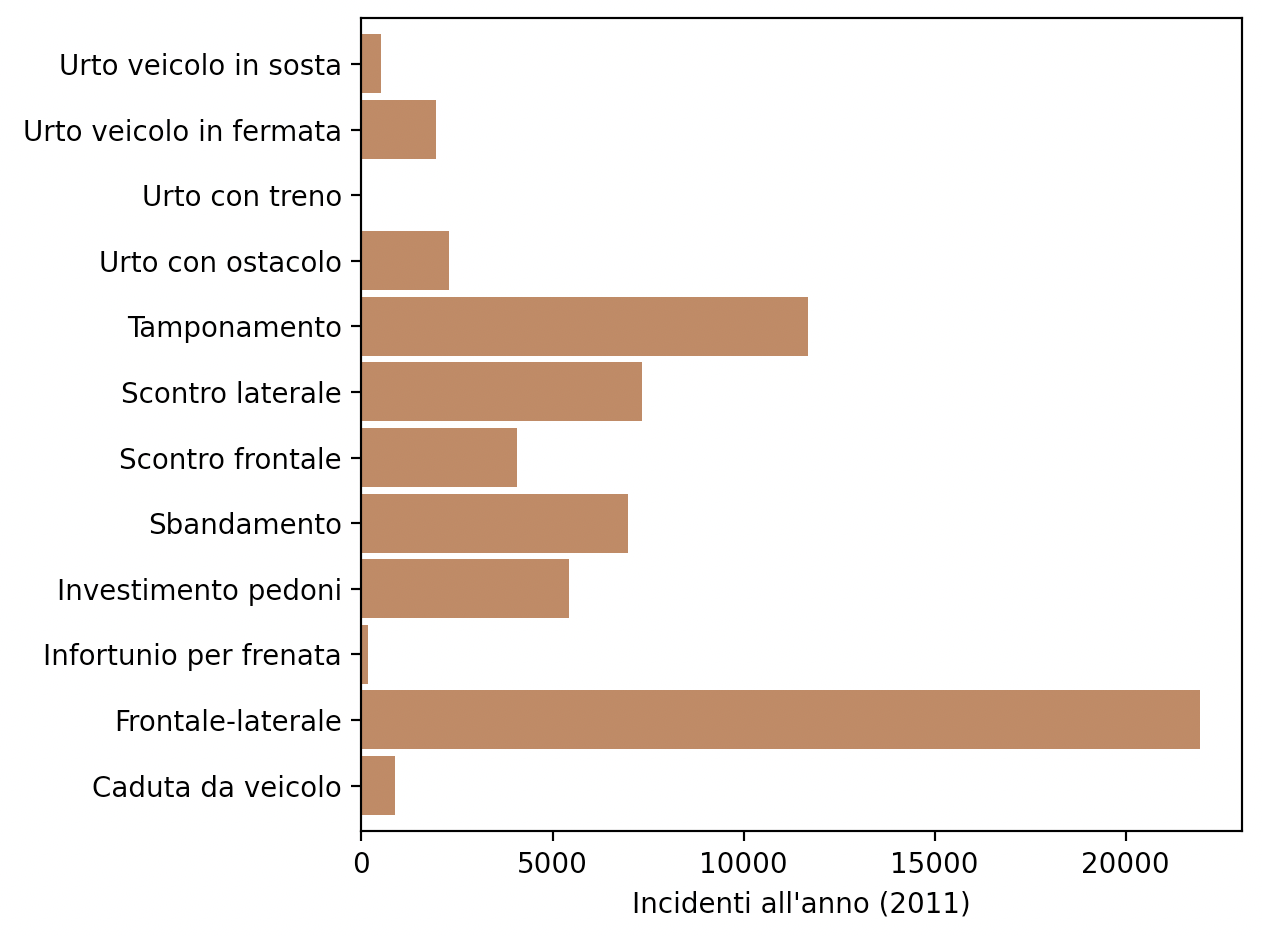
\includegraphics[width=\linewidth]{../src/incidenti/incidenti_senza_coords/localizzazione_incidente/tipo_incidente.png}
    \caption{Tipologia di incidente}
    \label{fig:tipo-incidente}
\end{figure}

Nella figura \ref{fig:tipo-incidente} è possibile osservare quali sono gli incidenti 
più frequenti in un anno, in questo caso nel 2018.
In particolare sono molto frequenti scontri frontali, laterali e tamponamenti. 
Gli incidenti frontali-laterali sono i più rappresentati probabilmente per 
l'ampiezza della categoria.

Questo grafo, senza un constesto, non è molto utile. Tuttavia è difficile 
individuare un fattore che incida particolarmente sulle diverse tipologie di incidente.

Ciò che è possibile controllare, è se negli altri anni disponibili, il rapporto 
di tipologie di incidenti rimanga costante o no.
Le percentuali delle prime quattro categorie di incidenti sono riportate nella 
figura \ref{fig:rapporto-tipologie}: 

\begin{figure}
    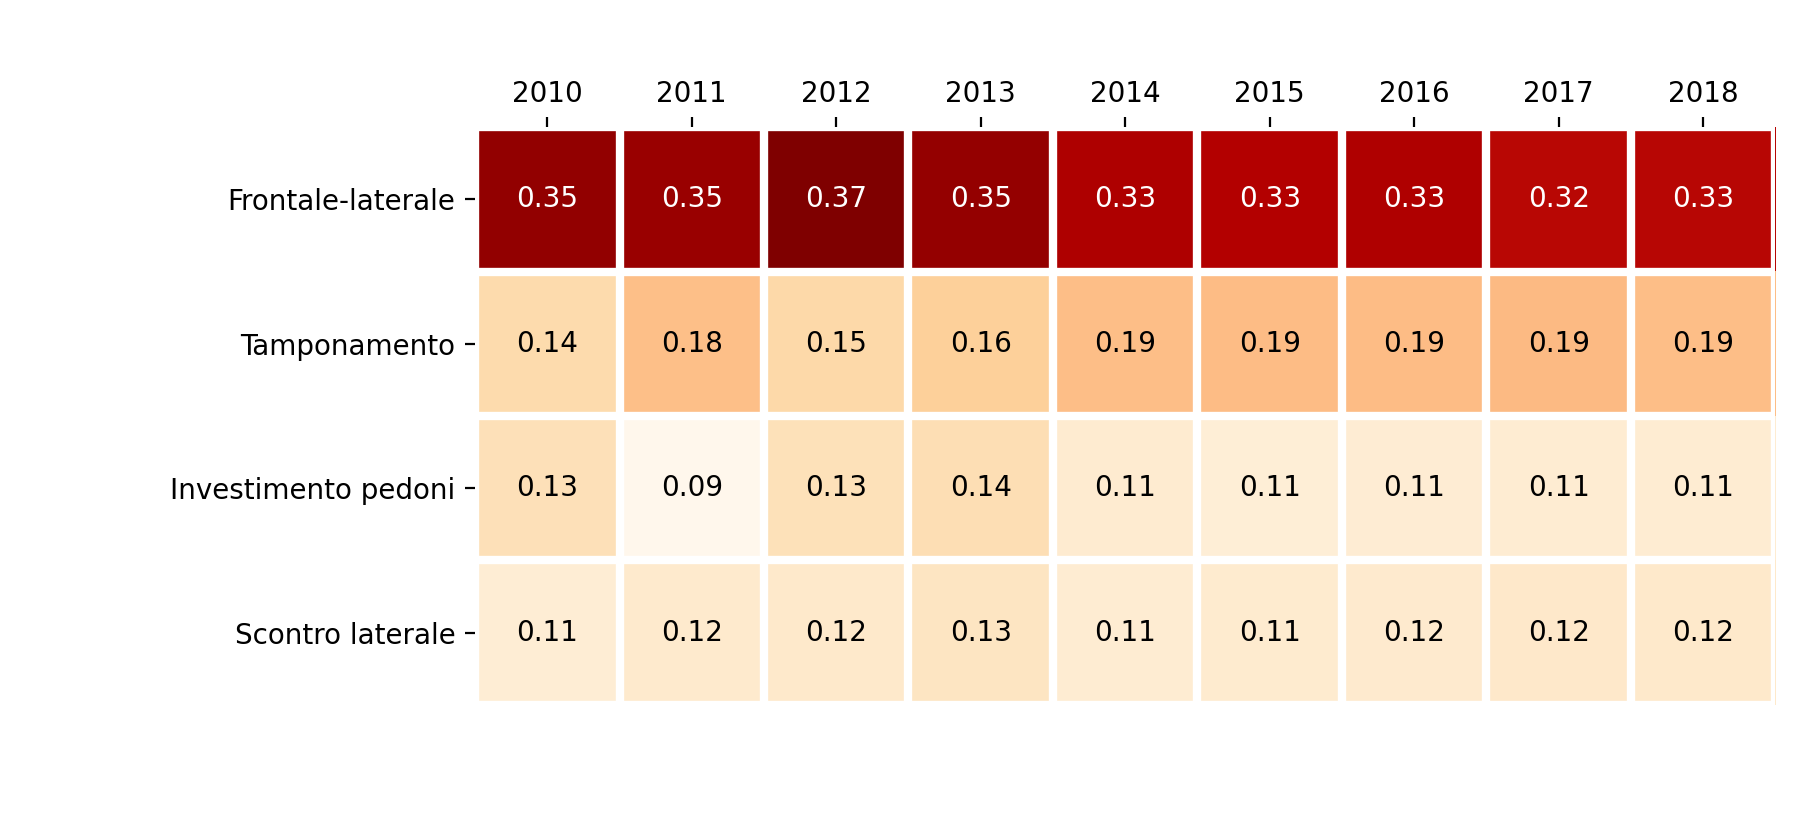
\includegraphics[width=\linewidth]{../src/incidenti/incidenti_senza_coords/localizzazione_incidente/rapporto_tipologie.png}
    \caption{Categorie più frequenti di incidente, divise per anno}
    \label{fig:rapporto-tipologie}
\end{figure}

Per tutte le annate disponibili, le prime due categorie di incidenti rimangono 
le stesse, cioè \columnstyle{Scontro frontale-laterale} e \columnstyle{tamponamento}. 
Anche le percentuali corrispondenti restano molto simili, con la prima 
categoria sempre attorno al $35\%$ e la seconda attorno al $18\%$.

La terza categoria invece, è dove si inizano ad osservare delle differenze, 
poichè nelle prime annate si alternano \columnstyle{investimento di pedoni} e 
\columnstyle{scontro laterale}, con percentuali simili, attorno al $12\%$.

Ciò che è possibile ricavare dalla figura \ref{fig:rapporto-tipologie} , è che non 
sembrano esistere particolari fattori che influenzano quali tipi di incidenti 
vengono commessi maggiormente in un anno. 

Se si avessero a disposizione dati riguardanti, per esempio il numero e il tipo 
di incroci in una località, come per esempio in provincia di Milano, sarebbe stato 
possibile giustificare il maggior numero di incidenti frontali-laterali rispetto, 
per esempio, agli sbandamenti.


\subsection{I tratti di strada più pericolosi}

Il dataset istat contiene anche informazioni sul tipo di strada nel quale è avvenuto il 
sinistro.
Sarebbe, anche in questo caso, molto utile avere il numero di incroci per tipo 
presenti in una certa località, per controllare se alcuni incroci siano più 
pericolosi di altri.

Non avendo accesso a questo tipo di informazioni, si è utilizzato un'indice di 
mortalità per tipologia di sinistro, prendendo spunto dalla sintesi dello 
studio su incidenti stradali, eseguito da ACI \cite{ACI:2}.

Dal grafo sul lato sinistro della figura \ref{fig:tipo-intersezioni}, 
si nota che la maggior parte degli incidenti avviene nei rettilinei e negli incroci.
I risultati trovati sono plausibili, in quanto spesso le automobili raggiungono 
velocità più alta nei rettilinei rispetto a qualsiasi altro tipo di incrocio, 
tuttavia è probabile che il numero alto di incidenti in questa categoria sia dovuto 
all'alto numero di tratti di strada dritti.

\begin{figure}
    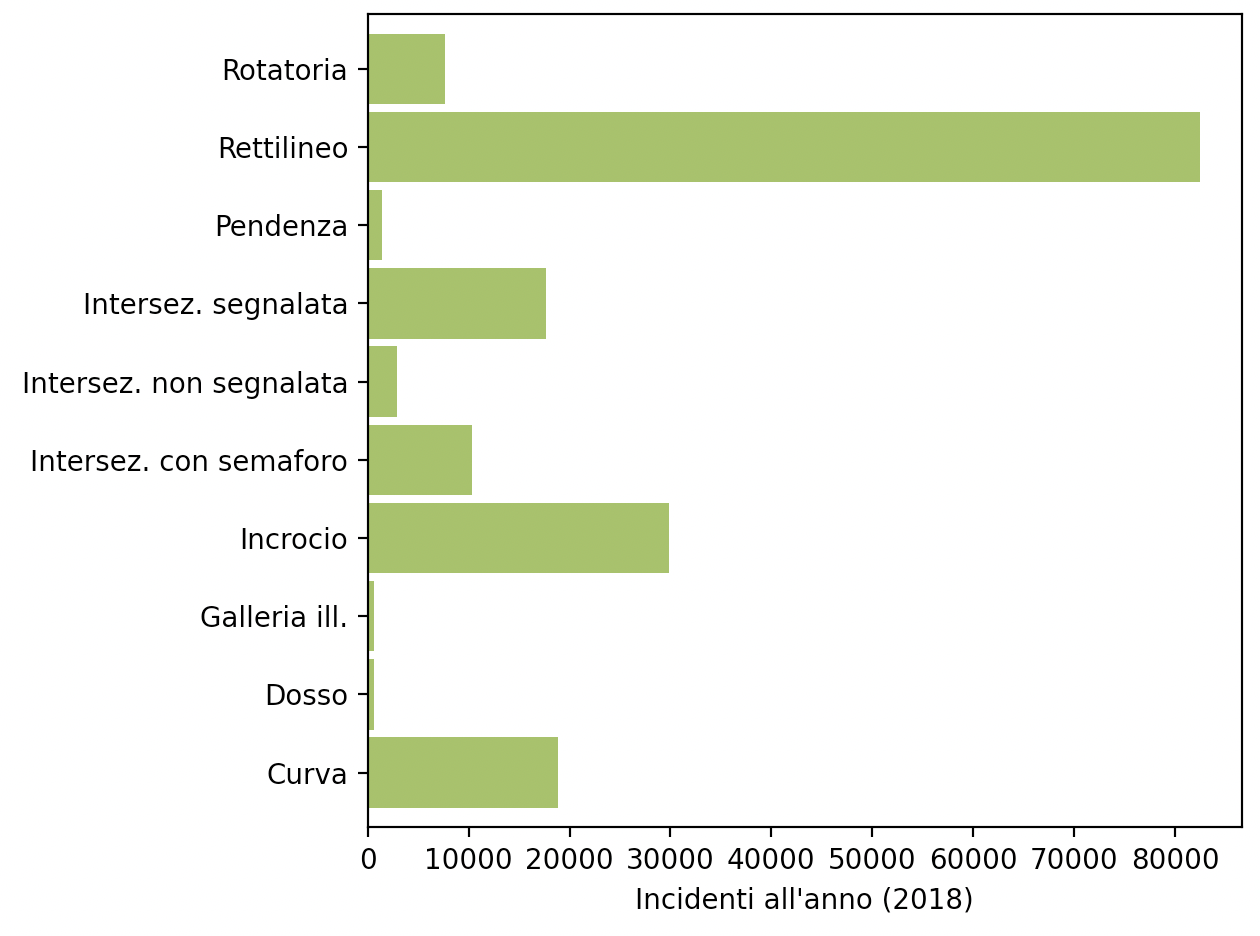
\includegraphics[width=0.5\linewidth]{../src/incidenti/incidenti_senza_coords/localizzazione_incidente/intersezioni.png}
    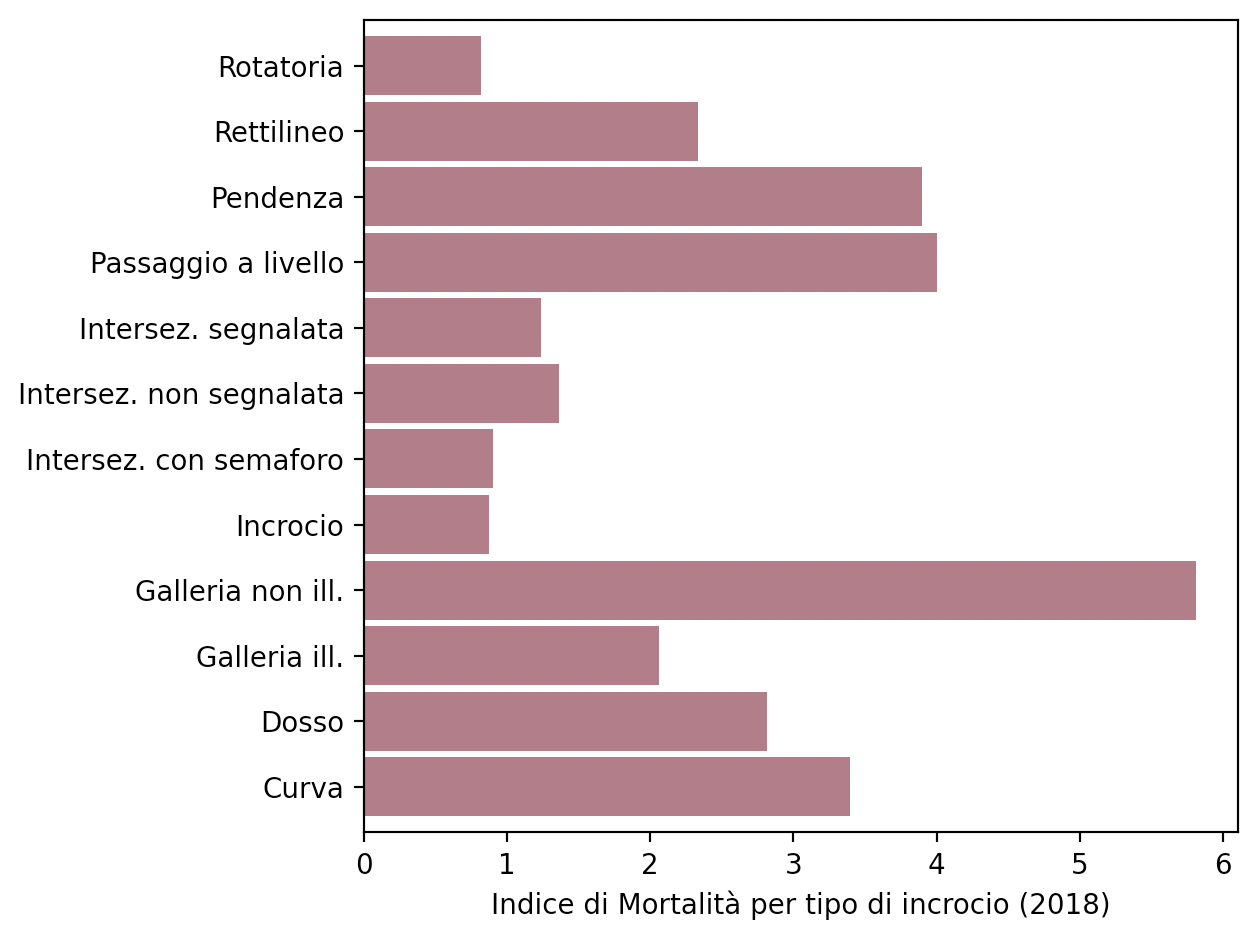
\includegraphics[width=0.5\linewidth]{../src/incidenti/incidenti_senza_coords/localizzazione_incidente/indice_mortalita.png}
    \caption{Percentuale di incidenti e rispettivo indice di mortalità per tipo di incrocio}
    \label{fig:tipo-intersezioni}
\end{figure}

L'indice di mortalità per tipologia di incrocio, raffigurato nel grafo destro 
dell'immagine \ref{fig:tipo-intersezioni}, mostra che, per quanto i rettilinei 
siano le zone in cui avvengono sinistri più frequentemente, non sono le zone 
con incidenti più pericolosi. 

Nella tabella sottostante sono riportati i valori, sia dell'indice di mortalità, 
sia dell'indice di feriti per tipologia di strada in cui è avvenuto l'incidente.

\begin{center}
    $Indice\_Mortalita\_Strada\_X = \displaystyle \frac{Numero\_Morti\_Strada\_X}{Numero\_Incidenti\_Strada\_X} * 100$ 
\end{center}

\begin{center}
    $Indice\_Feriti\_Strada\_X = \displaystyle \frac{Numero\_Feriti\_Strada\_X}{Numero\_Incidenti\_Strada\_X} * 100$ 
\end{center}

\begin{center}
    \def\arraystretch{1.5}%  
    \begin{tabular}{ |c|c|c| } 
    \hline
    Tipo di Incrocio & Indice Mortalità & Indice Feriti \\ 
    \hline
    \rowcolor{TableGray}
    Incrocio                & 0.88 & 143.10 \\
    Rotatoria               & 0.82 & 127.22 \\
    \rowcolor{TableGray}
    Intersez. segnalata     & 1.24 & 142.14 \\
    Intersez. con semaforo  & 0.9 & 147.05 \\
    \rowcolor{TableGray}
    Intersez. non segnalata & 1.36 & 139.97\\
    Passaggio a livello     & 4.0 & 134.67\\
    \rowcolor{TableGray}
    Rettilineo              & 2.33 & 138.94\\
    Curva                   & 3.39 & 145.26\\
    \rowcolor{TableGray}
    Dosso                   & 2.82 & 156.49\\
    Pendenza                & 3.9 & 134.10\\
    \rowcolor{TableGray}
    Galleria ill.           & 2.06 & 165.87\\
    Galleria non ill.       & 5.81 & 132.59\\
    \hline
    \end{tabular}
\end{center}

Per controllare la validità degli indici calcolati, si è ricavata la correlazione 
tra indice di mortalità, feriti e tra questi ultimi e il numero di incidenti per 
luogo.
I valori sono riportati nella tabella sottostante: 

\begin{center}
    \def\arraystretch{1.5}%  
    \begin{tabular}{ |c|c| }
        \hline
        \rowcolor{TableGray}
        Tra morti e feriti      & 0.96 \\ 
        Tra incidenti e feriti  & 0.99 \\
        \rowcolor{TableGray}
        Tra incidenti e morti   & 0.96 \\
        \hline
    \end{tabular}
\end{center}

Ne risulta che tutti gli insiemi siano linearmente correlati tra loro. 
Dalla tabella contenente l'indice di feriti, non è possibile dedurre molto, 
in quanto questo indicatore è molto simile tra tutte le categorie.

Per quanto riguarda invece, l'indice di mortalità, è chiaro che sia più alto 
per categorie di incidenti che avvengono ad alte velocità, come vicino a dossi, 
curve e gallerie, rispetto a tratti di strada, come incroci e semafori, 
dove le automobili stanno ripartendo.

%\clearpage
\subsection{Le tipologie di incidenti che provocano più feriti}

Il dataset Istat contiene informazioni riguardanti il numero di persone coinvolte 
in incidenti, in particolare l'età, il sesso e l'esito, cioè lo stato del passeggero 
dopo l'incidente, incolume, ferito, morto entro 24 ore o morto entro un mese.
Sarebbe interessante controllare se esistano tipologie di incidenti che provocano 
un maggior numero di feriti.

\begin{figure}
    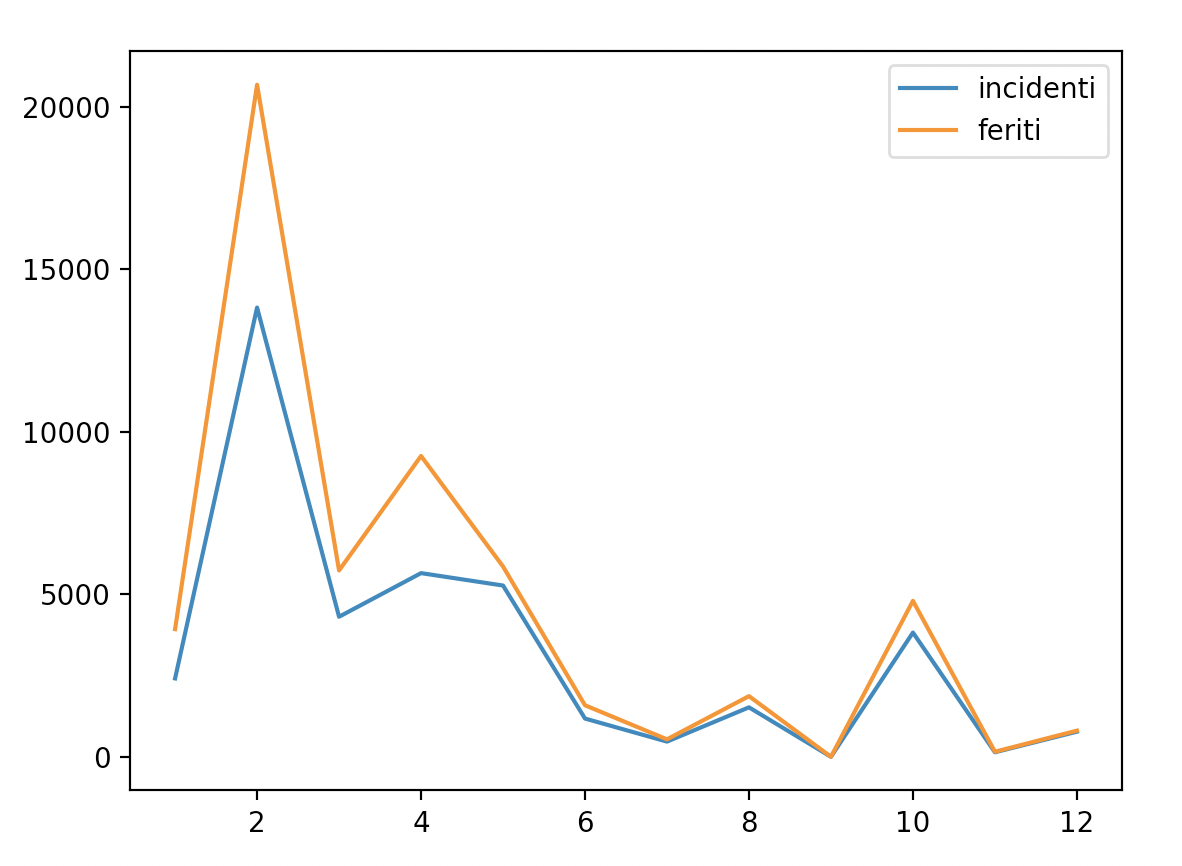
\includegraphics[width=\linewidth]{../src/incidenti/incidenti_senza_coords/natura_incidente/natura_incidente.png}
    \caption{Numero di feriti in base alla natura dell'incidente}
    \label{fig:numero-feriti}
\end{figure}

Nella figura \ref{fig:numero-feriti} si deduce che esistono tipologie di sinistri 
che favoriscono la presenza di un solo ferito, come gli sbandamenti. 
\'E possibile arrivare a questa conclusione perchè il numero di incidenti con 
un solo ferito, nella colonna \columnstyle{sbandamento} è tra i più alti, 
mentre la stessa categoria con due persone ferite ha volume molto più basso.
Al contrario, in incidenti come \columnstyle{tamponamento}, sono molto frequenti 
per ogni numero di feriti, il che fa pensare che semplicemente avvenga un alto numero 
di questo tipo di sinistro.

Le percentuali di osservazione di uno degli incidenti nel grafo sono riportate 
nella tabella sottostante\footnote{La somma delle percentuali dei tipi di 
incidenti dovrebbe ammontare a 1, ma sono state riportate solo quattro categorie, 
e non tutte.}: 

\begin{center}
    \def\arraystretch{1.5}%  
    \begin{tabular}{ |c|c| } 
    \hline
    Incidente & Percentuale del tipo \\ 
    \hline
    \rowcolor{TableGray}
    Sbandamento       & 0.097 \\
    Tamponamento      & 0.143 \\
    \rowcolor{TableGray}
    Scontro frontale  & 0.061 \\
    Urto con ostacolo & 0.039 \\
    \hline
    \end{tabular}
\end{center}

Avendo a disposizione il volume di incidenti per categoria, è possibile capire 
se il comportamento visibile nel grafo è dovuto al numero di sinistri. 

\begin{figure}
    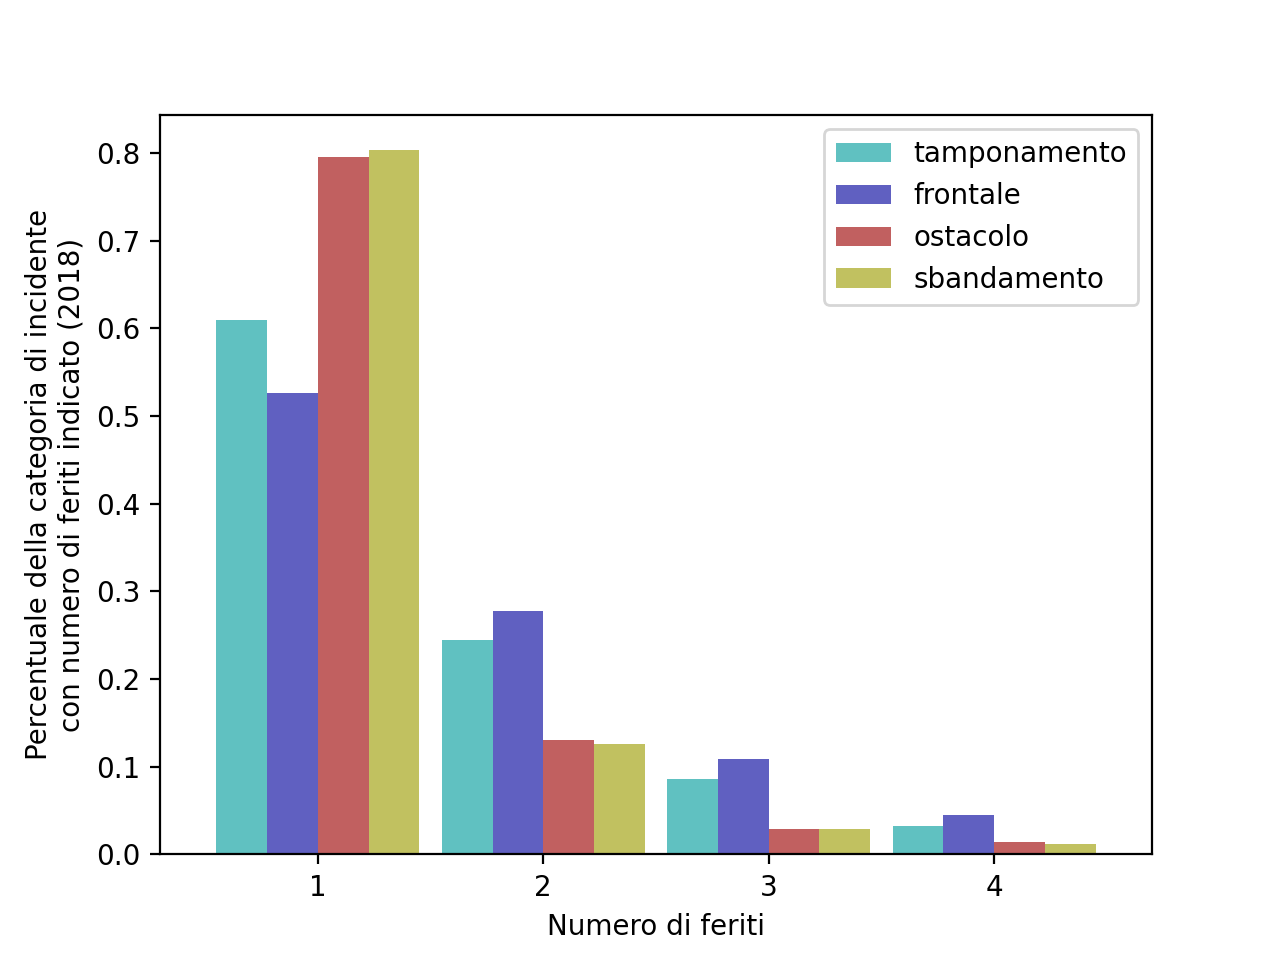
\includegraphics[width=\linewidth]{../src/incidenti/incidenti_senza_coords/natura_incidente/perc_natura_incidente.png}
    \caption{Percentuale del tipo di incidente, diviso per numero di feriti presenti}
    \label{fig:perc-numero-feriti}
\end{figure}

La figura \ref{fig:perc-numero-feriti} mostra la percentuale della categoria 
di incidenti, divisi per numero di feriti, dunque, sommando i valori delle 
colonne di colore uguale si ottiene $1.0$.

Avendo delle percentuali corrette in base al volume della categoria di incidente, 
si osserva come alcune tipologie, come urto con ostacolo e sbandamento, 
favoriscano una sola persona ferita, mentre altre, come i tamponamenti e 
gli scontri frontali, abbiano una maggiore percentuale di 
incidenti con più di un ferito.

%\clearpage
\subsection{Incroci che favoriscono incidenti con pedoni}

Il dataset Istat fornisce informazioni riguardanti i pedoni coinvolti in un incidente, 
si potrebbe controllare se esistono tipologie di incrocio che coinvolgono un 
alto numero di persone a piedi.

La figura \ref{fig:pedoni-intersezioni} mostra il numero di incidenti, 
ordinati in base alla tipologia di intersezioni e al numero di persone coinvolte.

\begin{figure}
    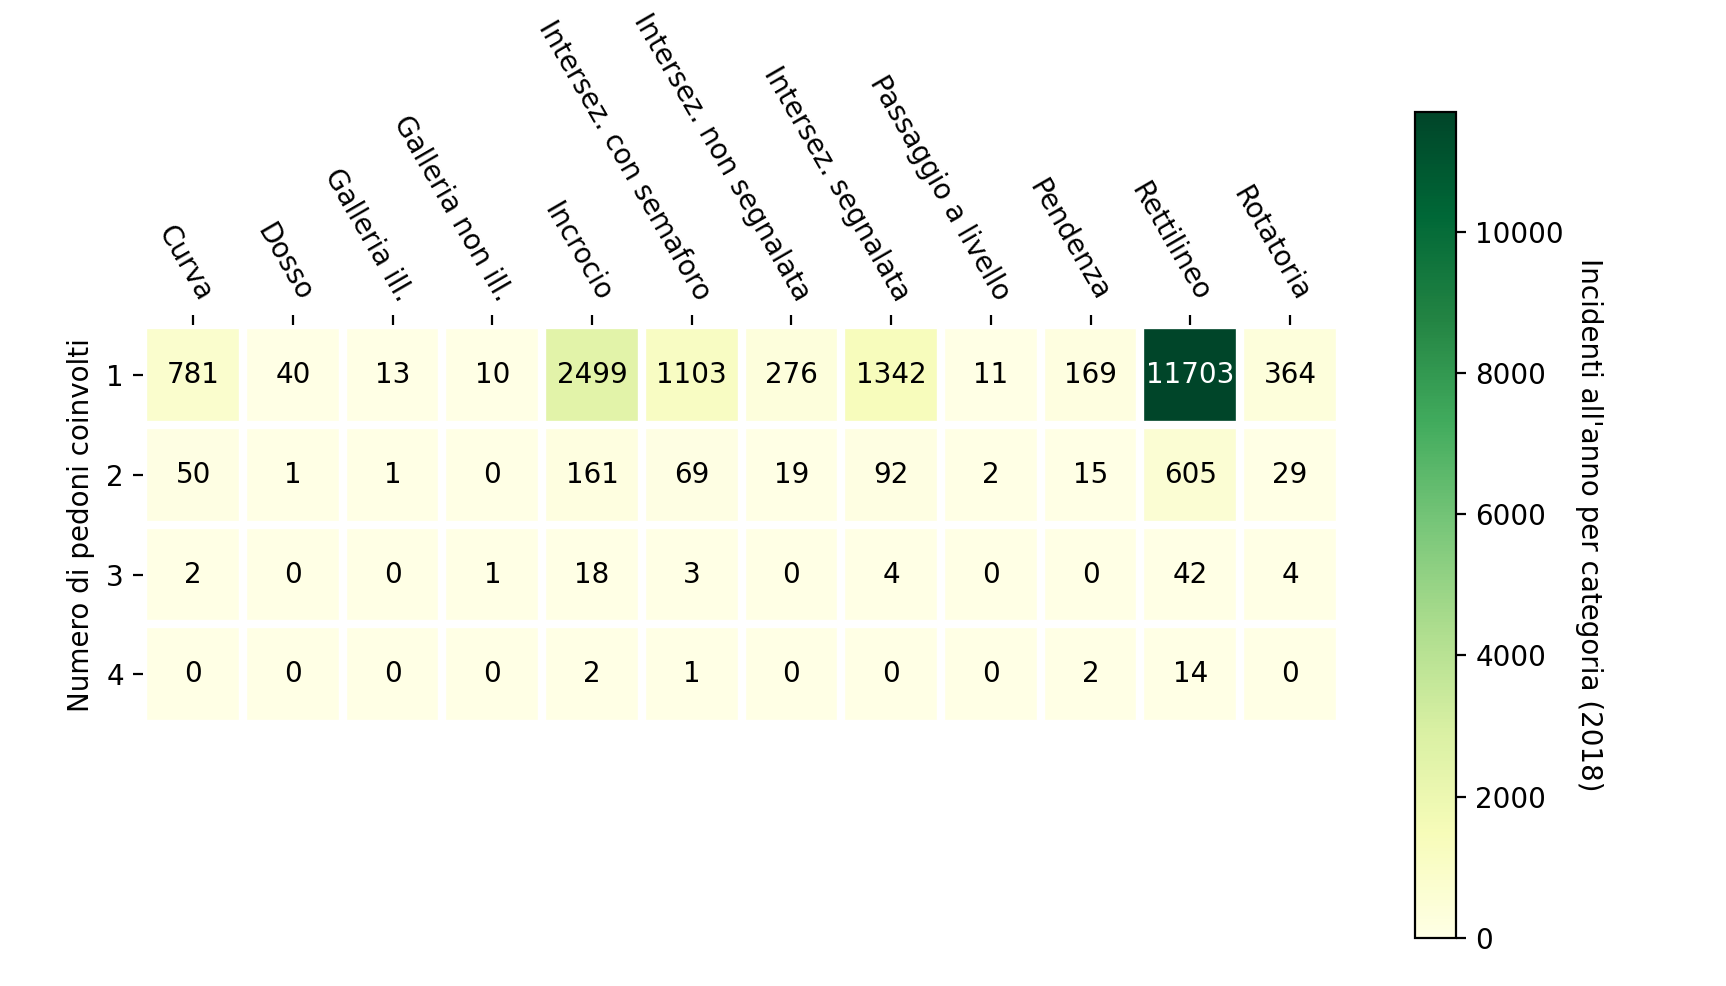
\includegraphics[width=\linewidth]{../src/incidenti/incidenti_senza_coords/pedoni/pedoni_incroci.png}
    \caption{Tipologia di intersezioni e pedoni coinvolti}
    \label{fig:pedoni-intersezioni}
\end{figure}

Similmente a come si era visto nel grafo\ref{fig:tipo-intersezioni}, nella nuova 
figura spicca un alto numero di rettilinei.
\'E possibile che per la maggior parte, questo outlier sia dovuto all'alto 
numero di tratti di strada dritti, tuttavia, se si confrontano le due immagini, 
il numero di incidenti su rettilineo con pedoni coinvolti è quasi cinque 
volte il valore della seconda posizione.

Questo alto numero di incidenti fa pensare che esista un qualche fattore 
che comporta maggiore coinvolgimento di pedoni lungo i rettilinei, come per 
esempio, l'alta velocità dei veicoli.

\begin{figure}
    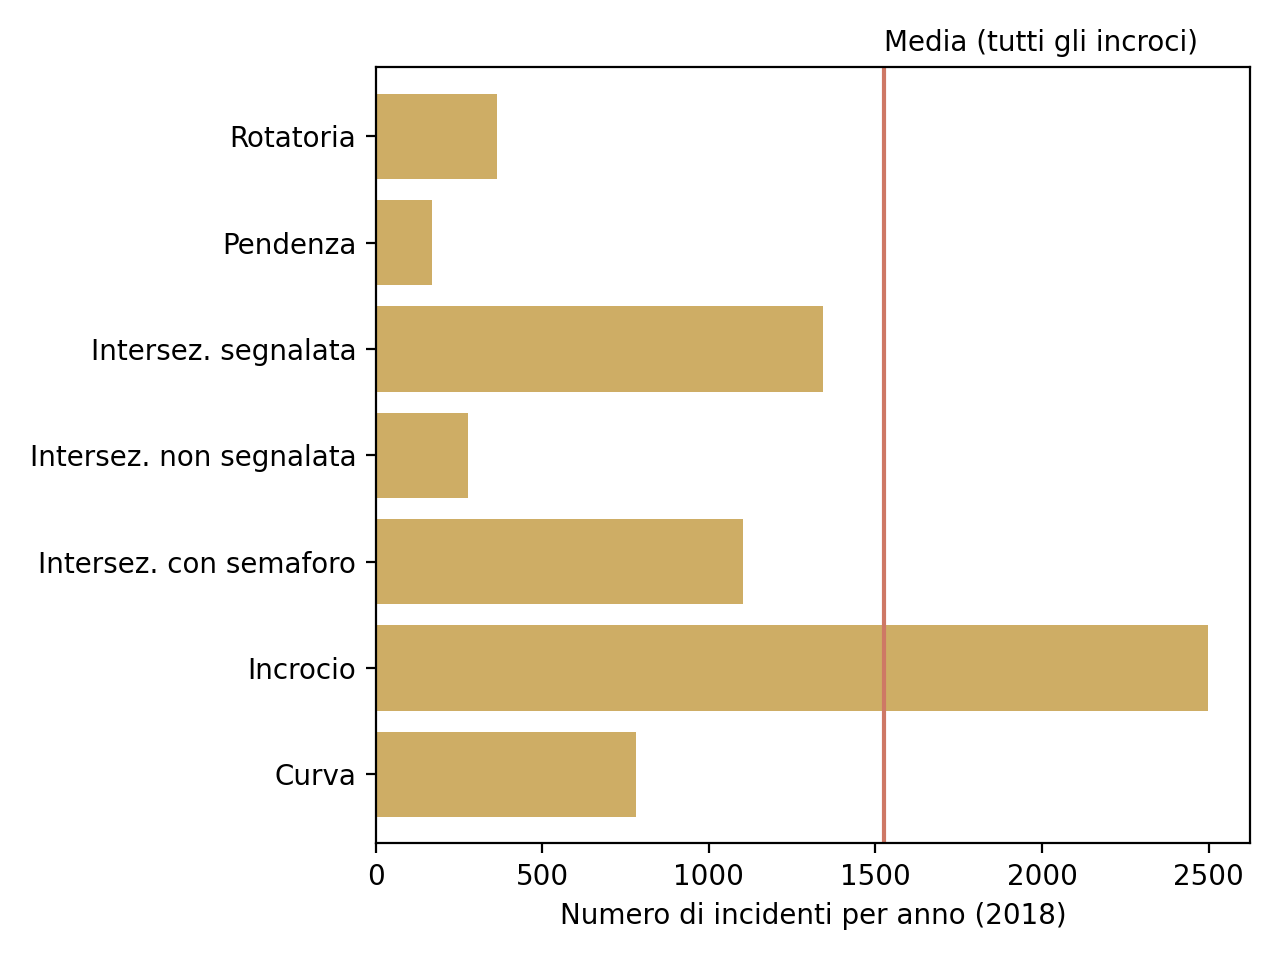
\includegraphics[width=\linewidth]{../src/incidenti/incidenti_senza_coords/pedoni/pedoni_no_rett.png}
    \caption{Tipologia di intersezioni e pedoni coinvolti, ignorando le categorie con valori più bassi}
    \label{fig:pedoni-no-rett}
\end{figure}

In figura \ref{fig:pedoni-no-rett} sono state escluse le categorie con minore 
valore\footnote{Sono state rimosse tutte le categorie con valore minore di 
150 incidenti all'anno}, 
in particolare \columnstyle{Dosso}, \columnstyle{Galleria ill.}, 
\columnstyle{Galleria non ill.,} e \columnstyle{Passaggio a livello}.
Il grafo ottenuto è più bilanciato, con \columnstyle{incroci} e 
\columnstyle{intersezioni non segnalate} che spiccano come tipi di strada con 
maggiore coinvolgimento di pedoni, ovviamente dopo \columnstyle{rettilineo}, 
e le restanti categorie non troppo distanti.
Va specificato che il grafo \ref{fig:pedoni-no-rett} sia stato realizzato con 
una scala logaritmica, poichè il numero di pedoni coinvolti su rettilineo è un 
ordine di grandezza maggiore rispetto alla media.

A differenza della precedente analisi sui tratti di strada più pericolosi, 
l'immagine dipinta in questo capitolo è molto diversa.
In questo caso, non si può più dire che i tratti più pericolosi siano quelli 
che favoriscono alte velocità, ma sembra che il maggior numero di pedoni 
siano coinvolti in incroci e zone in cui la visibilità è ostruita, come le curve.

%\clearpage
\subsection{Età dei pedoni coinvolti in incidenti}

\'E scontato che, se coinvolti in un incidente, un pedone di venti anni non ha la stessa 
probabilità di essere ferito rispetto a una persona di settanta.
\'E possibile osservare questo comportamento utilizzando i dati che si ha a disposizione?

Per prima cosa si sono utilizzati i campi \columnstyle{età\_pedone} per creare un grafo 
in cui sia visibile il numero di pedoni feriti e morti, divisi per fascia di età.

\begin{figure}
    \includegraphics[width=\linewidth]{../src/incidenti/incidenti_senza_coords/pedoni/eta_pedoni_iniziale.png}
    \caption{Fasce di età dei pedoni coinvolti in incidenti}
    \label{fig:eta-pedoni-iniziale}
\end{figure}

Dal grafo \ref{fig:eta-pedoni-iniziale} si osserva che la fascia di età più colpita 
è quella dei \columnstyle{65+} anni, tuttavia esiste un secondo picco, nel grafo dei 
pedoni feriti, che  comprende le fasce tra trenta e cinquantaquattro anni di età.

\begin{figure}
    \includegraphics[width=\linewidth]{../src/incidenti/incidenti_senza_coords/pedoni/eta_pedoni.png}
    \caption{Fasce di età dei pedoni coinvolti in incidenti, normalizzate per numero di anni 
    presenti nella fascia}
    \label{fig:eta-pedoni}
\end{figure}

Non tutte queste fasce però contengono lo stesso numero di anni di età, 
per esempio \columnstyle{30-44} contiene quindici anni, mentre 
\columnstyle{18-20} ne contiene solo due.

\begin{lstlisting}[language=Python]
    numero_anni = np.array([5, 5, 5, 3, 10, 15, 10, 10, 20])

    pedoni_feriti_vals = pedoni_feriti.values / numero_anni
    pedoni_morti_vals = pedoni_morti.values / numero_anni
\end{lstlisting}

Se si normalizza per anni contenuti in ogni fascia, ipotizzando un numero 
costante di persone di ogni età\footnote{La normalizzazione tiene conto 
che la fascia di età \columnstyle{65+} valga venti anni.}, 
si ottiene un grafo, visibile in figura \ref{fig:eta-pedoni}, che, per 
quanto riguarda i pedoni feriti, è molto differente.
Ignorando gli individui più giovani, tutte le altre fasce sono coinvolte 
in modo omogeneo, con un picco nella categoria \columnstyle{65+ anni}.
D'altra parte, il grafo destro, contenente i pedoni morti per fascia di età, 
non subisce un grande cambiamento, mantenendo il punto di massimo con 
i pedoni più anziani.

Non è detto, tuttavia, che in Italia il numero di individui con 
la stessa età sia costante anzi, le percentuali di individui per fascia, 
trovate sul sito Tuttitalia \cite{TUTTITALIA:1}, riportate nella tabella 
sottostante, non sono particolarmente omogenee: 

\begin{center}
    \def\arraystretch{1.5}%  
    \begin{tabular}{ |c|c| } 
    \hline
    Fascia & Percentuale Popolazione \\ 
    \hline
    \rowcolor{TableGray}
    0-5     & 3.9 \% \\ 
    6-9     & 4.5 \% \\
    \rowcolor{TableGray}
    10-14   & 4.8 \% \\
    15-17   & 3.1 \% \\
    \rowcolor{TableGray}
    18-20   & 2.8 \% \\ 
    21-24   & 4   \% \\
    \rowcolor{TableGray}
    25-29   & 5.3 \% \\
    30-44   & 19  \% \\
    \rowcolor{TableGray}
    45-54   & 18.2\% \\ 
    55-59   & 7.3 \% \\
    \rowcolor{TableGray}
    60-64   & 6.4 \% \\
    65$+$   & 19.3\% \\
    \hline
    \end{tabular}
\end{center}

Per poter essere utilizzate, le fasce trovate sono state sommate, e in alcuni casi 
si è dovuto stimare la percentuale di popolazione con determinata età in 
quanto si sarebbe dovuto dividere una fascia.
Un esempio di questa divisione è la fascia dei \columnstyle{15-19} anni presente nei 
dati della fonte. 
I dati Istat hanno invece una categoria \columnstyle{15-17} anni e un'altra 
\columnstyle{18-29} anni. 
\'E dunque necessario spostare i diciotto e i diciannovenni dalla prima alla 
seconda fascia. 
In questi casi, si è semplicemente assunto che il numero di individui sia omogeneamente 
diviso per età, cioè nella fascia \columnstyle{15-19} si ha lo stesso numero di 
persone con quindici e sedici anni.
Seguendo questa logica, per spostare i due anni di età nella categoria successiva, 
si divide la percentuale di \columnstyle{15-19} per cinque e si moltiplica per due. 
Il risultato ottento lo si aggiunge alla fascia \columnstyle{18-29}.

\begin{lstlisting}
    correct_order =         ['0-5  ', '6-9  ', '10-14', '15-17', '18-29', '30-44', '45-54', '55-64','65+  ']
    perc_fascia = np.array( [3.9, 4.5, 4.8, 3.1, 12.1, 19, 18.2, 13.7, 19.3]) / 100

    pedoni_feriti_vals = pedoni_feriti.values / perc_fascia
    pedoni_morti_vals = pedoni_morti.values / perc_fascia
\end{lstlisting}

\begin{figure}
    \includegraphics[width=\linewidth]{../src/incidenti/incidenti_senza_coords/pedoni/eta_pedoni_norm.png}
    \caption{Fasce di età dei pedoni coinvolti in incidenti, normalizzate tramite percentuale di popolazione}
    \label{fig:eta-pedoni-norm}
\end{figure}

Una volta aver corretto l'immagine precendente, 
si ottiene la figura \ref{fig:eta-pedoni-norm} dove, soprattutto 
nel grafo di destra, è presente una curva particolarmente alta 
nelle fasce più anziane, e un secondo picco nella categoria \columnstyle{18-29 anni}.
Anche nel grafo di sinistra è presente la stessa impennata in corrispondenza 
della seconda fascia, mentre la categoria \columnstyle{65+} non 
risulta particolarmente alta.

L'incremento di morti nelle fasce più anziane, si può speculare sia dovuto al 
fatto che questi ultimi siano più propensi all'essere feriti in un incidente. 
Mentre, per la prima categoria, può essere che, soprattutto tra i più giovani, 
si preferisca ancora muoversi a piedi invece che in macchina.

\subsection{Età dei conducenti coinvolti in incidenti}

Avendo a disposizione le informazioni riguardanti l'età del conducente del 
veicolo che ha causato l'incidente, è possibile controllare se esistono fasce di 
età con incidentalità particolarmente alta.

\begin{figure}
    \includegraphics[width=\linewidth]{../src/incidenti/incidenti_senza_coords/mortalita/indice_mortalita_eta.png}
    \caption{Indice di mortalità degli incidenti, divisi in base all'età del conducente}
    \label{fig:indice-mortalita-eta}
\end{figure}

In primo luogo, il grafo destro nella figura \ref{fig:indice-mortalita-eta} contiene 
la percentuale, per fascia di età del conducente, di incidenti totali commessi, insieme 
al numero di morti in questi incidenti\footnote{Ogni colonna contiene incidenti in 
cui il conducente rientra nella fascia di età, la persona deceduta tuttavia potrebbe non 
essere il conducente}.

In particolare, più di un quarto degli incidenti totali coinvolgono conducenti nella 
fascia d'età \columnstyle{30-44} mentre, probabilmente per il basso numero di 
guidatori nella fascia \columnstyle{15-17}, questo gruppo sembra essere molto 
più responsabile alla guida.

Nel grafo di sinistra in figura \ref{fig:indice-mortalita-eta}, invece, 
è rappresentato l'indice di mortalità di questi incidenti, 
calcolato utilizzando la formula: 

\begin{center}
    $Indice\_Mortalita\_X = \displaystyle \frac{Numero\_Morti\_X}{Numero\_Incidenti\_X} * 100$ 
\end{center}

L'indice di mortalità presente nel grafo aumenta all'aumentare dell'età, 
e il risultato trovato sembra essere confermato dalla stima realizzata nello studio 
ACI del 2018 sugli incidenti stradali \cite{ACI:3}. 

Tuttavia, come già spiegato nella sezione precedente, la prima fascia di cui si è parlato 
contiene quindici anni, mentre la seconda solamente due. Sarebbe quindi opportuno 
normalizzare la percentuale di incidenti commessi, con una stima del numero di 
guidatori nella rispettiva fascia di età.

\begin{lstlisting}
    perc_fascia = np.array( [3.1, 12.2, 19, 18.2, 13.7, 19.3]) / 100

    incidenti_per_eta /= perc_fascia
    morti_per_eta /= perc_fascia

    indice_mortalita = morti_per_eta * 100 / incidenti_per_eta
\end{lstlisting}

\begin{figure}
    \includegraphics[width=\linewidth]{../src/incidenti/incidenti_senza_coords/mortalita/indice_mort_norm.png}
    \caption{Indice di mortalità degli incidenti, normalizzato per popolazione standard}
    \label{fig:indice-mort-norm}
\end{figure}

Una volta normalizzato per la popolazione standard in Italia, il numero di incidenti per 
fascia di età, nel grafo destro della figura \ref{fig:indice-mort-norm}, mostra che le 
età nelle quali si commettono più sinistri sono quelle dei \columnstyle{18-29 anni}, 
con un calo nei valori successivi.
D'altra parte, l'indice di mortalità non cambia, poichè è un rapporto in cui i fattori 
sono stati divisi per costanti uguali per ogni fascia.

%\clearpage
\section{Dati ACI}

I dati trovati sul sito di ACI sono inizialmente divisi in due categorie in 
base al tipo di strada dove l'incidente è avvenuto, 
su autostrade o strade provinciali.
I due gruppi, a loro volta sono rispettivamente divisi in file, a seconda 
dell'informazione contenuta, come incidenti con località, incidenti per 
comune, per mese, per giorno della settimana o ora.

\subsection{Incidenti per regione}

Utilizzando i dati ACI, in particolare i file \columnstyle{localizzazione}, è 
possibile dividere gli incidenti per regione e per provincia.
Grazie al dataset geojson di Guglielmo 
Celata\footnote{\url{https://github.com/openpolis/geojson-italy}}, 
è stato possibile realizzare le mappe in figura \ref{fig:incidenti-per-regione}, 
che raffigurano rispettivamente, le regioni con più incidentalità nel per ogni 
anno nelle strade provinciali e nelle autostrade, nell'anno 2018.

Ovviamente il Nord Italia ha il primato per quanto riguarda gli incidenti, 
soprattutto nelle regioni di Lombardia, Veneto e Emilia Romagna. 
Spicca poi il Lazio, dove la maggior parte degli incidenti avvengono su autostrade, 
in quanto il volume di incidenti è nella media nella prima mappa in figura 
\ref{fig:incidenti-per-regione}, mentre è il massimo annuale nella seconda mappa.

\begin{figure}
    \includegraphics[width=0.5\linewidth]{../src/incidenti/incidenti_aci/mappe_regioni/incidenti_regione.png}
    \includegraphics[width=0.5\linewidth]{../src/incidenti/incidenti_aci/mappe_regioni/incidenti_regione_autostrade.png}
    \caption{Incidenti su autostrade e su strade provinciali nel 2018}
    \label{fig:incidenti-per-regione}
\end{figure}

Per quanto riguarda, invece, il numero di incidenti per ogni anno, 
dalla heatmap \ref{fig:regione-heatmap} 
si nota che non cambia molto di anno in anno, e le regioni con maggiore numero 
di incidenti rimangono sempre Lombardia e Veneto.

Per controllare le tendenze di incremento e decremento di incidenti per regione, 
si è calcolata la deviazione standard per ogni regione\footnote{Deviazione standard: 
misura della distanza dei dati di un campione dalla media\cite{PROB_E_STATISTICA:2}}.
Risulta che la regione con maggiore cambiamento di incidenti di anno in anno 
è il Lazio, con $324$ incidenti l'anno, mentre quella con minore 
variazione è la Valle d'Aosta, con $8$.

\begin{figure}
    \includegraphics[width=\linewidth]{../src/incidenti/incidenti_aci/mappe_regioni/regioni_heatmap.png}
    \caption{Incidenti all'anno per regione su strade provinciali}
    \label{fig:regione-heatmap}
\end{figure}

I grafi precedenti, soprattutto le heatmap regionali, non tengono conto del 
volume del traffico.
Non avendo informazioni riguardanti il traffico in tutta Italia, si sono stimate 
queste informazioni tramite il numero di patentati per regione.
Una stima eseguita con il numero di patentati per regione, non è molto accurata, 
in quanto molte persone patentate in una regione, possono lavorare in altre, e 
influire in modo errato al conteggio degli incidenti. 

\begin{figure}
    \includegraphics[width=\linewidth]{../src/incidenti/incidenti_aci/mappe_regioni/incidenti_patenti_italia.png}
    \caption{Incidenti e patentati per regione}
    \label{fig:incidenti-patentati}
\end{figure}

Se si visualizza il rapporto tra incidenti e patentati per regione 
(figura \ref{fig:incidenti-patentati}), si osserva una chiara distinzione 
tra Nord, Centro e Sud Italia. 
A cosa è dovuta questa ampia disparità?

Nella seguente tabella sono riportate le medie di incidenti annuali per regione, 
e quella di patentati per regione.

\begin{center}
    \def\arraystretch{1.5}%  
    \begin{tabular}{ |c|c|c| } 
    \hline
    Zona & Media di Incidenti annuali & Patentati (in Milioni) \\ 
    \hline
    \rowcolor{TableGray}
    Nord    &   2470 &   2.28 \\ 
    Centro  &   2395 &   1.97 \\ 
    \rowcolor{TableGray}
    Sud     &   1145 &   1.57 \\ 
    \hline
    \end{tabular}
\end{center}

Il grafo \ref{fig:incidenti-patentati-bar} è stato suddiviso tra regioni del nord, 
centro e sud, per facilitare la lettura, e indica le percentuali di incidenti e 
patentati per la rispettiva regione. 
\'E subito osservabile che, nella maggior parte delle regioni del centro, 
la percentuale di incidenti supera quella di patentati, 
mentre nel Sud Italia accade il fenomeno opposto.

\begin{figure}
    \includegraphics[width=\linewidth]{../src/incidenti/incidenti_aci/mappe_regioni/incidenti_patenti_bar.png}
    \caption{Incidenti e patentati per regione}
    \label{fig:incidenti-patentati-bar}
\end{figure}

\begin{figure}
    \includegraphics[width=\linewidth]{../src/incidenti/incidenti_aci/mappe_regioni/incidenti_patenti_box.png}
    \caption{Incidenti e patentati per Nord, Centro e Sud Italia}
    \label{fig:incidenti-patentati-box}
\end{figure}

La figura \ref{fig:incidenti-patentati-box} permette di capire il motivo della disparità 
tra centro e Sud Italia.
Al sud, il numero di incidenti è molto minore rispetto al centro Italia, mentre, 
sempre le stesse due zone, il numero di patentati non cambia molto. 
\'E ovvio che tenendo il denominatore costante, il numero minore di incidenti al 
sud causa una frazione minore.

Quali potrebbero essere le motivazioni di questa disparità?
Come già accennato in precendenza, una delle motivazioni principali 
deve essere la destinazione lavorativa della popolazione, tuttavia va anche sottolineato 
la precisione del numero di patenti come stimatore del traffico non è da considerarsi 
particolarmente attendibile.

\subsection{Differenze tra mesi estivi e invernali}

Sarebbe interessante controllare se i dati ACI confermano le tendenze trovate tramite 
le informazioni Istat, e vedere se al sud, il numero di incidenti cresce 
come conseguenza delle vacanze estive.

\begin{figure}
    \includegraphics[width=\linewidth]{../src/incidenti/incidenti_aci/mappe_regioni/estate_inverno.png}
    \caption{Incidenti per regione nei mesi estivi e invernali}
    \label{fig:estate-inverno}
\end{figure}

Nella figura \ref{fig:estate-inverno}, sono rappresentati i numeri di incidenti presenti 
in mesi invernali e estivi, divisi per regione.

In tutte le regioni italiane, il numero di incidenti in estate è maggiore del 
numero di incidenti in inverno. 
La probabile motivazione di ciò probabilmente il fatto che 
le persone si muovono meno nei mesi freddi, rispetto a quelli caldi.

Il comportamento che si stava cercando, cioè più incidenti in estate nel 
Sud Italia, non è visibile. 
Un modo in cui si potrebbe ricavarlo, però, è osservare gli incidenti sulle autostrade 
principali in Agosto.
Questo tipo di controllo verrà eseguito in un capitolo successivo.


\subsection{Incidenti per provincia}

Utilizzando, ancora una volta, i file geojson contenenti i limiti delle province, è 
possibile creare delle heatmap raffiguranti quali tra queste hanno maggior numero 
di incidenti.

Il calcolo, avendo a disposizione dati riguardanti strade provinciali e autostrade, 
è stato realizzato per entrambi i casi.

\begin{figure}
    \includegraphics[width=0.5\linewidth]{../src/provincia/lombardia_autostrade.png}
    \includegraphics[width=0.5\linewidth]{../src/provincia/lombardia_strade_prov.png}
    \caption{Incidenti nelle autostrade e nelle strade provinciali in Lombardia}
    \label{fig:lombardia-strade}
\end{figure}

Nella figura \ref{fig:lombardia-strade} sono mostrati gli incidenti in Lombardia, 
avvenuti rispettivamente nelle autostrade e nelle strade provinciali.
In entrambi i casi, si nota che la provincia di Milano è quella caratterizzata da 
un maggior numero di incidenti. 
D'altra parte, per quanto riguarda le differenze, nelle province di Bergamo e Como, 
i sinistri crescono molto nelle strade provinciali rispetto alle autostrade.

Viene riportato lo stesso calcolo, per le province del Lazio.

\begin{figure}
    \includegraphics[width=0.5\linewidth]{../src/provincia/lazio_autostrade.png}
    \includegraphics[width=0.5\linewidth]{../src/provincia/lazio_strade_prov.png}
    \caption{Incidenti nelle autostrade e nelle strade provinciali nel Lazio}
    \label{fig:lazio-strade}
\end{figure}

Nella figura \ref{fig:lazio-strade} raffigurante il Lazio, va specificato che il numero 
di incidenti su autostrade è molto più alto rispetto a quello su strade provinciali, 
fenomeno già osservato nella mappa \ref{fig:incidenti-per-regione}.

Inoltre, la provincia di Frosinone ha un numero particolarmente alto di incidenti su 
autostrade, mentre la provincia di Latina, al contrario, ha un maggiore incremento di 
sinistri su strade provinciali.

Non è difficile trovare il perchè di questi numeri, in quanto l'autostrada A01 passa 
attraverso la provincia di Frosinone e non quella di Latina.

%\clearpage
\subsection{Le strade pericolose in provincia di Milano}

\'E anche possibile approfondire, allo stesso modo del calcolo degli incidenti per 
provincia, calcolando quali sono le strade più pericolose, per esempio, 
a Milano.

Utilizzando il sito Geojson.io\footnote{\url{https://geojson.io/}}, 
è stato possibile tracciare i percorsi delle principali autostrade in prossimità di 
Milano. Il risultato è visibile nella figura \ref{fig:line-incidenti-milano}.

\begin{figure}
    \includegraphics[width=\linewidth]{../src/incidenti/incidenti_aci/autostrade/incidenti_line_chart.png}
    \caption{Autostrade con più incidenti nel 2018}
    \label{fig:line-incidenti-milano}
\end{figure}

In particolare, dalla mappa \ref{fig:line-incidenti-milano}, si deduce che le 
Tangenziali Ovest e Est, e l'autostrada Torino-Trieste, sono i tratti di 
strada con più incidenti.

Infine, se si avesse a disposizione la posizione precisa degli incidenti, 
sarebbe possibile anche dividere queste tratte pericolose, in sezioni più piccole, 
e controllare se esistano zone che alzano il volume di incidenti.

%\clearpage
\subsection{Esiste correlazione tra incidenti e feriti?}

Esiste correlazione tra morti e incidenti, o tra morti e feriti?
Ovviamente si attende un esito positivo a queste domande.
L'indice di correlazione utilizzato è il coefficiente di Pearson, calcolato tramite la 
formula: 

\begin{center}
    $\rho_{X, Y} = \displaystyle \frac{cov(X, Y)}{\sigma_X \sigma_Y}$
\end{center}

\begin{center}
    con: $\rho_{X, Y} \rightarrow [-1, 1]$
\end{center}

dove X e Y sono i due campioni di cui si vuole calcolare la correlazione, 
\methodstyle{cov()} è la covarianza, e $\sigma_X$ è la deviazione standard del 
campione X \cite{PROB_E_STATISTICA:3}.

Una volta divisi i dati, è possibile calcolare l'indice tramite il metodo 
\methodstyle{corr()}, i risultati sono riportati nella seguente tabella.

\begin{center}
    \def\arraystretch{1.5}%  
    \begin{tabular}{ |c|c|c| } 
    \hline
    Incidenti & Incidenti & Feriti \\ 
    Feriti & Morti & Morti \\ 
    \hline
    0.9836 & 0.3385 & 0.3355 \\ 
    \hline
    \end{tabular}
\end{center}

\begin{figure}
    \includegraphics[width=\linewidth]{../src/incidenti/incidenti_aci/provincia/corr_incidenti.png}
    \caption{Correlazione tra numero di feriti e incidenti nelle venti province con maggior numero di sinistri}
    \label{fig:corr-incidenti-feriti}
\end{figure}

Tracciando il grafo \ref{fig:corr-incidenti-feriti}, dei primi trenta valori 
del dataset ACI, è chiaramente visibile la correlazione tra 
numero di incidenti e numero di feriti, in quanto nella maggior parte dei casi, 
all'aumentare del numero di incidenti il numero di feriti cresce allo stesso modo.

L'unico dubbio che possa sorgere è che il numero di feriti sia maggiore del 
numero di incidenti, tuttavia controllando il dataset, ogni 
riga contiene un numero di feriti maggiore.
\'E possibile che il dataset contenga solo incidenti con almeno un ferito, 
e quindi ignori tutti i sinistri non particolarmente significativi.
D'altra parte, tenendo conto che si sono utilizzati dati raccolti lungo 
le autostrade, è possibile che la maggior parte dei sinistri comporti 
un alto numero di feriti. 
Nella tabella sottostante sono  mostrate le prime righe del dataset, con i 
rispettivi numeri di incidenti e feriti. 

\begin{center}
    \def\arraystretch{1.5}%  
    \begin{tabular}{ |c|c|c|c| } 
    \hline
    Provincia & Comune & Incidenti & Feriti \\ 
    \hline
    \rowcolor{TableGray}
    Torino & Brandizzo & 5 & 10\\
    Torino & Chivasso & 12 & 18\\
    \rowcolor{TableGray}
    Torino & Rondissone & 6 & 12\\
    Torino & Settimo Torinese & 25 & 40\\
    \hline
    \end{tabular}
\end{center}

Il coefficiente di Pearson, per quanto riguarda Incidenti e Feriti, 
è molto vicino a uno, quindi i due campioni sono strettamente correlati.
Nonostante, in generale, correlazione non implichi causa o effetto, cioè, non 
è detto che due fattori correlati si influenzino in alcun modo, in questo caso è 
difficile pensare che il numero di incidenti non sia alla causa del aumenare o diminuire 
del numero di feriti.
I coefficienti riguardanti i morti sono molto meno vicini a uno, probabilmente 
per il minor numero di incidenti mortali, che rendono il campione più ristretto.

\subsection{Le autostrade più pericolose}

Quali sono le autostrade con più incidenti durante l'anno? 
Sono tutte autostrade o ai primi posti ci sono anche delle strade statali? 

\begin{figure}
    \includegraphics[width=\linewidth]{../src/incidenti/incidenti_aci/autostrade/autostrade.png}
    \caption{Autostrade con più incidenti nel 2018}
    \label{fig:incidenti-autostrade}
\end{figure}

Nella figura \ref{fig:incidenti-autostrade} sono  raffigurate le autostrade con 
maggiore numero di incidenti nel 2018. 
Non è una sorpresa che le prime posizioni della lista coincidano 
anche con le strade più trafficate, come l'Autostrada del Sole e l'Adriatica.

Tuttavia sono anche presenti, due strade statali, SS1 e SS16. 
La motivazione dell'alto numero di incidenti su queste direttive, potrebbe essere 
la lunghezza di queste. Infatti entrambe sono strade che coprono la costa Italiana 
da nord a sud e, nella maggior parte della loro estensione, 
hanno solamente due corsie.

L'avere i sensi di marcia separati, e delle corsie designate al sorpasso, nel caso 
delle autostrade non può che essere un fattore che influenza negativamente 
il numero degli incidenti. 
D'altra parte, l'essere costretti a sorpassare sulla corsia adibita al senso di 
marcia opposto, nel caso della SS1 e SS16, porta possibilmente a un aumento dei 
sinistri.

\subsection{Le autostrade più utilizzate in estate cambiano a seconda dell'anno?}

Una domanda che sorge spontanea è se le autostrade con più incidenti 
cambino al cambiare dell'anno.
Una motivazione di questo fenomento potrebbe essere, il cambiamento 
delle mode riguadanti le località di vacanza.
Per esempio, nel 2018, le mete preferite sono state Puglia e 
Toscana\cite{INFOGRAFICA_ISTAT:1}, mentre nel 2019, oltre alla Puglia, 
una percentuale sostanziale di turisti si è recata in 
Emilia Romagna e Liguria\cite{REPORT_ISTAT_2019:1}.

Avendo a disposizione i dati di tutte le annate, dal 2010 al 2018, 
è anche possibile controllare se esistano anni con un volume di 
incidenti particolare alto.

\begin{figure}
    \includegraphics[width=\linewidth]{../src/incidenti/incidenti_aci/agosto/vacanze_autostrade.png}
    \caption{Incidenti in strade per anno nel mese di Agosto}
    \label{fig:autostrade-anno}
\end{figure}

Controllando le prime cinque strade per incidentalità ogni anno, 
raffigurate nel grafo \ref{fig:autostrade-anno}, si ottiene un'immagine 
abbastanza stabile, in quanto gli itinerari in testa alla classifica sono 
sempre gli stessi.
La strada statale Adriatica è sempre in prima posizione, con una media di $171.5$ 
incidenti nel mese di Agosto.
Le posizioni successive invece cambiano a seconda dell'anno, in particolare però, 
l'autostrada A4 (Torino-Trieste) ha progressivamente aumentato il numero di 
incidenti, evento possibilmente dovuto all'aumento di popolarita delle vacanze 
in montagna anche in periodo estivo.

Facendo utilizzo del dataset istat riguardante il turismo in Italia, e in 
particolare sfruttando due indicatori, Tasso di 
Turisticità\footnote{Tasso di Turisticità: indica il numero di turisti 
presenti ogni 100.000 abitanti\cite{ONTIT:1}} 
e turismo in mesi non estivi, è stato possibile realizzare il grafo \ref{fig:turismo}, 
contenente questi indici, nel periodo a partire dall'anno 1995 fino al 2018.

\begin{figure}
    \includegraphics[width=\linewidth]{../src/turismo/turismo.png}
    \caption{Turismo nelle principali località estive e invernali}
    \label{fig:turismo}
\end{figure}

Nel grafo \ref{fig:turismo} sono state incluse alcune regioni con località popolari 
per le vacanze estive, come Sardegna, Sicilia e Liguria, e regioni principalmente 
di montagna, come Trentino e Valle d'Aosta. 
La Lombardia, infine, è stata aggiunta per assicurarsi che il trend delle due regioni 
di montagna non fosse comune a tutte le regioni del Nord Italia.

Ciò che si può concludere, oltre al fatto che le zone di montagna hanno 
un tasso di turisticità particolarmente alto, probabilmente per il numero 
ristretto di abitanti, 
è che, a partire dal 2015, è presente un aumento di turisti nelle località 
di montagna del Nord Italia, che non è visibile nelle altre regioni.

In particolare, rispetto al 2015, nel 2018 in Trentino si ha un incremento 
di turisti percentuale del $11.9$\%, mentre eseguendo lo stesso calcolo con la 
media\footnote{Calcolata sull'insieme di anni disponibili, quindi 
a partire dal 1995 fino al 2018} l'incremento è del $14.7$\%.

In Valle d'Aosta, allo stesso modo, l'incremento di turisti nel 2018 
rispetto al 2015 è del $13$\%, mentre rispetto alla media annuale 
è del $7.6$\%.

\subsection{L'incidentalità su autostrade dipende dai mesi dell'anno?}

Un'altra questione, di cui ci si è occupati tramite dati Istat in precedenza, è 
quella dei mesi con maggior numero di incidenti.
Il dataset ACI permette di individuare cambiamenti nella tendenza trovata nei 
capitoli precedenti, dividendo i sinistri in base alla strada.

\begin{figure}
    \includegraphics[width=\linewidth]{../src/incidenti/incidenti_aci/autostrade/mesi_autostrade.png}
    \caption{Incidenti per mese nel 2018}
    \label{fig:incidenti-per-mese}
\end{figure}

La heatmap \ref{fig:incidenti-per-mese} mostra come, su alcune autostrade, come il 
Grande Raccordo Anulare a Roma, il numero di incidenti diminuisca durante i mesi 
estivi.
La tendenza opposta avviene, per esempio, sulla A1 e la A4, con picchi di 
sinistri in Giugno e Luglio per, come precendentemente spiegato, l'aumento di 
traffico dovuto alle partenze per le vacanze.
Sull'Adriatica e sull'Aurelia, anche in questo caso prevalgono incidenti 
in Luglio e Agosto e in generale nei mesi estivi.

\begin{figure}
    \includegraphics[width=\linewidth]{../src/incidenti/incidenti_aci/autostrade/adriatica_roma.png}
    \caption{Incidenti sull'Adriatica e sul Grande Raccordo Anulare a Roma nel 2018}
    \label{fig:adriatica-roma}
\end{figure}

Isolando gli incidenti avvenuti sul Grande Raccordo Anulare a Roma, e quelli avvenuti 
sull'Adriatica, raffigurati nel grafo \ref{fig:adriatica-roma}, si osserva, 
nel primo caso, un numero di inciedenti per mese molto omogeneo, a eccezione per il 
mese di Agosto, quando avviene un calo del $46$\% rispetto alla media mensile. 
D'altra parte, nel caso dell'Adriatica, è visibile una campana con apice nei 
mesi di Luglio e Agosto, comportamento opposto rispetto a quello nell'autostrada 
romana.

Come ultimo quesito, bisognerebbe domandarsi se ha senso dire che il mese dell'anno 
influenzi l'incidentalità, o se invece, non siano tutti gli altri fattori, 
nascosti in questa indagine, che variano mensilmente, ad avere maggiore peso. 

%\clearpage%
\subsection{In quali orari avvengono incidenti sulle autostrade?}

Un'altra analisi, già realizzata su dati Istat, che potrebbe essere replicata 
con i dati ACI, è quella riguardante gli orari di incidenti. 

\begin{figure}
    \includegraphics[width=\linewidth]{../src/incidenti/incidenti_aci/orari/orari.png}
    \caption{Incidenti all'anno per orario su strade e località italiane diverse}
    \label{fig:orari-strade-aci}
\end{figure}

Nella figura \ref{fig:orari-strade-aci} sono raffigurati gli incidenti avvenuti 
nel 2018, divisi per orario, sulla SS16 Adriatica in provincia di Bari, sulla SS1 
in provincia di Genova, e infine sul Raccordo Anulare a Roma.

Le tendenze nei tre grafi sono molto simili e a Roma, dove si ha maggiore 
volume di incidenti, si ritrovano i picchi di sinistri nelle fasce orarie delle 
7:00-9:00 e delle 17:00-19:00, osservate nei capitoli precedenti sull'argomento.


Avendo a disposizione un alto numero di incidenti, e la strada in cui questi sono 
avvenuti, prendendo in considerazione Milano, potrebbe essere possibile 
ottenere informazioni interessanti su quali strade sono utilizzate per 
andare e tornare dai luoghi di lavoro.

\begin{figure}
    \includegraphics[width=\linewidth]{../src/incidenti/incidenti_aci/orari/tangenziali_autostrade.png}
    \caption{Incidenti nelle principali autostrade di Milano per orario}
    \label{fig:tangenziali-autostrade}
\end{figure}

Il grafo \ref{fig:tangenziali-autostrade} conferma per alcune autostrade i picchi di 
incidenti per il traffico durante orari di punta, in particolare è molto visibile 
per la A4 Torino-Trieste, per la Tangenziale Ovest e per la Tangenziale Est.

\'E possibile ipotizzare che siano queste le strade più utilizzate per 
andare a lavoro? 
Certamente la maggior parte dei residenti a Milano non utilizzerà strade registrate 
nell'ultimo grafo. 
Tuttavia, per quanto riguarda i pendolari, è molto probabile che, quelli provenienti 
da Varese, Busto Arsizio o Novara per esempio, utilizzino la Tangenziale Ovest, 
e dunque siano contenuti nei conteggi. 

Per quanto dunque, non sia possibile stimare le strade in città più utilizzate, 
è possibile dire che la maggior parte dei pendolari viaggia sulla A4 e sulle 
Tangenziali per recarsi a lavoro.

%\clearpage
\subsection{Quali autostrade sono utilizzate di più per viaggiare in Agosto?}

Nel capitolo precedente si è tentato di trovare quali strade sono maggiormente 
utilizzate per recarsi a lavoro a Milano. 
Sarebbe interessante realizzare un calcolo simile per quanto riguarda le autostrade 
più utilizzate per recarsi in località di vacanza. 

Non è un segreto che, nel mese di Agosto, si abbia la maggior parte delle 
partenze per le vacanze e, in genere, per quanto riguarda le 
partenze in macchina, la tendenza è quella di spostarsi verso sud, 
per raggiungere le località balneari.
Spesso, ciò comporta vari bollini rossi e neri per le autostrade. 

\begin{figure}
    \includegraphics[width=\linewidth]{../src/incidenti/incidenti_aci/agosto/autostrade_anno_agosto.png}
    \caption{Autostrade con più incidenti per anno, in Agosto}
    \label{fig:autostrade-anno-agosto}
\end{figure}

Il grafo \ref{fig:autostrade-anno-agosto} rappresenta in quali autostrade sono avvenuti 
più incidenti in base al mese di Agosto del rispettivo anno. 
Nel caso di questo grafo, si è tentato un approccio diverso, elencando 
tutte le autostrade per anno e numero di incidenti, invece di usare una 
heatmap, come nella figura \ref{fig:autostrade-anno}.

In particolare spiccano la SS16 Adriatica e SS1 Aurelia che, come già 
detto in precedenza, essendo strade statali molto lunghe e con corsie di marcia 
non separate, per non parlare del fatto che entrambe le strade passano attraverso un 
alto numero di centri abitati, devono essere anche più pericolose rispetto alle 
autostrade.

\'E anche curioso che le uniche autostrade presenti nel grafo siano la A1 e la A14, 
solamente in occasione dell'estate 2011. 
La motivazione di ciò potrebbe essere, che le due strade statali, oltre a essere usate per 
recarsi nella località marittima, siano poi sfruttate anche durante la vacanza per 
raggiungere zone vicine, mentre è molto più raro che, durante le ferie, una famiglia 
si rechi in spiaggia passando per esempio per la A1.

%%%%%%%%%%%%%%%%%%%%%%%%%%%%%%%%%%%%%%%%%%%%%%%%%%%%%%
%\clearpage
\chapter{Dati su Meteo}

\section{Meteo a Milano}

\subsection{Correlazione tra fattori atmosferici e incidentalità}

L'idea di ipotizzare che esista correlazione tra le condizioni meteo e il numero 
di incidenti, può non sembrare improponibile, in fondo a nessuno piace guidare 
durante una nevicata.

Tuttavia, le informazioni necessarie per ottenere una stima della correlazione 
dei due fattori sono, o fuori dalla portata dei dati liberi, o inesistenti. 
Un esempio di questi dati, potrebbe essere il sapere giorno e ora 
dell'incidente, e allo stesso modo anche le zone in cui si sono verificati certi 
fenomeni atmosferici, come la caduta di neve. 
Entrambi questi dati non sono disponibili tramite dataset aperti, e probabilmente, 
anche con questi non sarebbe possibile dare una buona stima della correlazione 
tra i due fattori.

\'E comunque interessante mostrare come, la correlazione tra due campioni possa essere 
estremamente alta, anche se questi ultimi sono completamente scollegati.

\begin{figure}
    \includegraphics[width=0.5\linewidth]{../src/meteo/temp_incidenti_2011.png}
    \includegraphics[width=0.5\linewidth]{../src/meteo/temp_incidenti_2013.png}
    \caption{Incidenti, temperature e umidità medi per mese nel 2011 e nel 2013}
    \label{fig:incidenti-temp}
\end{figure}

La figura \ref{fig:incidenti-temp} mostra, partendo dall'alto, il numero di incidenti 
avvenuti per mese, la temperatura media per mese, e infine l'umidità media.
Sono riportati i due anni con, rispettivamente la maggiore e la minore correlazione tra 
incidenti e fattori atmosferici.

Non è stato possibile eseguire la stessa operazione con dati più recenti, per mancanza del 
campo \columnstyle{mese}, convertito in trimestre a partire dal 2014.
I risultati sono riportati nella tabella sottostante: 

\begin{center}
    \def\arraystretch{1.5}%  
    \begin{tabular}{ |c|c|c|c| } 
    \hline
    Anno & Temperatura & Velocità del Vento & Umidità \\ 
    \hline
    \rowcolor{TableGray}
    2010 & 0.768 & 0.585 & -0.626 \\
    2011 & 0.900 & 0.626 & -0.730 \\
    \rowcolor{TableGray}
    2012 & 0.732 & 0.501 & -0.609 \\
    2013 & 0.658 & 0.465 & -0.516 \\
    \hline
    \end{tabular}
\end{center}

Per le annate a disposizione, i dati sono consistenti tra loro, e indicano la presenza di 
correlazione lineare tra temperature e incidenti, mentre si ha correlazione inversa per quanto 
riguarda l'umidità.

Ciò non significa che, per esempio nel 2011, sia stata l'alta temperatura a provocare 
tutti gli incidenti, anzi, è molto più probabile che il fattore con maggiore 
influenza sia proprio il mese, e non la temperatura o l'umidità.

Infatti, se si osserva che tipo di informazioni si sta utilizzando per realizzare 
queste stime, i dati sulle condizioni meteo sono molto imprecisi, in quanto potrebbero 
esserci differenze di diversi gradi, in zone lontane di Milano.
Allo stesso modo, anche i dati sugli incidenti non sono particolarmente precisi, 
visto che indicano solo il nome dell'autostrada in cui è avvenuto 
il sinistro, e la posizione effettiva potrebbe essere a chilometri di distanza da dove 
si è calcolata l'informazione sul meteo.

Dal punto di vista, invece, della velocità del vento, sarebbe possibile eseguire 
un'analisi più approfondita, in quanto un valore dell'indice di correlazione uguale 
a $0.5$ non è particolarmente alto.
Si potrebbe, per esempio, controllare se esista una qualche differenza tra gli 
incidenti su moto rispetto all'auto. 
Oppure, avendo a disposizione la velocità del vento in una precisa zona, controllare 
la differenza di incidenti all'uscita di gallerie, zone molto pericolose 
in presenza di vento forte.

Infine, osservando le misurazioni sull'umidità, è possibile che in questo caso sia presente 
un rapporto di causa e effetto, in quanto spesso, un valore alto di questo fattore 
coincide con pioggia e temporali, che a loro volta rendono più difficoltosa la guida.

\todo{lelepado: serve una conclusione?}

%\addcontentsline{toc}{chapter}{Bibliografia}
\printbibliography


\end{document}
